						%_____________________________________________________________________________
%=============================================================================
% main.tex v6 (10-11-2013) \ldots dibuat oleh Lionov - Informatika FTIS UNPAR
% 
% Ini adalah file utama (main.tex), berisi perintah-perintah yang khusus 
% dibuat untuk template ini
%
% 			JANGAN MENGUBAH APAPUN DI DALAM FILE INI,
%			KECUALI ANDA TAHU APA YANG ANDA LAKUKAN !!!
%
% Jika ada tambahan perintah, dapat anda tuliskan di tempat yang telah disediakan 
% di baris 295 pada file ini
% Jika daftar tabel tidak digunakan, anda harus menghapus (beri komentar) secara
% manual di baris 470
%
% Bug, kritik, saran: silahkan kirimkan via email ke lionov@unpar.ac.id
%
% Perubahan pada versi 6 (10-11-2013):
%	- perbaikan pada abstract dengan paragraf lebih dari satu: perbaikan vertical spacing
%	- perbaikan pada tampilan bab dan lampiran: tidak perlu menuliskan apapun untuk 
%	  menampilkan semuanya (di data.tex) atau -1 jika tidak ada lampiran
%	- halaman bernomor genap untuk halaman romawi sudah dimunculkan
%	- Kurikulum 2013 : perubahan nama buku skripsi 
%
% Perubahan dari versi sebelumnya :
%	versi 5 (21-10-2012)
%	- halaman terakhir setiap bab tidak ada headernya jika kosong
%	versi 4 (06-08-2012)
% 	- penggabungan main.tex, depan.tex dan setup.tex menjadi main.tex
% 	- menambahkan keterangan di lampiran untuk kode program 
% 	- ukuran font dapat diubah langsung di tiap lampiran
% 	versi 3 (09-07-2012): 
%	- Tidak ada di file ini
% 	versi 2 :
% 	- "Daftar Referensi" tidak perlu diubah secara manual (tidak perlu mengubah file bahasai.ldf)
% 	- Bahasa Indonesia dari abstract adalah abstrak (secara otomatis), bukan ringkasan
% 	- Spasi pada buku dokumen final adalah onehalfspacing
%
% to do : - hilangkan secara otomatis daftar tabel/gambar jika tidak digunakan
%         - (IT) aturan penulisan algoritma untuk IT (pakai algo.sty ?)
%=============================================================================

%=============================================================================
% setup.tex v2 (08-07-2012)
% Perubahan pada versi 2:
% - Menambahkan perintah untuk judulINA dan judulENG
% - Menghapus \usepackage{microtype}, yang pada beberapa kasus menjadi masalah
%=============================================================================
% depan.tex v2 (09-07-2012)
% Perubahan pada versi 2:
% - Menambahkan halaman depan dalam bahasa inggris
%=============================================================================

%setup.tex
\documentclass[11pt,a4paper,twoside,openright,notitlepage]{report} 

\usepackage[bahasa]{babel} %bahasa indonesia
\usepackage[T1]{fontenc}  %encoding
% \usepackage{mathptmx}
% \usepackage{venturisold}
% \usepackage{helvet}
% \usepackage{fouriernc} 
\usepackage{abstract} %manipulasi abstract
\usepackage{algorithmic} %untuk membuat algo
\usepackage{chappg} % format daftar isi 
\usepackage{color} %warna
\usepackage{etoolbox} %untuk programming if-then
\usepackage{fancyhdr} %format header & footer
\usepackage{float} %penempatan gambar di tempat yg seharusnya
\usepackage[inner=2.5cm,outer=2cm,top=2.5cm,bottom=2.5cm]{geometry} %margin
\usepackage{graphicx} %gambar
\usepackage{listings} %source code
\usepackage{lscape} %landscape untuk source code
\usepackage{pdflscape} %landscape untuk doc
\usepackage{multicol} %multiple column
\usepackage{ifthen} % if then
\usepackage[pagewise]{lineno} %line numbering
\usepackage{lipsum} % untuk testing		
\usepackage{longtable} % untuk membuat table panjang
\usepackage{titlesec} %judul header
\usepackage{tocbibind} %daftar isi, gambar, tabel dll
\usepackage{tocloft} % format daftar isi 
\usepackage{setspace} %line spacing
\usepackage{xstring} %manipulasi string
\usepackage[plainpages=false,pdfpagelabels,unicode]{hyperref} %\autoref, \phantomsection & link 

\usepackage{emptypage}

\let\abstractname\Abstrak

\titleformat{\chapter}[display] {\Large\bfseries\centering}{\MakeUppercase{\chaptertitlename} \thechapter}{15pt}{\Large\MakeUppercase}

\renewcommand{\cftchapfont}{\scshape \bfseries}

\renewcommand{\cfttoctitlefont}{\hfill\Large\bfseries\MakeUppercase}
\renewcommand{\cftaftertoctitle}{\hfill}
\renewcommand{\cftloftitlefont}{\hfill\Large\bfseries\MakeUppercase}
\renewcommand{\cftafterloftitle}{\hfill}
\renewcommand{\cftlottitlefont}{\hfill\Large\bfseries\MakeUppercase}
\renewcommand{\cftafterlottitle}{\hfill}

% Tidak perlu ada kata "Bab", "Gambar" atau "Tabel" di daftar 
% \renewcommand{\cftchappresnum}{{\bf \scshape Bab} } 
% \renewcommand{\cftchapnumwidth}{1.5cm}
% \renewcommand{\cftfigpresnum}{{Gambar\ }} 
% \renewcommand{\cftfignumwidth}{2.5cm}
% \renewcommand{\cfttabpresnum}{{Tabel\ }} 
% \renewcommand{\cfttabnumwidth}{2cm}

\newcommand{\apptoc}{
	% Hapus kata "Lampiran" dari daftar isi
	%\addtocontents{toc}{\protect\renewcommand{\protect\cftchappresnum}{\bf \scshape Lampiran\  }}%
	%\addtocontents{toc}{\protect\renewcommand{\protect\cftchapnumwidth}{2.75cm}}
	\addtocontents{toc}{\protect\renewcommand{\protect\cftchappresnum}{\bf \scshape}}%	

}

\newcommand{\vnama}{Jane Doe}
\newcommand{\vlnama}{John Doe}
\newcommand{\vnpm}{1992700001}
\newcommand{\vprodiINA}{SAINS}
\newcommand{\vprodiENG}{SCIENCE}
\newcommand{\vstaINA}{UJIAN}
\newcommand{\vstaENG}{EXAM}
%\newcommand{\vjudul}{Judul Skripsi/Tugas Akhir}
\newcommand{\vpembu}{Plato}
\newcommand{\vpembs}{Euclid}
\newcommand{\vpengi}{Plato}
\newcommand{\vpengii}{Euclid}
\newcommand{\vtanggal}{1}
\newcommand{\vbulan}{Januari}
\newcommand{\vtahun}{1970}
\newcommand{\vmode}{final}
\newcommand{\vspacing}{double}
\newcommand{\vlineno}{yes}
\newcommand{\vkunciina}{Skripsi, Tugas Akhir}
\newcommand{\vkuncieng}{Undergraduate Thesis, Final Project}
\newcommand{\vkajur}{Jack Doe}
\newcommand{\vkajurmat}{Jack Doe}
\newcommand{\vkajurfis}{Jack Doe}
\newcommand{\vkajurtif}{Jack Doe}

\newcommand{\namanpm}[2]{
	\renewcommand{\vnama}{\uppercase{#1}} \renewcommand{\vlnama}{#1} \hypersetup{pdfauthor={#2 - #1}}
	\renewcommand{\vnpm}{#2} \hypersetup{pdfcreator={#2}} \StrChar{\vnpm}{6}[\vprodiN]
	\ifdefstring{\vprodiN}{1}{
		\renewcommand{\vprodiINA}{MATEMATIKA} \renewcommand{\vprodiENG}{MATHEMATICS} 
		\renewcommand{\vstaINA}{SKRIPSI} \renewcommand{\vstaENG}{FINAL PROJECT} \renewcommand{\vkajur}{\vkajurmat}}{}
	\ifdefstring{\vprodiN}{2}{
		\renewcommand{\vprodiINA}{FISIKA} \renewcommand{\vprodiENG}{PHYSICS} 
		\renewcommand{\vstaINA}{TUGAS AKHIR} \renewcommand{\vstaENG}{FINAL PROJECT} \renewcommand{\vkajur}{\vkajurfis}}{}
	\ifdefstring{\vprodiN}{3}{
		\renewcommand{\vprodiINA}{TEKNIK INFORMATIKA} \renewcommand{\vprodiENG}{INFORMATICS} 
		\renewcommand{\vstaINA}{SKRIPSI} \renewcommand{\vstaENG}{UNDERGRADUATE THESIS} \renewcommand{\vkajur}{\vkajurtif}}{}}

%\newcommand{\judul}[1]{\renewcommand{\vjudul}{\uppercase{#1}}\hypersetup{pdftitle={#1}, pdfsubject={#1}}}
\newcommand{\pembimbing}[2]{\renewcommand{\vpembu}{#1}\renewcommand{\vpembs}{#2}}
\newcommand{\penguji}[2]{\renewcommand{\vpengi}{#1}\renewcommand{\vpengii}{#2}}
\newcommand{\kajur}[3]{\renewcommand{\vkajurmat}{#1}\renewcommand{\vkajurfis}{#2}\renewcommand{\vkajurtif}{#3}}
\newcommand{\tanggal}[3]{\renewcommand{\vtanggal}{#1}\renewcommand{\vtahun}{#3}
	\newcommand{\vcbulan}{#2}
	\ifdefstring{\vcbulan}{1}{\renewcommand{\vbulan}{Januari}}{}
	\ifdefstring{\vcbulan}{2}{\renewcommand{\vbulan}{Februari}}{}
	\ifdefstring{\vcbulan}{3}{\renewcommand{\vbulan}{Maret}}{}
	\ifdefstring{\vcbulan}{4}{\renewcommand{\vbulan}{April}}{}
	\ifdefstring{\vcbulan}{5}{\renewcommand{\vbulan}{Mei}}{}
	\ifdefstring{\vcbulan}{6}{\renewcommand{\vbulan}{Juni}}{}
	\ifdefstring{\vcbulan}{7}{\renewcommand{\vbulan}{Juli}}{}
	\ifdefstring{\vcbulan}{8}{\renewcommand{\vbulan}{Agustus}}{}
	\ifdefstring{\vcbulan}{9}{\renewcommand{\vbulan}{September}}{}
	\ifdefstring{\vcbulan}{10}{\renewcommand{\vbulan}{Oktober}}{}
	\ifdefstring{\vcbulan}{11}{\renewcommand{\vbulan}{November}}{}
	\ifdefstring{\vcbulan}{12}{\renewcommand{\vbulan}{Desember}}{}	
}

\newcommand{\judulINA}[1]{\newcommand{\vjudulINA}{\uppercase{#1}}\hypersetup{pdftitle={#1},pdfsubject={#1}}}
\newcommand{\judulENG}[1]{\newcommand{\vjudulENG}{\uppercase{#1}}\hypersetup{pdftitle={#1},pdfsubject={#1}}}
\newcommand{\abstrakINA}[1]{\newcommand{\vabstrakina}{#1}}
\newcommand{\abstrakENG}[1]{\newcommand{\vabstrakeng}{#1}}
\newcommand{\kunciINA}[1]{\renewcommand{\vkunciina}{#1} \hypersetup{pdfkeywords={#1}}}
\newcommand{\kunciENG}[1]{\renewcommand{\vkuncieng}{#1}}
\newcommand{\untuk}[1]{\newcommand{\vuntuk}{#1}}
\newcommand{\prakata}[1]{\newcommand{\vprakata}{#1}}
\newcommand{\mode}[1]{\renewcommand{\vmode}{#1}}
\newcommand{\linespacing}[1]{\renewcommand{\vspacing}{#1}}
\newcommand{\linenumber}[1]{\renewcommand{\vlineno}{#1}}

\newcommand{\bab}[1]{\newcommand{\vbab}{#1}}
\newcommand{\lampiran}[1]{\renewcommand{\vlmp}{#1}}

\newcommand{\vpilbab}{0}
\newcommand{\vbaba}{0}\newcommand{\vbabb}{0}\newcommand{\vbabc}{0}
\newcommand{\vbabd}{0}\newcommand{\vbabe}{0}\newcommand{\vbabf}{0}
\newcommand{\vbabg}{0}\newcommand{\vbabh}{0}\newcommand{\vbabi}{0}
\newcommand{\vpillmp}{0}
\newcommand{\vlmpa}{0}\newcommand{\vlmpb}{0}\newcommand{\vlmpc}{0}
\newcommand{\vlmpd}{0}\newcommand{\vlmpe}{0}\newcommand{\vlmpf}{0}
\newcommand{\vlmpg}{0}\newcommand{\vlmph}{0}\newcommand{\vlmpi}{0}
\newcommand{\vlmp}{x}

%	\ifdefempty{#1}{\bab{1,2,3,4,5,6,7,8,9} \tampilbab{\vbab}}{
\newcommand{\tampilbab}[1]{
	\ifdefempty{#1}{
		\renewcommand{\vbaba}{1}\renewcommand{\vbabb}{1}\renewcommand{\vbabc}{1}
		\renewcommand{\vbabd}{1}\renewcommand{\vbabe}{1}\renewcommand{\vbabf}{1}
		\renewcommand{\vbabg}{1}\renewcommand{\vbabh}{1}\renewcommand{\vbabi}{1}}{
	\renewcommand{\do}[1]{
		\renewcommand{\vpilbab}{##1}
		\ifdefstring{\vpilbab}{1}{\renewcommand{\vbaba}{1}}{}
		\ifdefstring{\vpilbab}{2}{\renewcommand{\vbabb}{1}}{}
		\ifdefstring{\vpilbab}{3}{\renewcommand{\vbabc}{1}}{}
		\ifdefstring{\vpilbab}{4}{\renewcommand{\vbabd}{1}}{}
		\ifdefstring{\vpilbab}{5}{\renewcommand{\vbabe}{1}}{}
		\ifdefstring{\vpilbab}{6}{\renewcommand{\vbabf}{1}}{}
		\ifdefstring{\vpilbab}{7}{\renewcommand{\vbabg}{1}}{}
		\ifdefstring{\vpilbab}{8}{\renewcommand{\vbabh}{1}}{}
		\ifdefstring{\vpilbab}{9}{\renewcommand{\vbabi}{1}}{}
	}
	\expandafter\docsvlist\expandafter{#1}
	}
}

\newcommand{\tampillmp}[1]{
	\ifdefempty{#1}{
		\renewcommand{\vlmpa}{1}\renewcommand{\vlmpb}{1}\renewcommand{\vlmpc}{1}
		\renewcommand{\vlmpd}{1}\renewcommand{\vlmpe}{1}\renewcommand{\vlmpf}{1}
		\renewcommand{\vlmpg}{1}\renewcommand{\vlmph}{1}\renewcommand{\vlmpi}{1}}{
	\ifdefstring{#1}{-1}{ }{
		\renewcommand{\do}[1]{ 
			\renewcommand{\vpillmp}{##1}
			\ifdefstring{\vpillmp}{A}{\renewcommand{\vlmpa}{1}}{}
			\ifdefstring{\vpillmp}{B}{\renewcommand{\vlmpb}{1}}{}
			\ifdefstring{\vpillmp}{C}{\renewcommand{\vlmpc}{1}}{}
			\ifdefstring{\vpillmp}{D}{\renewcommand{\vlmpd}{1}}{}
			\ifdefstring{\vpillmp}{E}{\renewcommand{\vlmpe}{1}}{}
			\ifdefstring{\vpillmp}{F}{\renewcommand{\vlmpf}{1}}{}
			\ifdefstring{\vpillmp}{G}{\renewcommand{\vlmpg}{1}}{}
			\ifdefstring{\vpillmp}{H}{\renewcommand{\vlmph}{1}}{}
			\ifdefstring{\vpillmp}{I}{\renewcommand{\vlmpi}{1}}{}}
		}
	\expandafter\docsvlist\expandafter{#1}
	}
}

\newcommand{\appspacing}{
	\ifdefstring{\vspacing}{single}{\singlespacing}{}
	\ifdefstring{\vspacing}{onehalf}{\onehalfspacing}{}
	\ifdefstring{\vspacing}{double}{\doublespacing}{}
	\ifdefstring{\vmode}{final}{\onehalfspacing}{}
}

\newcommand{\appline}{
	\ifdefstring{\vmode}{final}{\renewcommand{\vlineno}{no}}{}
	\ifdefstring{\vlineno}{yes}{\linenumbers \def\linenumberfont{\normalfont\tiny\sffamily}}{}
	\ifdefstring{\vlineno}{no}{\lstset{numbers=left, stepnumber=1, numbersep=5pt}}{}
	
}

\newcommand{\appmargin}{
	\ifdefstring{\vmode}{final}{}{\newgeometry{inner=3cm,outer=2.75cm,top=2cm,bottom=2cm}}
}

\renewcommand{\abstractnamefont}{\bf \MakeUppercase}

\makeatletter
\def\headrule{{%
  \if@fancyplain\let\headrulewidth\plainheadrulewidth\fi
  \hrule\@height\footrulewidth\@width\headwidth\vskip2pt%
  \hrule\@height\headrulewidth\@width\headwidth\vskip-\headrulewidth\vskip-4pt
}}
\def\footrule{}

\def\cleardoublepage{
	\clearpage
	\if@twoside \ifodd\c@page
	\else
		\hbox{}
		\vspace{\fill}
		\thispagestyle{empty}
		\newpage
	\if@twocolumn\hbox{}\newpage\fi\fi\fi}
\makeatother

\renewcommand{\headrulewidth}{1.25pt}
\renewcommand{\footrulewidth}{0.25pt}

\setlength{\headheight}{15pt}
\fancyhead[LE,RO]{\thepage}
\fancyhead[RE]{\small{\textsc{\nouppercase{\leftmark}}}}
\fancyhead[LO]{\small{\textsc{\nouppercase{\rightmark}}}}
\fancyfoot{}

\hypersetup{unicode=true,colorlinks=true,linkcolor=blue,citecolor=green,filecolor=magenta, urlcolor=cyan}

\lstset{basicstyle=\tiny, commentstyle=\color{blue}}
\lstset{frame=leftline, tabsize=4, breaklines=true}

%=============================================================================

%tambahkan perintah yang anda butuhkan di sini :

%=============================================================================
%end setup.tex

%_____________________________________________________________________________
%=============================================================================
% data.tex v5 (10-11-2013) \ldots dibuat oleh Lionov - Informatika FTIS UNPAR
%
% Perubahan pada versi 5 (10-11-2013)
% - Perbaikan pada memasukkan bab : tidak perlu menuliskan apapun untuk 
%	memasukkan seluruh bab (bagian V)
% - Perbaikan pada memasukkan lampiran : tidak perlu menuliskan apapun untuk
%	memasukkan seluruh lampiran atau -1 jika tidak memasukkan apapun
%
% Perubahan pada versi sebelumnya
%	versi 4 (21-10-2012)
%	- Data dosen dipindah ke dosen.tex agar jika ada perubahan/update data dosen
%   mahasiswa tidak perlu mengubah data.tex
%	- Perubahan pada keterangan dosen	
% 	versi 3 (06-08-2012)
% 	- Perubahan pada beberapa keterangan 
% 	versi 2 (09-07-2012):
% 	- Menambahkan data judul dalam bahasa inggris
% 	- Membuat bagian khusus untuk judul (bagian VIII)
% 	- Perbaikan pada gelar dosen
%_____________________________________________________________________________
%=============================================================================
% 								BAGIAN -
%=============================================================================
% Ini adalah file data (data.tex)
% Masukkan ke dalam file ini, data-data yang diperlukan oleh template ini
% Cara memasukkan data dijelaskan di setiap bagian
% Data yang WAJIB dan HARUS diisi dengan baik dan benar adalah SELURUHNYA !!
%=============================================================================
%_____________________________________________________________________________
%=============================================================================
% 								BAGIAN I
%=============================================================================
% Tambahkan package2 lain yang anda butuhkan di sini
%=============================================================================
\usepackage{booktabs}
\usepackage[table]{xcolor}
\usepackage{longtable}
\usepackage{amsmath}
%=============================================================================

%_____________________________________________________________________________
%=============================================================================
% 								BAGIAN II
%=============================================================================
% Mode dokumen: menetukan halaman depan dari dokumen, apakah harus mengandung 
% prakata/pernyataan/abstrak dll (termasuk daftar gambar/tabel/isi) ?
% - kosong : tidak ada halaman depan sama sekali (untuk dokumen yang 
%            dipergunakan pada proses bimbingan)
% - cover : cover saja tanpa daftar isi, gambar dan tabel
% - sidang : cover, daftar isi, gambar, tabel (IT: UTS-UAS Seminar 
%			 dan UTS TA)
% - sidang_akhir : mode sidang + abstrak + abstract
% - final : seluruh halaman awal dokumen (untuk cetak final)
% Jika tidak ingin mencetak daftar tabel/gambar (misalkan karena tidak ada 
% isinya), edit manual di baris 439 dan 440 pada file main.tex
%=============================================================================
% \mode{kosong}
% \mode{cover}
% \mode{sidang}
%\mode{sidang_akhir}
\mode{final} 
%=============================================================================

%_____________________________________________________________________________
%=============================================================================
% 								BAGIAN III
%=============================================================================
% Line numbering: penomoran setiap baris, otomatis di-reset setiap berganti
% halaman
% - yes: setiap baris diberi nomor
% - no : baris tidak diberi nomor, otomatis untuk mode final
%=============================================================================
\linenumber{yes}
%=============================================================================

%_____________________________________________________________________________
%=============================================================================
% 								BAGIAN IV
%=============================================================================
% Linespacing: jarak antara baris 
% - single: opsi yang disediakan untuk bimbingan, jika pembimbing tidak
%            keberatan (untuk menghemat kertas)
% - onehalf: default dan wajib (dan otomatis) jika ingin mencetak dokumen
%            final/untuk sidang.
% - double : jarak yang lebih lebar lagi, jika pembimbing berniat memberi 
%            catatan yg banyak di antara baris (dianjurkan untuk bimbingan)
%=============================================================================
%\linespacing{single}
 \linespacing{onehalf}
%\linespacing{double}
%=============================================================================

%_____________________________________________________________________________
%=============================================================================
% 								BAGIAN V
%=============================================================================
% Bab yang akan dicetak: isi dengan angka 1,2,3 s.d 9, sehingga bisa digunakan
% untuk mencetak hanya 1 atau beberapa bab saja
% Jika lebih dari 1 bab, pisahkan dengan ',', bab akan dicetak terurut sesuai 
% urutan bab.
% Untuk mencetak seluruh bab, kosongkan parameter (i.e. \bab{ })  
% Catatan: Jika ingin menambahkan bab ke-10 dan seterusnya, harus dilakukan 
% secara manual
%=============================================================================
\bab{ }
%=============================================================================

%_____________________________________________________________________________
%=============================================================================
% 								BAGIAN VI
%=============================================================================
% Lampiran yang akan dicetak: isi dengan huruf A,B,C s.d I, sehingga bisa 
% digunakan untuk mencetak hanya 1 atau beberapa lampiran saja
% Jika lebih dari 1 lampiran, pisahkan dengan ',', lampiran akan dicetak 
% terurut sesuai urutan lampiran
% Jika tidak ingin mencetak lampiran apapun, isi dengan -1 (i.e. \lampiran{-1})
% Untuk mencetak seluruh mapiran, kosongkan parameter (i.e. \lampiran{ })  
% Catatan: Jika ingin menambahkan lampiran ke-J dan seterusnya, harus 
% dilakukan secara manual
%=============================================================================
\lampiran{ }
%=============================================================================

%_____________________________________________________________________________
%=============================================================================
% 								BAGIAN VII
%=============================================================================
% Data diri dan skripsi/tugas akhir
% - namanpm: Nama dan NPM anda, penggunaan huruf besar untuk nama harus benar
%			 dan gunakan 10 digit npm UNPAR, PASTIKAN BAHWA BENAR !!!
%			 (e.g. \namanpm{Jane Doe}{1992710001}
% - judul : Dalam bahasa Indonesia, perhatikan penggunaan huruf besar, judul
%			tidak menggunakan huruf besar seluruhnya !!! 
% - tanggal : isi dengan {tangga}{bulan}{tahun} dalam angka numerik, jangan 
%			  menuliskan kata (e.g. AGUSTUS) dalam isian bulan
%			  Tanggal ini adalah tanggal dimana anda akan melaksanakan sidang 
%			  ujian akhir skripsi/tugas akhir
% - pembimbing: isi dengan pembimbing anda, lihat daftar dosen di file dosen.tex
%				jika pembimbing hanya 1, kosongkan parameter kedua 
%				(e.g. \pembimbing{\JND}{  } )
% - penguji : isi dengan para penguji anda, lihat daftar dosen di file dosen.tex
%				(e.g. \penguji{\JHD}{\JCD} )
%=============================================================================
\namanpm{Jovan Gunawan}{2011730029}
\tanggal{14}{9}{2014}
\pembimbing{\PAS}{}     %Lihat singkatan pembimbing anda di file dosen.tex
%\penguji{\NIS}{\CEN} 		%Lihat singkatan penguji anda di file dosen.tex
%=============================================================================

%_____________________________________________________________________________
%=============================================================================
% 								BAGIAN VIII
%=============================================================================
% Judul dan title : judul bhs indonesia dan inggris
% - judulINA: judul dalam bahasa indonesia
% - judulENG: title in english
% PERHATIAN: - langsung mulai setelah '{' awal, jangan mulai menulis di baris 
%			   bawahnya
%			 - Gunakan \texorpdfstring{\\}{} untuk pindah ke baris baru
%			 - Judul TIDAK ditulis dengan menggunakan huruf besar seluruhnya !!
%=============================================================================

\judulINA{Data Mining Histori Pencarian Rute Angkot}

\judulENG{Data Mining History searching route}

%_____________________________________________________________________________
%=============================================================================
% 								BAGIAN IX
%=============================================================================
% Abstrak dan abstract : abstrak bhs indonesia dan inggris
% - abstrakINA: abstrak bahasa indonesia
% - abstrakENG: abstract in english
% PERHATIAN: langsung mulai setelah '{' awal, jangan mulai menulis di baris 
%			 bawahnya
%=============================================================================

\abstrakINA{}
%\textsl{Data mining} merupakan teknik untuk mengolah \textsl{data}, mencari suatu pola, kemudian dievaluasi untuk mendapatkan \textsl{knowledge}. Pola yang dihasilkan oleh \textsl{data mining} dapat digunakan untuk mencari suatu hal yang menarik dan unik. Dari pola tersebutlah, akan didapatkan suatu informasi yang sangat bermakna yang biasa disebut sebagai \textsl{knowledge}.

%Pada penelitian ini, akan dilakukan analisis data penggunaan KIRI dengan menggunakan teori-teori \textsl{data mining}. Pada penelitian ini, diharapkan dapat ditemukan suatu pola yang menarik dan menghasilkan suatu ide atau gagasan yang baru. Maka dari itu, penelitian ini akan membutuhkan banyak \textsl{data} penggunaan KIRI, yang dapat diperoleh dari \textsl{log} histori KIRI.

%\textsl{Log} tersebut memiliki 5 \textsl{field} untuk setiap \textsl{entry} sebagai berikut:
%\begin{itemize}
%	\item statisticId, primary key dari entry
%	\item verifier, mengidentifikasikan sumber dari pencarian ini
%	\item \textsl{timestamp}, waktu ketika pengguna KIRI mencari rute angkot
%	\item \textsl{type}, tipe log, untuk penelitian ini selalu berisi FINDROUTE
%	\item additionalInfo, mencatat koordinat awal, koordinat akhir, dan banyak rute yang ditemukan pada pencarian ini
%\end{itemize}

%Dengan menggunakan \textsl{data log} histori pencarian rute angkot dari KIRI, diharapkan bisa diperoleh pola yang menarik. Pola tersebut memiliki kemungkinan untuk digunakan kembali sebagai informasi tambahan pada perangkat lunak navigasi lain seperti KIRI.

\abstrakENG{} 

%=============================================================================

%_____________________________________________________________________________
%=============================================================================
% 								BAGIAN X
%=============================================================================
% Kata-kata kunci dan keywords : diletakkan di bawah abstrak (ina dan eng)
% - kunciINA: kata-kata kunci dalam bahasa indonesia
% - kunciENG: keywords in english
%=============================================================================
\kunciINA{Data Mining, Decision Tree, KIRI}

\kunciENG{Data Mining, Decision Tree, KIRI}
%=============================================================================

%_____________________________________________________________________________
%=============================================================================
% 								BAGIAN XI
%=============================================================================
% Persembahan : kepada siapa anda mempersembahkan skripsi ini ...
%=============================================================================
\untuk{Dipersembahkan untuk diri sendiri }
%=============================================================================

%_____________________________________________________________________________
%=============================================================================
% 								BAGIAN XII
%=============================================================================
% Kata Pengantar: tempat anda menuliskan kata pengantar dan ucapan terima 
% kasih kepada yang telah membantu anda bla bla bla ....  
%=============================================================================
\prakata{\lipsum}
%=============================================================================

%_____________________________________________________________________________
%=============================================================================
% 								BAGIAN XIII
%=============================================================================
% Tambahkan hyphen (pemenggalan kata) yang anda butuhkan di sini 
%=============================================================================
\hyphenation{ma-te-ma-ti-ka}
\hyphenation{fi-si-ka}
\hyphenation{tek-nik}
\hyphenation{in-for-ma-ti-ka}
%=============================================================================


%=============================================================================

%_____________________________________________________________________________
%=============================================================================
% dosen.tex v4 (01-03-2014) \ldots dibuat oleh Lionov - Informatika FTIS UNPAR
%
% Perubahan pada versi 4 (01-03-2014)
% 	- Perubahan ketua jurusan teknik informatika menjadi TAB
%	- Penambahan dosen jurusan informatika (Lucky)
%
% Perubahan pada versi 3 (10-11-2013)
% 	- Perubahan ketua jurusan teknik informatika menjadi MAR
%	- Penambahan dosen jurusan informatika (Joanna, Wahyu)
%	- Penghapusan dosen informatika (Lucky, Dharu)
%
% Perubahan pada versi sebelumnya
% 	versi 2 (25-02-2013)
% 	- Tambahan catatan untuk mhs T. Inf. terkait dosen yg tidak bisa menjadi pemb.
% 	- Update data gelar untuk Taufik (MAT)
% 	- Penambahan baru (Farica-Fisika, Husnul-T.Informatika)
% 	- Dosen keluar atau tidak menjadi pembimbing lagi (Nisa, Ghifary)
%
% 	versi 1 (21-10-2012)
% 	- Data dosen dipindah dari data.tex agar jika ada perubahan/update data dosen
%     mahasiswa tidak perlu mengubah data.tex
% 	- Beberapa dosen Informatika yang tidak boleh menjadi pembimbing digantikan OSS
% 	- Update data gelar untuk Maria (MAT)
% 	- Penambahan baru (Flaviana-Fisika, Elok-Fisika)
% 	- Dosen keluar atau tidak menjadi pembimbing lagi (Monika, David)
%_____________________________________________________________________________
%=============================================================================
% Data dosen dan kajur FTIS - JANGAN MENGUBAH APAPUN DI BAGIAN INI, KECUALI
% untuk mengubah kajur (jika kajur telah berganti orang) atau menambahkan 
% pembimbing anda yang tidak/belum tercantum pada daftar ini atau 
% memperbaiki penulisan gelar jika penguji anda meminta
% perintah: \kajur{1}{2}{3} 1: Matematika 2: Fisika 3: Teknik Informatika
%_____________________________________________________________________________
%=============================================================================
% CATATAN UNTUK MAHASISWA TEKNIK INFORMATIKA :
% dosen yang ditandai * :
% - jika menjadi penguji, tetap, hapus komentar (tanda % & *) agar dapat digunakan
% - jika menjadi pembimbing, ganti dengan (prioritas):
%   1. OSS
%   2. CEN
%   3. TAB
%   mis : jika OSS menjadi penguji, ganti dengan CEN, dst
%_____________________________________________________________________________

\kajur{\FJP}{\PNG}{\TAB}

%dummy person
\newcommand{\JND}{Jane Doe} 
\newcommand{\JHD}{John Doe}
\newcommand{\JCD}{Jack Doe}

% Dosen-dosen Program Studi Matematika
\newcommand{\JDL}{Dr. J. Dharma Lesmono}
\newcommand{\FAR}{Farah Kristiani, M.Si.}
\newcommand{\ERW}{Erwinna Chendra, M.Si.}
\newcommand{\FJP}{Dr. Ferry Jaya Permana}
\newcommand{\AGS}{Agus Sukmana, M.Sc.}
\newcommand{\WSB}{M. Wono Setya Budhi, Ph.D}
\newcommand{\LIM}{Liem Chin, M.Si.}
\newcommand{\HAR}{Y.E. Hariman Sanoe, M.Si.}
\newcommand{\IWS}{Iwan Sugiarto, M.Si.}
\newcommand{\IVM}{Ivonne Martin, M.Sc.}
\newcommand{\OWN}{Livia Owen, M.Si.}
\newcommand{\BNY}{Benny Yong, M.Si.}
\newcommand{\TFK}{Taufik Limansyah, M.T.}
\newcommand{\MRA}{Maria Anestasia, M.Si.}

% Dosen-dosen Program Studi Fisika
\newcommand{\PCT}{Paulus Cahyono Tjiang, Ph.D.}
\newcommand{\BSB}{Prof. B. Suprapto Brotosiswojo, Ph.D.}
\newcommand{\RUS}{Dr. Aloysius Rusli}
\newcommand{\KMG}{Kian Ming, S.Si.}
\newcommand{\SHS}{Sylvia Hastuti Sutanto, Ph.D.}
\newcommand{\JVS}{Janto Vincent Sulungbudi, S.Si.}
\newcommand{\FLA}{Flaviana, S.Si.}
\newcommand{\PNG}{Philips N. Gunawidjaja, Ph.D.}
\newcommand{\ELK}{Elok Fidiani, M.Sc.}
\newcommand{\FEY}{Farica E. Yosafat, M.T.}

% Dosen-dosen Program Studi Teknik Informatika
\newcommand{\CEN}{Dr. rer. nat. Cecilia Esti Nugraheni}
\newcommand{\VSM}{Dr. Veronica Sri Moertini}
\newcommand{\RDL}{Rosa De Lima, M.T.}
\newcommand{\TAB}{Thomas Anung Basuki, Ph.D.}
\newcommand{\LNV}{Lionov, M.Sc.}
\newcommand{\OSS}{Dr. Oerip S. Santoso}
% * \newcommand{\MAR}{Mariskha Tri Aditia, PDEng}
\newcommand{\LCA}{Luciana Abednego, M.T.}
\newcommand{\ELH}{Elisati Hulu, M.T.}
% * \newcommand{\CAN}{Chandra Wijaya, M.T.}
\newcommand{\GDK}{Gede Karya, M.T.}
\newcommand{\NIS}{Nico Saputro, M.T.}
% * \newcommand{\JNH}{Joanna Helga, M.Sc.}
% * \newcommand{\WHY}{Wahyu Pratomo, M.T.}
% * \newcommand{\VER}{Verliyantina, M.T.} 
\newcommand{\PAS}{Pascal Alfadian, M.Com.} 
% * \newcommand{\HUS}{Husnul Hakim, M.T.} 
\newcommand{\LAD}{Lucky Adhie, M.T.}

\begin{document}

\def\bibname{Daftar Referensi}
\def\abstractname{Abstrak}

\pagestyle{empty}

%depan.tex
\ifdefstring{\vmode}{kosong}{}{

\pagenumbering{roman}

%cover INA
\begin{center}
	{\Large\bf \vstaINA \\} 	\vspace{1.5cm}
	{\Large \bf \vjudulINA \\} \vspace{2.5cm}
	
\includegraphics[scale=0.4]{Gambar/logo-unpar}\\ \vspace{1cm}
	{\Large \bf \vnama \\} \vspace{0.5cm}
	{\Large \bf NPM: \vnpm \\}
	\vfill
	\Large{ \textbf { 
		PROGRAM STUDI \vprodiINA \\
		FAKULTAS TEKNOLOGI INFORMASI DAN SAINS\\
		UNIVERSITAS KATOLIK PARAHYANGAN\\
		\vtahun 
	}}
\end{center}
\cleardoublepage

%cover ENG
\begin{center}
	{\Large\bf \vstaENG \\} 	\vspace{1.5cm}
	{\Large \bf \vjudulENG \\} \vspace{2.5cm}
	
\includegraphics[scale=0.4]{Gambar/logo-unpar}\\ \vspace{1cm}
	{\Large \bf \vnama \\} \vspace{0.5cm}
	{\Large \bf NPM: \vnpm \\}
	\vfill
	\Large{ \textbf { 
		DEPARTMENT OF \vprodiENG \\
		FACULTY OF INFORMATION TECHNOLOGY AND SCIENCES\\
		PARAHYANGAN CATHOLIC UNIVERSITY\\
		\vtahun 
	}}
\end{center}
\cleardoublepage


% Lembar pengesahan
\ifdefstring{\vmode}{final}{
\begin{center}
	{\Large\bf LEMBAR PENGESAHAN \\} 	\vspace{1.5cm}
	{\Large \bf \vjudulINA \\} 			\vspace{1cm}
	{\Large \bf \vnama \\}				\vspace{0.5cm}
	{\Large \bf NPM: \vnpm \\}			\vspace{1.5cm}
	\large{ \bfseries{
		\begin{centering} 
			Bandung, \vtanggal\ \vbulan\ \vtahun \\ \vspace{0.25cm} Menyetujui,\\
			\vspace{0.75cm}
			\ifdefempty{\vpembs}
					{\centering Pembimbing Tunggal\\ \vspace{2cm} \vpembu\\}
					{ 	\begin{minipage}[b]{0.46\linewidth}
							\centering Pembimbing Utama \\ \vspace{2.25cm} \vpembu \\
						\end{minipage} \hspace{0.5cm}
						\begin{minipage}[b]{0.46\linewidth}
							\centering Pembimbing Pendamping \\	\vspace{2.25cm} \vpembs \\
						\end{minipage}	
					}
		\end{centering}
		\vspace{1.25cm}
		\begin{centering}	
			\begin{minipage}[b]{0.46\linewidth}
				\centering Ketua Tim Penguji \\ \vspace{2.25cm} \vpengi \\
			\end{minipage} \hspace{0.5cm}
			\begin{minipage}[b]{0.46\linewidth}
				\centering Anggota Tim Penguji \\ \vspace{2.25cm} \vpengii 
			\end{minipage}
		\end{centering}
		\vspace{1.5cm} \\
		\centering Mengetahui,\\ \vspace{0.5cm}	
		Ketua Program Studi \\ \vspace{2.25cm} \vkajur\\
	}}			
\end{center}
\cleardoublepage

% Lembar Pernyataan
\vspace*{4cm}
{\Large\bf \centering PERNYATAAN\\} \vspace{1cm}
\noindent
Dengan ini saya yang bertandatangan di bawah ini menyatakan bahwa \MakeLowercase{\vstaINA} dengan judul:  \vspace{0.5cm}
\begin{center}
	{\large \bf \vjudulINA \\}
\end{center}
\vspace{0.75cm}
adalah benar-benar karya saya sendiri, dan saya tidak melakukan penjiplakan atau pengutipan dengan cara-cara yang tidak sesuai dengan etika keilmuan yang berlaku dalam masyarakat keilmuan.
			
Atas pernyataan ini, saya siap menanggung segala risiko dan sanksi yang dijatuhkan kepada saya, apabila di kemudian hari ditemukan adanya pelanggaran terhadap etika keilmuan dalam karya saya, atau jika ada tuntutan formal atau non-formal dari pihak lain berkaitan dengan keaslian karya saya ini.\\
\vspace{0.25cm}

\begin{flushright}	
	Dinyatakan di Bandung,\\
	Tanggal \vtanggal\ \vbulan\ \vtahun \\ \vspace{0.5cm}
	\begin{tabular}{|p{1.75cm}|}
		\hline
		\\ Meterai \\ \\  
		\hline
	\end{tabular}\\
	\vspace{0.5cm} 
	\vlnama \\
	NPM: \vnpm
\end{flushright}
 \cleardoublepage
}{}

% Abstrak & Abstract
\ifthenelse{{\equal{\vmode}{sidang_akhir}}\or{\equal{\vmode}{final}}}{
\ifdefempty{\vabstrakina}{}
	  { \vspace*{4cm}
		\begin{abstract}
			%\noindent \normalsize{\onehalfspacing{\vabstrakina \vspace*{1cm}\\
			\noindent \normalsize{\vabstrakina \vspace*{1cm}\\
			{\bfseries Kata-kata kunci:\ } \vkunciina}
		\end{abstract}
  		\cleardoublepage
	  }
\ifdefempty{\vabstrakeng}{}
	  { \def\abstractname{Abstract}
		\vspace*{4cm}
		\begin{abstract}
			%\noindent \normalsize{\onehalfspacing{\vabstrakeng \vspace*{1cm}\\
			\noindent \normalsize{\vabstrakeng \vspace*{1cm}\\
			{\bfseries Keywords:\ } \vkuncieng}
		\end{abstract}			
 		\cleardoublepage
	  }
}{}

% Lembar persembahan
\ifdefstring{\vmode}{final}{
\ifdefempty{\vuntuk}{}
	  { \vspace*{5cm}
		\begin{quote}
			\em \raggedleft \Large{\vuntuk} 
		\end{quote}
 		\cleardoublepage
	  }

\pagestyle{plain}
	
% Kata pengantar
\ifdefempty{\vprakata}{}
	  {	\chapter*{Kata Pengantar}
		\label{ch:prakata}
		\addcontentsline{toc}{chapter}{Kata Pengantar}
		\vprakata \vspace{0.25cm}
		\begin{flushright}	
			Bandung,\ \vbulan\ \vtahun \\ \vspace{1cm}
			Penulis \\
		\end{flushright}
		\cleardoublepage		
	  }
}{}
	
\ifthenelse{{\equal{\vmode}{kosong}}\or{\equal{\vmode}{cover}}}{}
	{ \tableofcontents \newpage 	% Daftar isi
	  \listoffigures \newpage 	% Daftar gambar
	  \listoftables \newpage 		% Daftar tabel
	}
	\cleardoublepage
}  

%end depan.tex
\clearpage
\pagenumbering{arabic}

\appmargin
\appspacing
\appline

\pagestyle{fancy}

\tampilbab{\vbab}
\ifdefstring{\vbaba}{1}{\chapter{Pendahuluan}
\label{chap:intro}

\section{Latar Belakang}
\label{sec:motivation}

%Tujuan dll dari datamining
Pertumbuhan teknologi hingga saat ini telah menghasilkan banyak sekali data-data, namun sering kali pemilik data hanya menggunakan data tersebut seperlunya saja. Jika dilihat lebih rinci, sebenarnya jika data tersebut diolah lebih lanjut, dapat menghasilkan sesuatu yang lebih. Salah satu cara mengolah data tersebut adalah dengan menggunakan teknik \textsl{data mining}. Dengan menggunakan teknik \textsl{data mining} akan mempermudah menganalisa masalah, pengambilan kesimpulan, bahkan mempermudah konsumen dalam membeli jasa atau barang.

Tujuan utama dari \textsl{data mining} adalah \textsl{knowledge}. \textsl{Knowledge} merupakan suatu informasi yang berharga dan dapat dijadikan landasan untuk menganalisa atau membuat kesimpulan. Untuk mendapatkan \textsl{knowledge}, dapat dilakukan dengan cara melakukan pencarian \textsl{pattern} atau pola yang merupakan salah satu tahap dari \textsl{data mining}. Pola inilah yang akan memperlihatkan data manakah yang menarik dan dapat dijadikan \textsl{knowledge} yang akan digunakan untuk menganalisa data tersebut.

Pada penelitian \textsl{data mining} ini, penulis memiliki data \textsl{log} histori KIRI selama 1 bulan. Data tersebut akan diimplementasikan proses \textsl{data mining} untuk mendapatkan \textsl{pattern} dan \textsl{knowledge} yang terkandung pada data \textsl{log} KIRI. Data \textsl{log} tersebut memiliki 5 \textsl{field} untuk setiap \textsl{entry} sebagai berikut:
\begin{itemize}
	\item statisticId, primary key dari entry
	\item verifier, mengidentifikasikan sumber dari pencarian ini
	\item \textsl{timestamp}, waktu ketika pengguna KIRI mencari rute angkot
	\item \textsl{type}, tipe fungsi yang digunakan
	\item additionalInfo, mencatat koordinat awal, koordinat akhir, dan banyak rute yang ditemukan pada pencarian ini
\end{itemize}
  
Berdasarkan hal diatas, penulis ingin mendapatkan pola yang menarik dan menghasilkan \textsl{knowledge} yang berguna dan dapat dipakai baik untuk KIRI ataupun pemerintah.


%KIRI merupakan suatu organisasi yang memiliki tujuan untuk mengurangi pemanasan global, kemacetan, dan harga BBM tinggi. Untuk mencapai hal tersebut, KIRI memberikan solusi dengan mengajak Indonesia untuk menggunakan fasilitas transportasi publik. Maka dari itu, KIRI bergerak di bidang transportasi publik dengan memberikan petunjuk jalan menggunakan transportasi publik yang dapat diakses melalui website atau handphone. Hingga saat ini, KIRI sudah menyentuh 3 wilayah, yaitu Bandung, Jakarta, dan Surabaya.

%Pertumbuhan teknologi hingga saat ini telah menghasilkan banyak sekali data-data, namun sering kali pemilik data hanya menggunakan data tersebut seperlunya saja. Jika dilihat lebih rinci, sebenarnya jika data tersebut diolah lebih lanjut, dapat menghasilkan sesuatu yang lebih. Perusahaan KIRI, telah menghasilkan banyak data log histori setiap bulan namun masih belum dilakukan tindakan pengolahan data. Salah satu cara mengolah data tersebut adalah dengan menggunakan teknik \textsl{data mining}. Dengan menggunakan teknik \textsl{data mining} akan mempermudah menganalisa masalah, pengambilan kesimpulan, bahkan mempermudah konsumen dalam menggunakan jasa.

%Dengan menggunakan proses \textsl{data mining}, data log histori KIRI yang berisi informasi seorang pengguna berangkat dari suatu lokasi ke lokasi tertentu, dimungkinkan dapat menghasilkan suatu \textsl{pattern} yang menarik dan berguna baik untuk KIRI ataupun pemerintah. 

\section{Perumusan Masalah}
Dengan mengacu pada uraian diskripsi diatas, maka permasalahan yang dibahas dan diteliti oleh penulis adalah
\begin{itemize}
	\item Bagaimana cara mengolah pola yang diperoleh dari \textsl{data log histori}  KIRI agar pola menjadi menarik dan bermakna?
	\item Bagaimana membuat perangkat lunak untuk melakukan data mining pada data log history?
\end{itemize}

\section{Tujuan}
Penelitian ini bertujuan untuk 
\begin{itemize}
	\item Mencari pola dan informasi yang menarik dari \textsl{log histori} KIRI
	\item Perangkat lunak dapat melakukan data mining dari \textsl{log histori} KIRI
\end{itemize}

\section{Batasan Masalah}
Penelitian \textsl{data mining} yang diatas akan ditentukan batasan masalah yang diteliti berupa : 
\begin{itemize}
	\item Penelitian ini dibatasi hanya pada permasalahan pada penerapan \textsl{data mining} pada \textsl{data log} KIRI
	\item Data log yang merupakan masukan akan dibatasi sebanyak 10000 buah data
\end{itemize}

\section{Metode Penelitian}
Berikut adalah Metode Penelitian yang digunakan : 
	\begin{itemize}
		\item Melakukan studi literatur tentang algoritma-algoritma yang berkaitan dengan pemrosesan \textsl{data mining}
		\item Melakukan penelitian \textsl{data mining} yang diterapkan pada \textsl{log} KIRI
		\item Merancang dan mengimplementasikan algoritma untuk \textsl{data mining}
		\item Mengimplementasikan pembangkit pola \textsl{data mining}
		\item Melakukan pengujian dan eksperimen
	\end{itemize}

\section{Sistematika Pembahasan}
Sitematika pembahasan dalam penelitian ini adalah:
Bab 1: Pendahuluan, berisi latar belakang dari penelitian ini, rumusan masalah yang timbul, tujuan yang ingin dicapain, ruang lingkup atau batasan masalah dari penelitian ini, serta metode penelitian yang akan digunakan dan sistematika pembahasan dari penelitian ini.
Bab 2: Landasan Teori, berisi dasar teori mengenai \textsl{data mining} dan \textsl{spatial and Spatiotemporal}
Bab 3:
Bab 4:
Bab 5:}{}
\ifdefstring{\vbabb}{1}{\chapter{Landasan Teori}
\label{chap:definition}

\section{\textsl{Data Mining}}

\textsl{Data mining} merupakan merupakan proses yang melakukan pengambilan inti sari atau penggalian \textsl{knowledge} dari data yang besar dan merupakan salah satu langkah dari \textsl{knowledge discovery}.

Menurut [1], \textsl{knowledge discovery} dapat dibagi menjadi 7 tahap (gambar 2.1):
\begin{enumerate}
	\item \textsl{Data cleaning}
	\item \textsl{Data integration}
	\item \textsl{Data selection}
	\item \textsl{Data transformation}
	\item \textsl {Data mining}
	\item \textsl{Pattern Evaluation}
	\item \textsl{Knowledge presentation}
\end{enumerate}

\begin{figure}
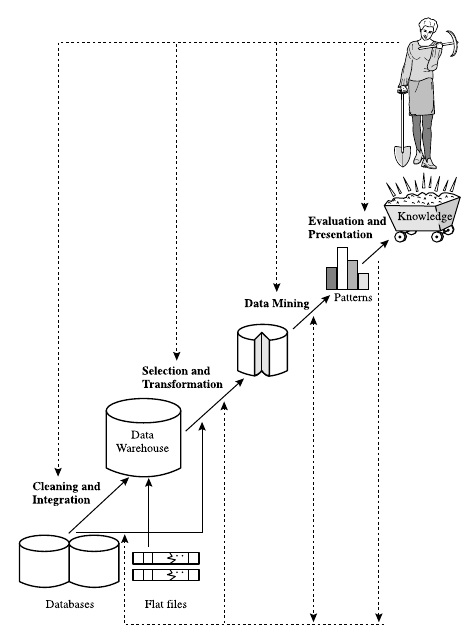
\includegraphics[scale=1]{Gambar/tahapdatamining.jpg}
\caption[Tahap \textsl{Data Mining}, Sumber Data Mining Concepts and Techniques]{Tahap \textsl{Data Mining}, Sumber Data Mining Concepts and Techniques} 
\end{figure}

Tahap pertama hingga keempat merupakan bagian dari \textsl{data preprocessing}, dimana data-data disiapkan untuk dilakukan penggalian data. Tahap \textsl{data mining} merupakan tahap dimana melakukan penggalian data. Tahap keenam merupakan tahap pencarian pola yang merepresentasikan \textsl{knowledge}. Sedangkan tahap terakhir merupakan visualisasi dan representasi dari \textsl{knowledge} yang sudah diperoleh dari tahap sebelumnya.


\subsection{\textsl{Data Cleaning}}
\textsl{Data cleaning} merupakan tahap \textsl{data mining} untuk menghilangkan \textsl{missing value} dan \textsl{noisy data}. Pada umumnya, \textsl{data} yang diperoleh dari \textsl{database} terdapat nilai yang tidak sempurna seperti nilai yang hilang, nilai yang tidak valid atau bahkan salah ketik. Nilai-nilai tersebut dapat diatasi dengan cara \textsl{smoothing techniques}. Atribut dari suatu \textsl{database} yang tidak relevan atau redudansi bisa diatasi dengan menghapus atribut tersebut. 

\subsubsection{\textsl{Missing Values}}
\textsl{Missing values} akan mengganggu proses \textsl{data mining} pada komputer dan dapat menghasilkan nilai akhir yang tidak sesuai. Terdapat beberapa teknik untuk mengatasi \textsl{missing values} yaitu
	\begin{itemize}
		\item Membuang tuple yang terdapat nilai yang hilang\textit{\textit{}}
		\item Mengisi nilai yang hilang secara manual
		\item Mengisi nilai yang hilang dengan menggunakan nilai konstan yang bersifat umum
		\item Menggunakan nilai rata-rata dari suatu atribut untuk mengisi nilai yang hilang
	\end{itemize}
\subsubsection{\textsl{Noisy Data}}
\textsl{Noisy data} merupakan nilai yang berasal dari error atau tidak valid. \textsl{Noisy data} dapat dihilangkan dengan menggunakan teknik \textsl{smoothing}. Terdapat 3 metode untuk menghilangkan \textsl{noisy data} yaitu
	\begin{itemize}
		\item \textsl{Binning}, merupakan metode pengisian data sesuai dengan proses yang dilakukan pada data tersebut
		\item \textsl{Regression}, merupakan metode yang mencari persamaan atribut untuk memprediksikan suatu nilai
		\item	\textsl{Clustering}, merupakan metode pengelompokan dimana ditemukan \textsl{outliers} yang dapat dibuang
	\end{itemize}

%\subsubsection{\textsl{Data Cleaning as a Process}}
%Tahap pertama pada \textsl{data cleaning} adalah \textsl{discrepancy detection}. Ketidakcocokan dapat dikarenakan oleh beberapa faktor, termasuk desain data yang buruk, kesalahan manusia ketika memasukan data, dan data yang sudah kadarluarsa. Ketidakcocokan ini juga dapat disebabkan tidak konsisten representasi data dan kode atau dikarenakan kesalahan perangkat ketika melakukan pemasukan data.

%Untuk mempermudah pencarian ketidakcocokan tersebut, kita dapat membuat sebuah data yang berisi informasi mengenai data atau biasa disebut \textsl{metadata}. Pada tahap ini, penulisan \textsl{script} bisa ditulis dengan cara masing-masing. Disini, dapat ditemukan \textsl{noise}, \textsl{outliers}, dan nilai-nilai yang tidak cocok atau tidak konsisten.

%Data juga harus diperiksa dengan \textsl{unique rules}, \textsl{consecutive rules}, dan \textsl{null rules}. \textsl{unique rules} mengatakan bahwa setiap nilai dari sebuah atribut harus berbeda dengan nilai yang lain pada atribut tersebut. \textsl{Consecutive rules} mengatakan bahwa tidak boleh ada nilai yang hilang diantara nilai tertinggi dan terendah untuk sebuah atribut, dan semua nilai harus bersifat unik. \textsl{null rules} menspesifikasikan penggunaan nilai \textsl{blanks} atau kosong, tanda tanya, karakter spesial, atau \textsl{string} yang dapat menandakan bahwa nilai tersebut bersifat kosong.

%Tahap deteksi ketidakcocokan ini dapat dibantu juga dengan menggunakan \textbf{data scrubbing tools} dan \textbf{data auditing tools}. \textbf{data scrubbing tools} akan menggunakan sebuah domain data untuk melakukan pencarian ketidakcocokan data dan membetulkan data tersebut dengan menggunakan teknik \textsl{parsing} dan \textsl{fuzzy matching}. \textbf{Data auditing tools} akan mencari ketidakcocokan dengan melakukan analisa data untuk menemukan \textsl{rules}, relasi, dan mendeteksi data yang melanggar hal tersebut.

%Beberapa data dapat diperbaiki dengan cara manual, namun sebagian besar data akan membutuhkan \textsl{data transformation} untuk membetulkan data tersebut.

\subsection{\textsl{Data Integration}}
\textsl{Data integration} merupakan tahap menggabungkan data dari berbagai sumber. Sumber tersebut bisa termasuk beberapa \textsl{database}, \textsl{data cubes}, atau bahkan \textsl{flat data}. \textsl{Data cube} merupakan teknik pengambilan data-data dari \textsl{data warehouse} dan dilakukan operasi agregasi sesuai dengan kondisi tertentu (contoh, penjumlahan total penjualan per tahun dari 2005-2010). Sedangkan \textsl{flat data} merupakan data yang disimpan dengan cara apapun untuk merepresentasikan database model pada sebuah data baik berbentuk \textsl{plain text file} maupun \textsl{binary file}. 

Tahap ini harus dilakukan secara teliti terutama ketika dalam memasangkan nilai-nilai yang berasal dari sumber yang berbeda. Pada tahap ini, perlu dilakukan identifikasi data apakah data tersebut dapat diturunkan atau tidak agar data yang diperoleh tidak terlalu besar. \textsl{Data integration} yang baik merupakan integrasi yang dapat memaksimalkan kecepatan dan meningkatkan akurasi dari proses \textsl{data mining}. Contoh studi kasus dari \textsl{data integration}, jika suatu perusahaan sepatu A memiliki dua pabrik dengan \textsl{database} lokal pada masing-masing pabrik, jika akan dilakukan \textsl{data mining} pada kedua \textsl{database }tersebut, maka kedua \textsl{database} akan digabung dan perlu diperhatikan serta diperbaiki nilai-nilai seperti \textsl{primary key}, atribut, dan lain-lain agar tidak terjadi \textsl{error} pada \textsl{database} yang sudah digabung. Proses dari penggabungan hingga perbaikan nilai-nilai pada kedua database tersebut adalah proses \textsl{data integration}.

\subsection{\textsl{Data Selection}}
Proses dimana data-data yang relevan dengan analisis akan diambil dari database dan data yang tidak relevan akan dibuang. Sebagai contoh kasus, jika akan dilakukan analisa mengenai nilai mahasiswa dalam satu semester, atribut pada tabel nilai sebagai berikut
	\begin{itemize}
		\item NPMMahasiswa
		\item NamaMahasiswa
		\item JenisKelamin
		\item Alamat
		\item MataKuliah
		\item NilaiART
		\item NilaiUTS
		\item NilaiUAS
	\end{itemize}
Maka, atribut yang akan diambil adalah MataKuliah, NilaiART, NilaiUTS, NilaiUAS, sedangkan atribut yang akan dibuang adalah NPMMahasiswa, NamaMahasiswa JenisKelamin, dan Alamat karena tidak terlalu berhubungan dengan analisa.

\subsection{\textsl{Data Transformation}}
\textsl{Data transformation} merupakan tahap pengubahan data agar siap dilakukan proses \textsl{data mining}. \textsl{Data transformation} bisa melibatkan,
	\begin{itemize}
		\item \textsl{Smoothing}, proses untuk membuang \textsl{noise} seperti yang dilakukan pada tahap \textsl{data cleaning}
		\item \textsl{Aggregation}, proses mengganti nilai-nilai menjadi suatu nilai yang dapat mewakili nilai sebelumnya
		\item \textsl{Generalization}, proses dimana membuat suatu nilai yang bersifat khusus menjadi nilai yang bersifat umum
		\item \textsl{Normalization}, proses dimana suatu nilai dapat diubah skalanya menjadi nilai yang lebih kecil dan spesifik
		\item \textsl{Attribute construction}, proses membuat atribut baru yang berasal dari beberapa atribut untuk membantu proses data mining
	\end{itemize}
	
\subsubsection{\textsl{Normalization}}
Atribut dapat dinormalisasi dengan memberi skala pada nilainya sehingga nilai tersebut menjadi suatu range yang lebih spesifik dan kecil seperti 0,0 sampai 1,0.
Dua teknik nnormalisasi yaitu, \textsl{min-max normalization} dan \textsl{z-score normalization}. \textsl{Min-max normalization} akan mengubah semua nilai menjadi nilai dengan skala tertentu. Dengan menggunakan rumus 

\begin{displaymath}
	\nu' = \frac{\nu-min_{A}}{max_{A}-min_{A}}(newMax_{A}-newMin_{A})+newMin_{A}	
\end{displaymath}

Contoh kasus, misalkan nilai minimun dan maximum dari suatu pendapatan adalah 12.000 dan 98.000, akan diubah menjadi berskala antara 0,0 sampai 1,0. Jika ada nilai pendapat yang baru, yaitu 73.600, maka akan menjadi

\begin{displaymath}
\frac{73.600-12.000}{98.000-12.000} (1,0-0)+0 = 0,716
\end{displaymath}

\textsl{z-score normalization} merupakan normalisasi berdasarkan nilai rata-rata dan standar deviasi dari nilai-nilai atribut dengan cara

\begin{displaymath}
\nu' = \frac{\nu-\overline{A}}{\sigma_{A}}
\end{displaymath}

Contoh kasus, misal nilai rata-rata dan standar deviasi dari nilai-nilai atribut pendapatan adalah 54.000 dan 16.000. Dengan \textsl{z-score}, jika ada nilai pendapatan baru yaitu 73600, maka akan diubah menjadi

\begin{displaymath}
\frac{73.600-54.000}{16.000} = 1,225 
\end{displaymath}

\subsubsection{\textsl{Attribute Construction}}
\textsl{Attribute Construction} merupakan teknik menambahkan atribut baru yang berdasarkan dari atribut yang sudah ada guna menambah akurasi. Contoh kasus, dibuat atribut baru bernama area berdasarkan atribut panjang dan lebar. 

\subsubsection{\textsl{Data Reduction}}
Proses \textsl{aggregation} dan \textsl{generalization} akan dilakukan dalam bentuk proses \textsl{data reduction} dan \textsl{Data Cube Aggregation}.
\textsl{Data reduction} dan dilakukan untuk mendapatkan nilai yang representif namun tetap menjaga keakuratan hasil \textsl{data mining}. Terdapat beberapa cara dalam mengimplementasikan \textsl{data reduction} yaitu
	\begin{itemize}
		\item \textsl{Data subset selection}
		\item \textsl{Dimensionality reduction}
		\item \textsl{Numerosity reduction}
		\item \textsl{Discretization and concept hierarchy generation}
	\end{itemize}	

\subsubsection {\textsl{Attribute Subset Selection}}
\textsl{Attribute subset selection} merupakan salah satu cara melakukan \textsl{data reduction} dengan menghilangkan atribut-atribut yang tidak relevan atau data yang redudansi. Hal ini dapat mempermudah pencarian pola dikarenakan banyak atribut yang muncul akan berkurangnya. 

\subsubsection {\textsl{Dimensionality Reduction}}
\textsl{Dimensionality Reduction} merupakan metode pengurangan nilai secara acak dengan cara melakukan konversi data. Jika data original dapat dibuat ulang dari data yang sudah dikompresi tanpa kehilangan informasi, maka akan dikatakan \textsl{lossless}, namun jika hanya mendapatkan data pendekatannya saja, akan disebut lossly [1].

\subsubsection {\textsl{Numerosity Reduction}}
\textsl{Numerosity Reduction} merupakan metode dimana data diganti atau ditentukan dengan cara parametik atau nonparametrik.

\subsubsection {\textsl{Discretization and Concept Hierarchy Generation}}
lewat dulu

\subsection{\textsl{Data Mining}}

\subsubsection{\textsl{Classification and Prediction}}
\textsl{Classification} merupakan pemodelan yang dibangun untuk memprediksikan label kategori, seperti "`baik"', "`cukup"', dan "`buruk"' dalam sistem penilaian sikap seorang siswa atau "`mini bus"', "`bus"', atau "`sedan"' dalam kategori tipe mobil. Kategori tersebut dapat direpresentasikan dengan menggunakan nilai \textsl{discrete}. Nilai \textsl{discrete} merupakan nilai yang terpisah dan berbeda, seperti 1 atau 5. Kategori yang direpresentasikan oleh nilai \textsl{discrete} maka akan menjadi nilai yang terurut dan tidak memiliki arti, seperti 1,2,3 untuk merepresentasikan kategori tipe mobil "`mini bus"', "`bus"', dan "`sedan"'.

\textsl{Prediction} merupakan model yang dibangun untuk meramalkan \textsl{continuous-value function} atau \textsl{ordered value}. \textsl{Ordered value} merupakan nilai yang terurut dan berlanjut. contoh studi kasus untuk pemodelan prediction adalah seorang marketing ingin meramalkan seberapa banyak konsumen yang akan belanja di sebuah toko dalam waktu satu bulan. Pemodelan tersebut disebut \textsl{predictor}.\textsl{Regression Analysis}, merupakan metodologi statistik yang digunakan untuk \textsl{numeric prediction}. \textsl{Classification} dan \textsl{numeric prediction} merupakan dua jenis utama dalam masalah prediksi.

\textsl{Data Classification} merupakan proses untuk melakukan klasifikasi. \textsl{Data classification} memiliki dua tahap proses, yaitu \textsl{learning step} dan tahap klasifikasi seperti pada ilustrasi di gambar 2.2. \textsl{Learning step} merupakan langkah pembelajaran, di mana algoritma klasifikasi membangun \textsl{classification rules} (yang berisi syarat atau aturan sebuah nilai masuk ke dalam kategori tertentu) dengan cara menganalisis \textsl{training set} yang merupakan \textsl{database tuple}. Karena pembuatan \textsl{classification rules} menggunakan \textsl{training set}, yang dikenal juga sebagai \textsl{supervised learning}. 
Pada tahap kedua, dilakukan proses klasifikasi nilai berdasarkan \textsl{classification rules} yang sudah dibangun dari tahap pertama.

\begin{figure}
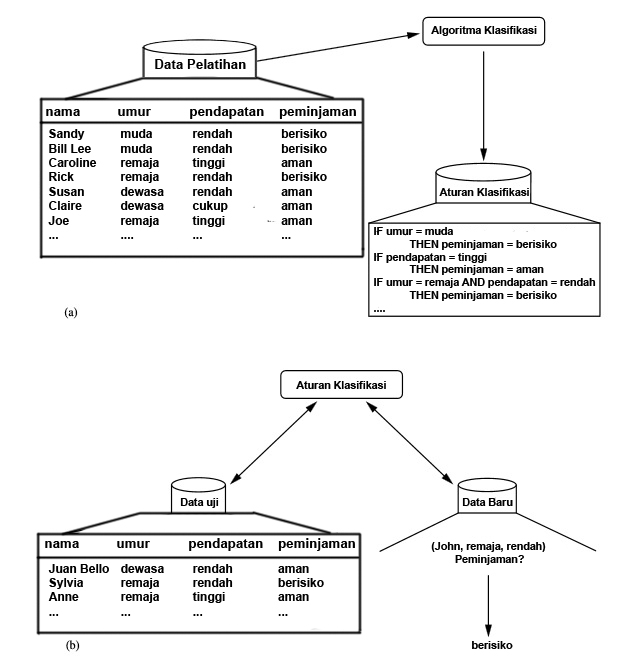
\includegraphics[scale=1]{Gambar/tahapdataclassification.jpg}
\caption[Tahap \textsl{Data Mining}, Sumber Data Mining Concepts and Techniques]{proses \textsl{data classification}, Sumber Data Mining Concepts and Techniques} 
\end{figure}

\subsection{\textsl{Decision Tree}}
Salah satu cara pembuatan \textsl{classification rules} pada \textsl{Data Classification} adalah dengan membuat \textsl{decision tree} (pohon keputusan). \textsl{Decision tree} merupakan \textsl{flowchart} yang berbentuk pohon, dimana setiap node internal (\textsl{nonleaf} node) merupakan hasil test dari atribut, setiap cabang merepresentasikan output dari test, dan setiap node daun memiliki \textsl{class label}. Bagian paling atas dari pohon disebut \textsl{root node}. Contoh studi kasus, pohon keputusan untuk menentukan apakah seorang konsumen akan membeli komputer atau tidak (ilustrasi pohon keputusan pada gambar 2.3) 

\begin{figure}
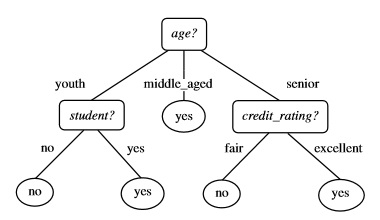
\includegraphics[scale=1]{Gambar/decisiontree.jpg}
\caption[Tahap \textsl{Data Mining}, Sumber Data Mining Concepts and Techniques]{proses \textsl{data classification}, Sumber Data Mining Concepts and Techniques} 
\end{figure}

subsubsection{\textsl{Decision Tree Induction}}
\textsl{Decision tree induction} merupakan pelatihan pohon keputusan dari tupel pelatihan kelas berlabel. Terdapat tiga teknik untuk membuat \textsl{decission tree} yaitu ID3, C4.5 dan Classification and Regression Trees (CART). ketiga teknik tersebut menggunakan pendekatan \textsl{greedy} yang merupakan \textsl{decission tree} yang dibangun secara \textsl{top-down recursive divide and conquer}. Berikut algoritma untuk membuat pohon keputusan dari suatu tupel pelatihan.

Input:
\begin{itemize}
	\item Partisi data, D, merupakan set data pelatihan dan kelas label
	\item \textsl{attribute\_list}, merupakan set dari atribut kandidat
	\item \textsl{Attribute\_selection\_method}, prosedur untuk menentukan \textsl{splitting criterion}. Pada input ini, terdapat juga data \textsl{splitting\_attribute} dan mungkin salah satu dari \textsl{split point} atau \textsl{splitting subset}
\end{itemize}

Output: pohon keputusan

Method:

(1) create a node N;

(2) if tuples in D are all of the same class, C then

(3)	return N as a leaf node labeled with the class C;

(4)	if attribute\_list is empty then

(5) return N as leaf node labeled with the majority class in D; //majority voting

(6)	apply Attribute\_selection\_method(D, atribute\_list) to find the "`best"' splitting\_criterion;

(7) label node N with splitting\_criterion;

(8) if splitting\_attribute is discrete valued and
				multiway splits allowed then //not restricted to binary trees

(9) attribute\_list <- attribute\_list - splitting\_attribute; //remove splitting\_attribute

(10)for each outcome j of splitting\_criterion // partition the tuples and from subtrees for each partition

(11)let D\lowercase{j} be the set of data tuples in D satisfying outcome j; //a partition

(12) if D\lowercase{j} is empty then

(13) attach a leaf labeled with the majority class in D to node N;

(14) else attach the node returned by generate\_decision\_tree(D\lowercase{j}, attribute\_list) to node N;

endfor

(15) return N;


Pohon keputusan akan dimulai dengan satu node, yaitu N, merepresentasikan tuple pelatihan pada D (langkah 1)

Jika tuple di D memiliki kelas yang sama semua, maka node N akan menjadi daun dan diberi label dari kelas tersebut (langkah 2 dan 3). Perlu diketahui bahwa langkah 4 dan 5 akan mengakhiri kondisi.

Jika tuple di D ada kelas yang berbeda, maka algoritma akan memanggil \textsl{attribute\_selection\_method} untuk menentukan \textsl{splitting criterion}. \textsl{Splitting criterion} akan menentukan atribut pada node N yang merupakan nilai terbaik untuk memecah nilai atribut pada tuple ke dalam kelas masing-masing. (langkah 6)

Node N akan diisi dengan hasil dari \textsl{splitting criterion} (langkah 7). Kemudian kriteria tersebut agak dibentuk cabangnya masing-masing sesuai pada langkah 10 dan 11. Terdapat tiga kemungkinan bentuk kriteria jika A merupakan \textsl{splitting\_attribute} yang memiliki nilai unik seperti \{a1, a2, ..., av\}, yaitu,

\begin{enumerate}
	\item \textsl{Discrete valued}: cabang yang dihasilkan memiliki kelas dengan nilai diskret. Karena kelas yang dihasilkan diskret dan hanya memiliki nilai yang sama pada cabang tersebut, maka \textsl{attribut\_list} akan dihapus (langkah 8 dan 9)
	\item \textsl{Continuous values}: cabang yang dihasilkan memiliki jarak nilai untuk memenuhi suatu kondisi (contoh: A <= split\_point), dimana nilai \textsl{split\_point} adalah nilai pembagi yang dikembalikan oleh \textsl{attribute\_selection\_method}
	\item \textsl{Dicrete valued and a binary tree}: cabang yang dihasilkan adalah dua berupa nilai iya atau tidak dari "`apakah A anggota Sa"', dimana Sa merupakan subset dari A, yang dikembalikan oleh \textsl{Attribute\_selection\_method}
\end{enumerate}

Kemudian, akan dipanggil kembali algoritma \textsl{decision tree} untuk setiap nilai hasil pembagian pada tuple, Dj  (langkah 14).

Rekursif tersebut akan berhenti ketika salah satu dari kondisi terpenuhi, yaitu

\begin{enumerate}
	\item Semua tuple pada partisi D merupakan bagian dari kelas yang sama.
	\item Sudah tidak ada atribut yang dapat dilakukan pembagian lagi (dilakukan pengecekan pada langkah 4). Disini, akan dilakukan \textsl{majority voting} (langkah 5) yang akan mengkonversi node N menjadi \textsl{leaf} dan diberi label dengan kelas yang terbanyak pada D.
	\item Sudah tidak ada tuple yang dapat diberi cabang, Dj sudah kosong (langkah 12) dan \textsl{leaf} akan dibuat dengan \textsl{majority class} pada D (langkah 13).
\end{enumerate}

Pada langkah 15, akan dikembalikan nilai \textsl{decision tree} yang telah dibuat.

subsubsection{\textsl{Attribute Selection Measure}}

\textsl{Attribute Selection Measure} merupakan suatu hirarki untuk pemilihan \textsl{splitting criterion} yang terbaik yang memisah partisi data (D), tuple pelatihan kelas label ke dalam kelas masing-masing. \textsl{Attribute Selection Measure} menyediakan peringkat untuk setiap atribut pada training tuple. Jika \textsl{splitting criterion} merupakan nilai \textsl{continous} atau \textsl{binary trees}, maka nilai \textsl{split point} dan \textsl{splitting subset} harus ditentukan sebagai bagian dari \textsl{splitting criterion}. Contoh dari \textsl{attribute selection measure} adalah \textsl{information gain}, \textsl{gain ratio}, dan \textsl{gini index}.

Notasi yang digunakan adalah sebagai berikut. D merupakan data partisi, set pelatihan dari \textsl{class-labeled} tuple. Jika label kelas atribut memiliki m nilai yang berbeda yang mendifinisikan m kelas yang berbeda, Ci (for i=1,...,m). Ci,d menjadi kelas tuple dari Ci di D. |D| dan |Ci,d| merupakan banyak tuple pada D dan Ci,d.

\subsubsection{\textsl{Information Gain}}
ID3 menggunakan \textsl{information gain} sebagai \textsl{attribute selection measure} yang melakukan pemilihan atribut berdasarkan informasi yang terkandung dalam pesan. 


\subsection{\textsl{Pattern Evaluation}}
\textsl{Pattern evaluation} merupakan tahap mengidentifikasi apakah \textsl{pattern} atau pola tersebut menarik dan merepresentasikan \textsl{knowledge} berdasarkan beberapa \textsl{interestingness measures}.
Suatu \textsl{pattern} atau pola dapat dinyatakan menarik apabila
\begin{itemize}
	\item mudah dimengerti oleh manusia
	\item valid untuk data percobaan maupun data yang baru
	\item memiliki potensi atau berguna
	\item merepresentasikan \textsl{knowledge}
\end{itemize}

\subsection{\textsl{Knowledge Presentation}}
\textsl{Knowledge presentation} merupakan tahap representasi dan visualisasi terhadap \textsl{knowledge} yang merupakan hasil dari \textsl{knowledge discovery}.	
%\section{\textsl{Spatial and Spatiotemporal}}

\section{Log Histori KIRI}

KIRI memiliki log histori yang melakukan pencatatan untuk setiap user ketika menggunakan KIRI. \textsl{Log} tersebut memiliki 5 \textsl{field} untuk setiap \textsl{entry} sebagai berikut:
\begin{itemize}
	\item logId, primary key dari entry
	\item APIKey, mengidentifikasikan sumber dari pencarian ini
	\item \textsl{Timestamp} (UTC), waktu ketika pengguna KIRI mencari rute angkot menggunakan waktu UTC / GMT
	\item \textsl{Action}, tipe log, untuk penelitian ini selalu berisi FINDROUTE
	\item AdditionalData, mencatat koordinat awal, koordinat akhir, dan banyak rute yang ditemukan pada pencarian ini
\end{itemize}

LogId merupakan \textsl{field} dengan tipe data int dengan batas 6 karakter yang digunakan sebagai \textsl{primary key} dari tabel tersebut. LogId diisi dengan menggunakan fungsi \textsl{increment integer}. \textsl{Increment integer} merupakan fungsi untuk pengisian data pada database dengan menambahkan nilai 1 dari nilai yang terakhir kali diisi.
APIKey merupakan \textsl{field} dengan tipe data varchar yang digunakan untuk memeriksa pengguna KIRI ketika menggunakan KIRI.
\textsl{Timestamp} (UTC) merupakan \textsl{field} dengan tipe data \textsl{timestamp} yang digunakan untuk mencatat waktu penggunaan KIRI oleh user, diisi dengan menggunakan fungsi \textsl{current time}. \textsl{Current time} merupakan fungsi untuk pengisian data pada database dengan mengambil waktu pada komputer ketika record dibuat.
\textsl{Action} merupakan \textsl{field} dengan tipe data varchar yang digunakan untuk memeriksa fungsi apa yang dipanggil dari API KIRI. Terdapat beberapa tipe pada \textsl{field} ini, yaitu
/\begin{itemize}
	\item \textsl{ADDAPIKEY}, \textsl{action} yang dicatat ke dalam log ketika fungsi pembuatan \textsl{API key} yang baru dipanggil.
	\item \textsl{FINDROUTE}, \textsl{action} yang dicatat ketika user melakukan pencarian rute
	\item \textsl{LOGIN}, \textsl{action} yang dicatat ketika developers melakukan login dengan menggunakan \textsl{API key}
	\item \textsl{NEARBYTRANSPORT}, \textsl{action} yang dicatat ketika user mencari transportasi di daerah rute sedang dicari
	\item \textsl{PAGELOAD}, \textsl{action} yang dicatat ketika user memasuki halaman KIRI
 	\item \textsl{REGISTER},\textsl{action} yang dicatat ketika developers melakukan pendaftaran pada KIRI \textsl{API key}
	\item \textsl{SEARCHPLACE}, \textsl{action} yang dicatat ketika user memanggil fungsi pencarian lokasi dengan menggunakan nama tempat
	\item \textsl{WIDGETERROR}, mencatat log tersebut ketika user menerima error dari \textit{widget}
	\item \textsl{WIDGETLOAD}, mencatat log tersebut ketika user mengdownload widget
\end{itemize}
AdditionalData, merupakan \textsl{field} dengan tipe data varchar yang digunakan untuk mencatat informasi yang dibutuhkan sesuai dengan \textsl{field action}.}{}
\ifdefstring{\vbabc}{1}{\chapter{Analisa}

Pada bab ini, akan dilakukan analisa terhadap data yang akan diproses menggunakan \textsl{data mining} dan perangkat lunak yang akan dibangun untuk melakukan proses data tersebut.

\section{Analisis Data}
\label{analisisData}
Pada bab ini, akan dilakukan analisa \textsl{preprocessing data} yang meliputi \textsl{data cleaning}, \textsl{data integration}, \textsl{data selection} dan \textsl{data transformation}. Setelah membaca dan menganalisis data \textsl{log} histori KIRI, maka penelitian ini akan lebih fokus untuk meneliti mengenai lokasi keberangkatan dan tujuan dari user yang menggunakan aplikasi KIRI.

\subsection{Data Cleaning}
Pada tahap ini, data yang akan menjadi input akan diperiksa apakah mengandung \textsl{missing value} atau \textsl{noisy}. Setelah dilakukan pemeriksaan, tidak ditemukan \textsl{missing value} ataupun \textsl{noisy}, sehingga tahap ini dapat dilewat.

\subsection{Data Integration}
Pada tahap ini, data-data dari beberapa database akan digabung dan diintegrasikan menjadi satu database. Karena data yang digunakan hanya berasal dari satu tabel, maka tahap ini dapat dilewat.

\subsection{\textsl{Data Selection}}
Pada tahap ini, akan dilakukan pemilihan data yang akan digunakan. Pada penelitian ini, akan dilakukan proses \textsl{data mining} mengenai lokasi keberangkatan dan tujuan dari seorang user yang menggunakan aplikasi KIRI. Oleh karena itu, pada atribut \textsl{action}, nilai yang akan dipilih hanya \textsl{FINDROUTE}. Hal ini dikarenakan, hanya \textsl{action FINDROUTE} yang menjelaskan posisi keberangkatan dan tujuan dari user. Selain itu, data tersebut terlihat menarik karena dimungkinkan dapat menghasilkan suatu pola yang membantu melakukan klasifikasi mengenai perpindahan penduduk khususnya untuk daerah Bandung. Karena seluruh \textsl{action} bernilai satu jenis yaitu \textsl{FINDROUTE}, maka atribut tersebut dapat dihilangkan. Selain itu, atribut logId dan APIKey tidak akan dimasukan ke dalam proses karena tidak memiliki hubungan dengan lokasi keberangkatan dan tujuan dari seorang user.

Dari analisis diatas, maka atribut yang dipilih untuk diproses ke dalam \textsl{data mining} adalah
\begin{itemize}
	\item \textsl{Timestamp} (UTC)
	\item \textsl{AdditionalData}
\end{itemize}

Berikut contoh data dari atribut tersebut dapat dilihat pada tabel \ref{table:contohDataLog}
\begin{table}[h]
\caption{Contoh data \textsl{log} KIRI setelah \textsl{data selection}}
\label{table:contohDataLog}
\begin{tabular}{|l|l|}
\hline
\textbf{Timestamp (UTC)} & \textbf{AdditionalData}                     \\ \hline
2/1/2014 0:11            & -6.8972513,107.6385574/-6.91358,107.62718/1 \\ \hline
2/1/2014 0:13            & -6.8972513,107.6385574/-6.91358,107.62718/1 \\ \hline
2/1/2014 0:16            & -6.90598,107.59714/-6.90855,107.61082/1     \\ \hline
2/1/2014 0:18            & -6.9015366,107.5414474/-6.88574,107.53816/1 \\ \hline
2/1/2014 0:25            & -6.90608,107.61530/-6.89140,107.61060/2     \\ \hline
2/1/2014 0:27            & -6.89459,107.58818/-6.89876,107.60886/2     \\ \hline
2/1/2014 0:28            & -6.89459,107.58818/-6.86031,107.61287/2     \\ \hline
\end{tabular}
\end{table}

Pada atribut \textsl{additionalData}, jika nilai atribut \textsl{action} adalah \textsl{FINDROUTE}, maka nilai \textsl{additionalData} memiliki tiga bagian yang dibatasi dengan '/'. Ketiga bagian tersebut adalah

\begin{enumerate}
	\item Nilai latitude dan longitude dari lokasi keberangkatan yang dipilih oleh user
	\item Nilai latitude dan longitude dari lokasi tujuan yang dipilih oleh user
	\item Nilai yang menunjukkan banyak jalur yang dihasilkan oleh sistem KIRI
\end{enumerate}

Nilai dari banyak jalur akan dibuang ketika memasuki tahap \textsl{data transformation}, karena nilai tersebut hanya menunjukkan banyak jalur tetapi user pasti hanya memilih salah satu dari jalur tersebut, sehingga nilai jalur ini dapat diasumsikan memiliki nilai 1 semua. karena kolom jalur bernilai satu semua, maka kolom tersebut dapat dibuang.

\subsection{\textsl{Data Transformation}}
Pada tahap ini, akan dilakukan perubahan data. Pada atribut yang dipilih, nilai dari atribut \textsl{timestamp} dan \textsl{additionaldata} perlu dilakukan transformasi agar program dapat membaca dan memproses data lebih cepat. 

Pada atribut \textsl{timestamp}, nilai waktu dari atribut tersebut akan diubah menjadi waktu GMT+8. Kemudian, data akan diubah menjadi empat atribut, yaitu:
\begin{itemize}
	\item Bulan, atribut ini akan menunjukkan bulan ketika user KIRI memanggil \textsl{action FINDROUTE}, dengan nilai antara 01 sampai 12. Nilai tersebut dapat diperoleh dengan cara mengambil nilai string dari timpestamp yang berada di antara garis miring pertama dan kedua.
	\item Tahun, atribut ini akan menunjukkan tahun ketika user KIRI memanggil \textsl{action FINDROUTE}, dengan format empat angka (contoh: 2014). Nilai tersebut dapat diperoleh dengan cara mengambil nilai string dari timpestamp yang berada di antara garis miring kedua dan spasi.
	\item Hari, atribut ini akan menunjukkan hari ketika user KIRI memanggil \textsl{action FINDROUTE}, dengan range nilai antara senin sampai minggu. Nilai tersebut dapat diperoleh dengan cara melakukan memanggil \textsl{method} pencarian hari berdasarkan tanggal dari timestamp pada java.
	\item Jam, atribut ini akan menunjukkan jam ketika user KIRI memanggil \textsl{action FINDROUTE}, dengan range nilai antara 00 sampai 23. Nilai tersebut dapat diperoleh dengan cara mengambil nilai string dari timpestamp yang berada di antara spasi dan titik dua.
\end{itemize}

Data \textsl{timestamp} diubah menjadi enam bagian, agar dapat dilakukan pengelompokan yang dilihat dari tanggal, bulan, tahun, hari, jam dan menit.

Pada atribut \textsl{additionalData}, data akan diubah menjadi empat atribut, yaitu:
\begin{itemize}
	\item Latitude keberangkatan, atribut ini berisi nilai latitude dari lokasi keberangkatan yang dipilih oleh user. Nilai tersebut dapat diperoleh dengan cara mengambil nilai string sebelum koma yang pertama.
	\item Longitude keberangkatan, atribut ini berisi nilai longitude dari lokasi keberangkatan yang dipilih oleh user. Nilai tersebut dapat diperoleh dengan cara mengambil nilai string yang berada di antara koma pertama dan garis miring pertama.
	\item Latitude tujuan, atribut ini berisi nilai latitude dari lokasi tujuan yang dipilih oleh user. Nilai tersebut dapat diperoleh dengan cara mengambil nilai string di antara garis miring yang pertama dan koma kedua.
	\item Longitude tujuan, atribut ini berisi nilai longitude dari lokasi tujuan yang dipilih oleh user. Nilai tersebut dapat diperoleh dengan cara mengambil nilai string yang berada di antara koma kedua dan garis miring kedua.
\end{itemize}

Data \textsl{additionalData} diubah menjadi empat bagian, agar program dapat membaca data tersebut lebih mudah.

Dari analisis diatas, banyak atribut dari tabel \textsl{statistics} akan menjadi delapan, yaitu:
\begin{itemize}
	\item Bulan
	\item Tahun
	\item Hari
	\item Jam
	\item Latitude Keberangkatan
	\item Longitude Keberangkatan
	\item Latitude Tujuan
	\item Longitude Tujuan
\end{itemize}

Contoh hasil data transformasi jika input merupakan data dari tabel \ref{table:contohDataLog} dapat dilihat pada tabel \ref{table:contohHasilDataTransformasi}	.

\begin{center}
\begin{table}
\rotatebox{90}{%
%\begin{tabular}{|@{}>{\raggedright}p{.2\textheight}>{\raggedright}p{.2\textheight}>{\raggedright}p{.2\textheight}>{\raggedright\arraybackslash}p{.2\textheight}@{}|
\begin{tabular}{|l|l|l|l|p{2.5cm}|p{2.5cm}|p{2.5cm}|p{2.5cm}|}
\hline
\textbf{Bulan}	& \textbf{Tahun} 	& \textbf{Hari} & \textbf{Jam} & \textbf{Latitude Keberangkatan} & \textbf{Longitude Keberangkatan} & \textbf{Latitude Tujuan} & \textbf{Longitude Tujuan}      \\ \hline
02								& 2014						& Sabtu         & 00						 & -6.8972513										 & 107.6185574 							  & -6.91358                & 107.62718 \\ \hline
02								& 2014						& Sabtu         & 00						 & -6.8972513										 & 107.6385574                & -6.91358							  & 107.62718 \\ \hline
02								& 2014						& Sabtu         & 00 						 & -6.90598											 & 107.59714     		  				& -6.90855						&107.61082 \\ \hline
02								& 2014						& Sabtu         & 00  					 & -6.9015366										 & 107.5414474 								& -6.88574					    & 107.53816 \\ \hline
02								& 2014						& Sabtu         & 00 						 & -6.90608										   & 107.61530     						  & -6.89140					 &107.61060 \\ \hline
02								& 2014						& Sabtu         & 00 						 & -6.89459											 & 107.58818     							& -6.89876						&107.60886 \\ \hline
02								& 2014						& Sabtu         & 00 						 & -6.89459											 &107.58818  								   & -6.86031					 &107.61287 \\ \hline
\end{tabular}%
}
\caption{Contoh hasil data transformasi}
\label{table:contohHasilDataTransformasi}
\end{table}
\end{center}

Agar dapat diperoleh \textsl{decision tree} mengenai lokasi keberangkatan dan tujuan dari user KIRI, maka atribut kelas yang akan digunakan adalah nilai latitude dan longitude dari lokasi keberangkatan dan tujuan. Karena atribut kelas ada empat, maka akan dilakukan penyederhanaan dari keempat atribut untuk meningkatkan akurasi serta tingkat efisien proses \textsl{data mining}. 

Nilai \textsl{latitude} serta \textsl{longitude} dari data lokasi keberangkatan dan tujuan akan diubah menjadi nilai yang menunjukkan apakah daerah lokasi keberangkatan dan tujuan tersebut menunjukkan perjalanan keluar dari Bandung atau tidak. Hal ini dilakukan agar diperoleh data perbandingan pergerakan penduduk, apakah mereka lebih banyak yang keluar dari Bandung atau sebaliknya berdasarkan waktu tertentu. Untuk menentukan hal tersebut, maka akan dibutuhkan klasifikasi daerah agar mudah dilakukan penentuan apakan \textsl{user} akan berangkat ke Bandung atau tidak. \textsl{Classification} daerah yang ditentukan setelah melihat peta Bandung dapat dilihat pada gambar \ref{fig:classificationMap}.

\begin{figure}
\centering
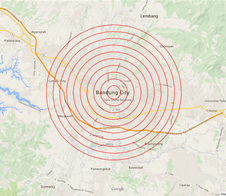
\includegraphics[scale=1]{Gambar/classificationmap.jpg}
\caption[\textsl{Classification} pada daerah Bandung]{\textsl{Classification} pada daerah Bandung}
\label{fig:classificationMap} 
\end{figure}

Penentuan \textsl{classification} tersebut berdasarkan perkiraaan titik pusat yang sudah ditentukan, yaitu -6.92036,107.60500 dalam latitude dan longitude. Kemudian dibagi menjadi sepuluh daerah yang memiliki perbedaan radius sebesar 1 km, sehingga diameter untuk daerah pertama adalah 2 km, diameter untuk daerah kedua adalah 4 km, dan seterusnya, untuk daerah terakhir (yaitu daerah 10) akan memiliki diameter 20 km.

Suatu lokasi atau titik latitude longitude dapat diketahui berada pada daerah yang mana dengan cara menghitung jarak titik tersebut dengan titik pusat yang sudah ditentukan (yaitu -6.92036,107.60500) dengan menggunakan rumus Haversine. Jika jarak yang diperoleh lebih kecil sama dengan 1 km, maka berada di daerah pertama, sedangkan jika jarak yang diperoleh lebih kecil sama dengan 2 km dan lebih besar dari 1 km, maka berada di daerah kedua, dan seterusnya, dan untuk daerah terakhir (yaitu daerah 10) titik akan memiliki jarak lebih kecil sama dengan 10 km dan lebih besar dari 9 km dengan titik pusat. Jika suatu titik memiliki jarak terhadap titik pusat lebih dari 10 km, maka akan menjadi daerah luar Bandung.

Setelah lokasi keberangkatan dan lokasi tujuan ditentukan daerahnya, dapat ditentukan apakah user tersebut menuju pusat Bandung atau tidak. Jika daerah dari lokasi keberangkatan lebih besar daripada daerah lokasi tujuan, maka user tersebut menuju pusat Bandung. Kemudian, jika daerah dari lokasi keberangkatan lebih kecil daripada daerah lokasi tujuan, maka user tersebut tidak menuju pusat Bandung. Sedangkan, jika lokasi keberangkatan dan lokasi tujuan berada di daerah yang sama, maka user tersebut maka user tersebut bergerak di daerah yang sama.

Dengan adanya perhitungan jarak dan penentuan daerah Bandung, nilai latitude dan longitude dari lokasi keberangkatan dan tujuan dapat dibuang dan diganti oleh atribut menujuBandung dengan tipe data \textsl{integer}. Jika isi dari atribut tersebut bernilai 1, maka \textsl{user} tersebut menuju Bandung sedangkan nilai 0 bearti \textsl{user} tidak menuju Bandung, dan jika nilai atribut tersebut adalah 2, maka \textsl{user} tersebut memiliki lokasi keberangkatan dan tujuan pada daerah yang sama. Contoh hasil data setelah dilakukan \textsl{transformation} terhadap latitude dan longitude terdapat pada tabel \ref{table:contohHasilDataTransformasiLatLong}.

\begin{table}[H]
\caption{Contoh hasil data transformasi latitude longitude}
\label{table:contohHasilDataTransformasiLatLong}
\begin{longtable}{|l|l|l|l|l|}
\hline
\textbf{Bulan}	& \textbf{Tahun} 	& \textbf{Hari} & \textbf{Jam}	& \textbf{MenujuBandung} \\ \hline
02								& 2014						& Sabtu         & 00         	& 2                    \\ \hline
02								& 2014						& Sabtu         & 00         	& 1        					  \\ \hline
02								& 2014						& Sabtu         & 00         	& 1       							\\ \hline
02								& 2014						& Sabtu         & 00         	& 0         						\\ \hline
02								& 2014						& Sabtu         & 00         	& 1          					\\ \hline
02								& 2014						& Sabtu         & 00         	& 2      							\\ \hline
02								& 2014						& Sabtu         & 00         	& 0       							\\ \hline
\end{longtable}
\end{table} 


\section{Analisis Perangkat Lunak}
Agar analisis pola dari lokasi keberangkatan dan tujuan dari data \textsl{log} histori lebih mudah, maka akan dibangun sebuah perangkat lunak yang dapat melakukan proses \textsl{data mining} dengan menggunakan teknik ID3 dan C4.5, serta dapat melakukan visualisasi hasil dari \textsl{data mining} yang diperoleh setelah proses dijalankan yaitu perangkat lunak \textsl{data mining log} histori KIRI. 

Perangkat lunak yang dibangun akan berbasis desktop dan menggunakan bahasa pemograman java. Pada subbab ini akan dibahas spesifikasi kebutuhan funsional, pemodelan perangkat lunak, diagram \textsl{use case}, skenario, diagram kelas dari Perangkat Lunak yang akan dibangun.

\subsubsection{Spesifikasi Kebutuhan Fungsional Perangkat Lunak \textsl{Data Mining log} Histori KIRI}
Spesifikasi kebutuhan perangkat lunak yang akan dibangun untuk melakukan \textsl{data mining log} histori KIRI yang sesuai yang diharapkan adalah
\begin{enumerate}
	\item Dapat menerima dan membaca input text yang sudah disiapkan
	\item Dapat melakukan \textsl{preprocessing} data sesuai dengan yang dijelaskan pada bab analisis data
	\item Dapat melakukan proses \textsl{data mining}, ID3 dan C4.5
	\item Dapat melakukan visualisasi hasil dari \textsl{data mining} yang diperoleh
\end{enumerate}

\subsubsection{Pemodelan Perangkat Lunak \textsl{Data Mining Log} Histori KIRI}
Perangkat lunak \textsl{data mining log} histori KIRI akan mendapat input data text dengan format .txt. Setelah program mendapatkan input dan user menekan tombol proses, maka data tersebut akan diubah terlebih dahulu sesuai pada bab analisis data(bab \ref{analisisData}) dengan melakukan proses \textsl{data transform} dan menghasilkan data dengan format seperti pada tabel \ref{table:contohHasilDataTransformasiLatLong}.

Program akan melakukan tahap \textsl{data mining} dengan menggunakan teknik ID3 atau C4.5 sesuai dengan permintaan \textsl{user}. Setelah proses \textsl{data mining} selesai dilakukan, program akan melakukan visualisasi \textsl{decision tree} dengan menggunakan graphviz.  

\subsubsection{Pemodelan Data pada Perangkat Lunak \textsl{Data Mining Log} Histori KIRI}
Karena data yang diperoleh sudah dalam bentuk csv, maka pada penelitian ini, tidak akan menggunakan sistem database. 

Ketika tombol proses ditekan, maka data tersebut akan diproses. Proses yang pertama yang akan dilakukan adalah melakukan \textsl{load} data dari file. data csv akan dibaca dengan menggunakan CSVReader sehingga semua hasil datanya sudah terpisah sesuai dengan atribut. Kemudian dilakukan filter data dan hanya action dengan nilai FINDROUTE yang akan diambil. Setelah data didapat, akan dilakukan proses \textsl{transform} untuk setiap baris yang ada. Proses \textsl{transform} tersebut memiliki tahap sebagai berikut:
\begin{enumerate}
	\item Mengubah waktu dari UTC menjadi GMT+8 pada string data input array ketiga (yaitu atribut tanggal).
	\item Mengambil atribut tanggal kemudian memecah nilai tersebut dengan spasi sebagai tanda pemisah, maka akan terdapat tiga nilai, yaitu hari (dalam bentuk angka dimana nilai 1 bearti senin dan nilai 7 bearti minggu), tanggal dan jam.
	\item Pada nilai tanggal, dilakukan pemecahan nilai string dengan garis miring sebagai tanda pemisah, maka akan diperoleh tiga nilai yaitu bulan, tanggal, dan tahun, namun nilai yang akan diambil hanya dua, yaitu bulan dan tahun.
	\item Pada nilai jam, dilakukan pemecahan nilai string dengan titik dua sebagai tanda pemisah, maka akan diperoleh dua nilai yaitu jam dan menit, namun nilai yang akan diambil hanya jam.
	\item Mengambil string data input array kelima (yaitu atribut \textsl{additionalData}), dilakukan pemecahan nilai string dengan garis miring sebagai tanda pemisah, maka akan diperoleh tiga nilai yaitu lokasi awal, lokasi tujuan, dan banyak jalur.
	\item Pada nilai lokasi awal dan lokasi tujuan, akan dilakukan pemecahan nilai string dengan koma sebagai tanda pemisah, maka akan diperoleh dua nilai untuk setiap lokasi, yaitu \textsl{latitude} dan \textsl{longitude}.
	\item Menghitung jarak posisi lokasi awal dan lokasi tujuan terhadap titik pusat dan menentukan apakah lokasi tersebut berada pada klasifikasi nol atau pertama atau kedua.
	\item menggabungkan nilai-nilai tersebut ke dalam satu array, yaitu array dengan tipe int (dengan nilai bulan, tahun, hari, jam dan menujuBandung).
\end{enumerate}

setelah proses \textsl{transform} berhasil dilaksanakan, maka data sudah siap untuk dijadikan nilai input untuk proses data mining pada perangkat lunak \textsl{data mining log} histori KIRI.

\subsubsection{Pemodelan Fungsi pada Perangkat Lunak \textsl{Data Mining Log} Histori KIRI}
Setelah \textsl{preprocessing} data selesai dilaksanakan, maka program akan menjalankan proses \textsl{data mining}. Proses tersebut memiliki tahap sebagai berikut
\begin{enumerate}
	\item Program akan memuat data dan melakukan \textsl{processing data}
	\item Program akan menjalankan algoritma pembuat \textsl{decision tree} 
	\item Program akan membuat grafik dari hasil algroitma \textsl{decision tree}
	\item Program akan menampilkan grafik \textsl{decision tree}
\end{enumerate}  

\subsection{Diagram \textsl{Use Case} Perangkat Lunak \textsl{Data Mining Log} Histori KIRI}

Diagram \textsl{use case} merupakan diagram yang mendeskripsikan sistem dengan lingkungannya. Pada penelitian ini, lingkungan yang pada sistem yang dibangun adalah \textsl{user}. Berdasarkan analisa yang telah dilakukan, maka \textsl{user} dapat melakukan:
\begin{itemize}
	\item Melakukan \textsl{load} data yang digunakan sebagai input data dengan cara memasukan alamat data pada program
	\item Memilih algoritma yang akan digunakan, terdapat dua algoritma, yaitu ID3 dan C4.5
	\item Melakukan proses \textsl{data mining} dengan input data dari alamat data yang sudah dimasukan. Setelah proses berhasil dilaksanakan, program akan menampilkan hasil yang diperoleh
\end{itemize}

Diagram \textsl{use case} saat \textsl{user} menjalankan perangkat lunak \textsl{data mining log} histori KIRI dapat dilihat pada gambar \ref{fig:diagramUseCase}.

\begin{figure}[H]
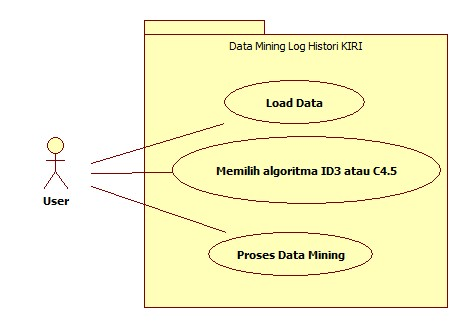
\includegraphics[scale=1]{Gambar/usecase.jpg}
\caption[Diagram \textsl{Use Case} Perangkat Lunak \textsl{Data Mining Log} Histori KIRI]{Diagram \textsl{Use Case} Perangkat Lunak \textsl{Data Mining Log} Histori KIRI} 
\label{fig:diagramUseCase}
\end{figure}

\begin{table}[H]
\caption{Skenario Melakukan \textsl{load} Data}
\begin{tabular}{|l|l|}
\hline
Nama           & Load data                                                       \\ \hline
Aktor          & \textit{User}                                                   \\ \hline
Deskripsi      & Memasukan alamat data yang akan dijadikan sebagai input program \\ \hline
Kondisi awal   & \textsl{Textbox} belum terisi                                   \\ \hline
Kondisi akhir  & \textsl{Textbox} sudah terisi dengan alamat data                \\ \hline
Skenario utama & \textit{User} memasukan alamat data pada textbox                \\ \hline
Eksespi        & Data tidak ditemukan                                            \\ \hline
\end{tabular}
\end{table}

\begin{table}[H]
\caption{Skenario Melakukan \textsl{Data Mining}}
\begin{tabular}{|l|l|}
\hline
Nama           & Proses \textsl{Data Mining }                      								\\ \hline
Aktor          & \textit{User}                                 										\\ \hline
Deskripsi      & Menekan tombol proses pada \textsl{interface}       					    \\ \hline
Kondisi awal   & \textsl{Textbox} belum terisi                          					\\ \hline
Kondisi akhir  & \textsl{Textbox} sudah terisi dengan hasil \textsl{data mining}  \\ \hline
Skenario utama & \textit{User} menekan tombol proses         										  \\ \hline
Eksespi        & Data tidak ditemukan atau data tidak dapat diproses    		  	  \\ \hline
\end{tabular}
\end{table}

\begin{table}[H]
\caption{Skenario Memilih Algoritma yang Akan Digunakan}
\begin{tabular}{|l|l|}
\hline
Nama           & Memilih algoritma ID3 atau C4.5                     \\ \hline
Aktor          & \textit{User}                                       \\ \hline
Deskripsi      & User memilih algoritma yang akan dipakai            \\ \hline
Kondisi awal   & \textsl{Radiobutton} terpilih pada ID3              \\ \hline
Kondisi akhir  & \textsl{Radiobutton} terpilih pada ID3 atau C4.5    \\ \hline
Skenario utama & \textit{User} memilih algoritma yang akan digunakan \\ \hline
Eksespi        & Tidak ada																					 \\ \hline
\end{tabular}
\end{table}


\subsection{Diagram kelas Perangkat Lunak \textsl{Data Mining Log} Histori KIRI}

Pembuatan diagram \textsl{class} untuk memenuhi semua tujuan dari diagram \textsl{use case} dan skenario terdapat pada gambar \ref{fig:classDiagram}.

\begin{figure}[h]
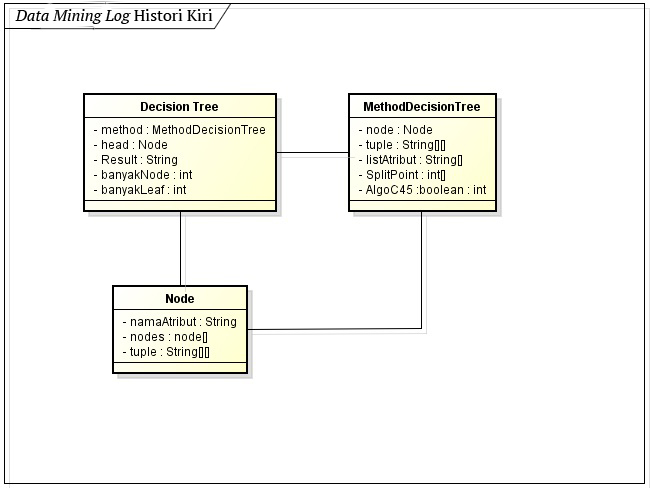
\includegraphics[scale=0.8]{Gambar/classdiagram.jpg}
\caption[Diagram \textsl{Class} Perangkat Lunak \textsl{Data Mining Log} Histori KIRI]{Diagram \textsl{Class} Perangkat Lunak \textsl{Data Mining Log} Histori KIRI} 
\label{fig:classDiagram}
\end{figure}

Berikut deskripsi kelas diagram \textsl{class}:
\begin{itemize}
	\item \textsl{DecisionTree}, merupakan kelas utama yang akan menjalankan algoritma pembuatan pohon
	\item \textsl{MethodDecisionTree}, merupakan kelas yang menjalankan algoritma pemilihan atribut untuk pembuatan pohon (pada penelitian ini, algoritma yang dapat dipilih adalah ID3 dan C4.5)
	\item \textsl{Node}, merupakan kelas yang digunakan sebagai struktur data untuk \textsl{decision tree}
\end{itemize}
	
















}{}
\ifdefstring{\vbabd}{1}{\chapter{Perancangan Perangkat Lunak}

Bab ini berisi tentang penjelasan perancangan perangkat lunak untuk melakukan proses \textsl{data mining} sesuai analisa yang sudah dibahas pada bab 3.

\section{Perancangan Perangkat Lunak}

\subsection{Perancangan Kelas}
Agar perangkat lunak dapat menjalankan fungsi yang sudah dibahas pada pemodelan fungsi di bab 3, maka pada subbab ini akan dibahas rancangan kelas dan \textsl{method} yang akan dibuat.

\begin{itemize}
	\item Kelas Controller, merupakan kelas untuk mengatur view dan modul ketika program dijalankan.
	\begin{itemize}
		\item Method
		\begin{itemize}
			\item public controller(), merupakan konstruktor dari kelas controller.
			\item public void startMining(String inputFilePath, String miningAlgo, JLabel label, JTextArea textArea), merupakan method untuk menjalankan modul-modul yang melakukan \textsl{data mining} dan membuat \textsl{decision tree} dari data yang menjadi masukan program.
			\item public static void main(String[] args), merupakan method main untuk menjalankan program.		
		\end{itemize}	
	\end{itemize}
	
	
	\item Kelas View, merupakan kelas untuk mengatur desain antar muka.
	\begin{itemize}
		\item Atribut
		\begin{itemize}
			\item ButtonGroup buttonGroup, digunakan untuk mengelompokkan jRadioButton.
			\item JButton buttonStart, merupakan sebuah tombol yang dapat memanggil method buttonStartActionPerformed() bila diklik.
			\item JButton buttonBrowse, merupakan sebuah tombol yang dapat memanggil method buttonBrowseActionPerformed() bila diklik.
			\item JLabel judul, merupakan sebuah label yang berisi judul dari aplikasi ini.
			\item JLabel labelFileData, merupakan label untuk menunjukkan bagian pemilihan file data \textsl{path}.
			\item JLabel labelPemilihanMethod, merupakan label untuk menunjukkan bagian pemilihan method.
			\item JLabel labelHasil, merupakan label untuk menunjukkan bagian hasil program.
			\item JLabel labelKeterangan, merupakan label untuk menunjukkan keterangan dari program.
			\item JRadioButton radioButtonId3, merupakan \textsl{radio button} yang menunjukkan bahwa user memilih method ID3 atau tidak.
			\item JRadiioButton radioButtonJ48, merupakan \textsl{radio button} yang menunjukkan bahwa user memilih method J48 atau tidak.
			\item JScrollPanel scrollPanel, merupakan variabel yang digunakan untuk mengaktifkan fungsi scroll pada JTextArea hasil.
			\item JTextArea hasil, merupakan sebuah JTextArea yang digunakan untuk menunjukkan hasil \textsl{data mining} dari program.
			\item JTextField textFieldFilePath, digunakan untuk melakukan \textsl{input path file }baik dilakukan secara manual atau melalui tombol \textsl{browse}.
			\item Controller cont, digunakan untuk memanggil \textsl{method} startMining ketika tombol buttonStart diklik.
		\end{itemize}
		\item Method
		\begin{itemize}
			\item public void buttonBrowseActionPerformed(java.awt.event.ActionEvent evt), digunakan untuk membuat jFileChooser yang berfungsi untuk memilih file dan mendapatkan \textsl{file path} dari file yang dipilih dan memasukkan \textsl{string }tersebut ke textFieldFilePath.
			\item public void buttonStartActionPerformed(java.awt.event.ActionEvent evt), digunakan untuk mengambil String dari textFieldFilePath serta method yang dipilih pada jRadioButton (Id3 atau J48) kemudian memanggil method startMining dengan masukan kedua file tersebut, label dan textArea.
		\end{itemize}
	\end{itemize}

	\item Kelas CSVReader, merupakan kelas yang memiliki method untuk membaca file dengan format CSV.
	\begin{itemize}
		\item Atribut
		\begin{itemize}
			\item ArrayList<String[]> data, digunakan untuk menyimpan isi dari file CSV yang sudah dibaca.
			\item int banyakAtribut, digunakan untuk menyimpan banyak atribut yang akan dibaca oleh CSV.
		\end{itemize}
		\item Method
		\begin{itemize}
			\item public CSVReader(), merupakan konstruktor dari kelas CSVReader.
			\item public void setEmpty, merupakan method untuk menghapus isi variabel data.
			\item public ArrayList readCSV(String file), digunakan untuk membaca file CSV.
			\item public ArrayList getData(), digunakan untuk mendapatkan variabel data.
			\item public void setData(ArrayList data), digunakan untuk mengganti nilai variabel data sesuai dengan parameter.
			\item public int getBanyakAtribut(), digunakan untuk mendapatkan nilai variabel banyakAtribut.
			\item public void setBanyakAtribut(int banyakAtribut), digunakan untuk menggati nilai variabel banyakAtribut sesuai dengan parameter.
		\end{itemize}
	\end{itemize}

	\item Kelas ProcessingData, merupakan kelas yang memiliki method untuk melakukan \textsl{preprocessing data}.
	\begin{itemize}
		\item Method
		\begin{itemize}
			\item public ProcessingData(), merupakan konstruktor dari kelas ProcessingData.
			\item public void processSorting(ArrayList array, ArrayList data, String action), digunakan untuk memilah arraylist sehingga arraylist tersebut hanya berisi \textsl{action} yang diinginkan saja (pada penelitian ini, \textsl{action} yang diharapkan adalah FINDROUTE). Hasil pilah akan disimpan pada varibel array dari parameter method sehingga tidak diperlukan return value.
			\item public ArrayList preprocessingData(ArrayList<String[]> data), Digunakan untuk melakukan tahap \textsl{preprocessing data} seperti yang sudah dijelaskan pada pemodelan data di bab 3. Tujuan dari fungsi ini adalah mendapatkan nilai waktu yang sudah diubah menjadi GMT+7 dan sudah dikelompokkan menjadi jam, hari, bulan, dan tahun serta mengetahui klasifikasi kelas dari untuk setiap \textsl{record} dengan menghitung jarak dari titik keberangkatan terhadap titik pusat Bandung dan titik tujuan terhadap titik pusat Bandung.
			\item public int KlasifikasiKelas(double jarakKeberangkatan, double jarakTujuan), Digunakan untuk menentukan kelas dari hasil jarak titik keberangkatan dengan titik pusat Bandung dan titik tujuan dengan titik pusat Bandung. 
		\end{itemize}
	\end{itemize}

	\item Kelas DecisionTree, merupakan kelas yang memiliki method untuk membuat \textsl{decision tree} dan menghitung \textsl{confident} dari pohon yang sudah dihasilkan.
	\begin{itemize}
		\item Atribut
		\begin{itemize}
			\item Classifier tree, digunakan untuk menyimpan \textsl{decision tree} yang sudah dihasilkan.
		\end{itemize}
		\item Method
		\begin{itemize}
			\item public DecisionTree(), merupakan konstruktor untuk kelas DecisionTree.
			\item public double calculateConfident(Instances data), digunakan untuk mendapatkan nilai confident dari \textsl{decision tree} yang dihasilkan.
			\item public String id3(Instances data), digunakan untuk membuat \textsl{decision tree} dengan menggunakan metode ID3 dari API Weka.
			\item public String j48(Instances data), digunakan untuk membuat \textsl{decision tree} dengan menggunakan metode J48 dari API Weka.
		\end{itemize}
	\end{itemize}

	\item Kelas Dot Converter, merupakan kelas yang memiliki method untuk mengubah \textsl{string} yang merupakan hasil dari kelas DecissionTree (yaitu, \textsl{decision tree} dalam bentuk string) menjadi bahasa dot yang siap dijadikan masukan untuk graphviz.
	\begin{itemize}
		\item Method
		\begin{itemize}
			\item public String convert(String data, String miningAlgo, String nodeName), Digunakan untuk mengubah nilai string yang sudah diperoleh dari kelas DecisionTree menjadi bahasa DOT untuk membuat visualisasi dengan menggunakan graphviz.
		\end{itemize}
	\end{itemize}
\end{itemize}
	
	Pada kelas ProcessingData, nilai data waktu perlu diganti menjadi GMT+7 dan perlu menghitung jarak antar dua titik. Maka dari itu, akan dibuat dua kelas tambahan untuk melakukan kedua hal tersebut, yaitu TimezoneConverter dan DistanceHaversine.
	
\begin{itemize}
	\item Kelas TimezoneConverter, merupakan kelas yang memiliki \textsl{method} untuk mengubah waktu dari UTC menjadi GMT+7
	\begin{itemize}
		\item Method
		\begin{itemize}
			\item public static String convertToGMT7(String date), digunakan untuk mengubah waktu dari UTC menjadi GMT+7.
		\end{itemize}
	\end{itemize}

	\item Kelas DistanceHaversine, kelas yang memiliki \textsl{method} untuk menghitung jarak dua titik di bumi.
	\begin{itemize}
		\item Atribut
		\begin{itemize}
			\item double r, digunakan untuk menyimpan nilai radius dari bumi.
		\end{itemize}
		\item Method
		\begin{itemize}
			\item public double calculateDistance(double latitude1, double longitude1, double latitude2, double longitude2), Digunakan untuk menghitung jarak dari dua titik (latitude dan longitude).
		\end{itemize}
	\end{itemize}
\end{itemize}

	Setelah melakukan penelitian tentang API Weka, diperoleh bahwa input untuk membuat \textsl{decision tree} merupakan kelas Instances dari API Weka. Selain itu, diperlukan juga pengecekkan untuk hasil dari kelas tersebut, apakah sudah sesuai dengan aplikasi Weka atau belum (karena menggunakan API Weka, seharusnya \textsl{decision tree} yang dihasilkan sama). Oleh karena itu, akan ditambahkan kelas ArffIO yang berfungsi untuk menulis dan membaca data dengan format arff, sehingga ketika program melakukan \textsl{data mining}, program akan menghasilkan file dengan format .arff yang dapat dibaca oleh aplikasi Weka untuk melakukan pengetesan. Karena kita sudah memiliki file .arff tersebut, ada baiknya jika menggunakan fungsi membaca arff dari API Weka yang menghasilkan \textsl{return value} berupa kelas Instances yang dapat digunakan untuk membuat \textsl{decision tree}.

\begin{itemize}
	\item Kelas ArffIO, merupakan kelas yang berfungsi untuk melakukan penyimpanan dan membaca data dengan format arff.
	\begin{itemize}
		\item Method
		\begin{itemize}
			\item public ArffIO, merupakan konstruktor dari kelas ArffIO.
			\item public void writeArffIO(String name, ArrayList<int[]> data), digunakan untuk menulis file .arff sesuai data pada parameter.
			\item public Instances arffRead(String name), digunakan untuk membaca file .arff dengan menggunakan \textsl{method} dari API Weka.
		\end{itemize}
	\end{itemize}
\end{itemize}

Ketika mulai merancang \textsl{method} convert yang berada di kelas DotConverter, akan lebih mudah jika dirancang menjadi rekursif. Karena data yang diolah pada \textsl{method}
tersebut cukup banyak dan diperlukan nama yang berbeda pada setiap node yang akan ditulis pada DOT, maka perlu ditambah kelas yang berfungsi untuk struktur data pada kelas tersebut, yaitu SDForConvertTree.

\begin{itemize}
	\item kelas SDForConvertTree, kelas yang berfungsi untuk menyimpan data yang dibutuhkan untuk mengubah String hasil dari kelas DecisionTree menjadi bahasa DOT.
	\begin{itemize}
		\item Atribut
		\begin{itemize}
			\item String[] data, digunakan untuk menyimpan nama-nama atribut yang akan diubah ke dalam bahasa DOT.
			\item int[] count, digunakan untuk menghitung penggunaan nama setiap atribut sehingga dapat menghasilkan nama node yang berbeda untuk setiap atribut.
		\end{itemize}
		\item Method
		\begin{itemize}
			\item public SDForConvertTree(String[] data), merupakan konstruktor untuk kelas ini dan akan melakukan inisialisasi data pada atribut dengan nilai data pada parameter serta melakukan inisialisasi nilai variabel count dengan 0.
			\item public void setData(String data, index int), digunakan untuk mengubah nilai data pada index tertentu.
			\item public String[] getData(), digunakan untuk mendapatkan nilai atribut data.
			\item public String getData(int index), digunakan untuk mendapatkan nilai data pada index tertentu.
			\item public void setCount(int count, int index), digunakan untuk mengubah nilai count pada index tertentu.
			\item public int getCount(int index), digunakan untuk mendapatkan nilai count pada index tertentu.
			\item public boolean hasNext(), digunakan untuk mengecek apakah varibel data masih ada atau tidak.
			\item public void buangArrayPertama(), digunakan untuk membuang nilai array yang pertama (index ke-0).
			\item public String getDataNumber(String atribut), digunakan untuk mendapatkan angka pada nama atribut tertentu untuk membuat nama node pada kelas DotConverter agar semua nama node berbeda.
		\end{itemize}
	\end{itemize}
\end{itemize}

Setelah melakukan \textsl{convert} dari \textsl{string} hasil dari \textsl{method} pembuatan \textsl{decision tree} dari API Weka ke bahasa Dot, maka diperlukan pemanggilan fungsi dot yang terdapat pada graphviz. Cara memanggilan fungsi tersebut yaitu dengan menggunakan \textsl{command prompt}. Maka dari itu, akan diperlukan kelas yang memiliki \textsl{method} untuk memanggil \textsl{command prompt} dan menjalankan fungsi dot tersebut, yaitu kelas CMD.


\begin{itemize}
	\item kelas CMD, merupakan kelas yang digunakan untuk memanggil \textsl{command prompt}.
	\begin{itemize}
		\item Method
		\begin{itemize}
			\item public static void makeJpgUsingDotCommand(), digunakan untuk memanggil \textsl{command prompt} dan menjalankan fungsi dot dan menghasil gambar visualisasi grafik sesuai dengan file yang menjadi masukan fungsi tersebut.
		\end{itemize}
	\end{itemize}
\end{itemize}

Karena cara yang untuk memanggil fungsi dot adalah \textsl{command prompt}, maka hasil dari \textsl{method} convert harus disimpan dalam bentuk file text agar dapat dibaca oleh \textsl{command prompt}.

Dari perancangan kelas dan \textsl{method} yang sudah dilakukan, maka akan diperoleh diagram kelas seperti pada \ref{fig:classDiagram2}

\begin{figure}[H]
\includegraphics[scale=0.5, angle =90]{Gambar/classdiagram2.jpg}
\caption[Diagram \textsl{Class} Perangkat Lunak \textsl{Data Mining Log} Histori KIRI]{Diagram \textsl{Class} Perangkat Lunak \textsl{Data Mining Log} Histori KIRI} 
\label{fig:classDiagram2}
\end{figure}

\subsection{Sequence Diagram}

Pada subbab ini, akan dijelaskan alur program dengan menggunakan \textsl{sequence diagram} pada \ref{fig:sequenceDiagram}.

Pertama, program akan menampilkan desain antar muka yang dihasilkan oleh kelas View. Kemudian user akan menulis \textsl{file path} atau memilih (dengan menggunakan tombol \textsl{browse}) \textsl{input} file pada JTextField serta memilih metode pembuatan \textsl{decision tree} (tahap  pertama). Setelah memilih file dan metode, user akan menekan tombol start, dan kelas View akan memanggil \textsl{method} startMining dari kelas controller (tahap 3-4).

Kelas Controller akan mengakses file sesuai dengan masukan \textsl{file path} dengan memanggil \textsl{method} readCSV dari kelas CSVReader dan mendapat nilai kembalian berupa arraylist (tahap 5-6). Setelah mendapatkan data dari file CSV yang dipilih, data tersebut akan dipilah dan menggambil \textsl{record} dengan \textsl{action} FINDROUTE dengan cara memanggil \textsl{method} processSorting pada kelas ProcessingData dan mengembalikan ArrayList dengan data yang sudah dipilah (tahap 7-8). Kemudian data tersebut akan dilakukan \textsl{preprocessing data} dengan cara memanggil \textsl{method} preprocessingData dari kelas ProcessingData(tahap 9).

Ketika \textsl{method} preprocessingData dijalankan, perlu mengubah nilai waktu dari UTC menjadi GMT+7 dengan cara memanggil \textsl{method} convertGMT7 dari kelas TimezoneConverter dan mengembalikan nilai bertipe Date (tahap 10-11). Setelah nilai waktu diubah, diperlukan perhitungan jarak antara dua titik dengan cara memanggil \textsl{method} calculateDistance  dari kelas DistanceHaversine dan mengebalikan nilai double yang berisi jarak dari kedua titik(tahap 12-13). Kemudian diperlukan klasifikasi kelas dari jarak yang sudah dihasilkan dengan cara memanggil \textsl{method} klasifikasiKelas dari kelas ProcessingData (tahap 14-15). Kemudian semua data yang sudah diproses akan dikembalikan dalam bentuk ArrayList(tahap 16).

Setelah didapat data yang sudah dilakukan \textsl{preprocessing data}, data tersebut akan disimpan dengan format arff dengan cara memanggi \textsl{method} writeArff pada kelas ArffIO(tahap 17). Setelah disimpan, diperlukan mengambil data dari file arff yang sudah disimpan untuk mendapatkan data dengan tipe Instance dengan cara memanggil \textsl{method}readArff(tahap 18-19).

Kemudian program akan membuat \textsl{decision tree} dengan cara memanggil \textsl{method} id3 atau j48 pada kelas DecisionTree dan mengembalikan \textsl{decision tree} dalam bentuk \textsl{String}(tahap 20-21). Setelah \textsl{decision tree} dibuat, perlu dicari nilai \textsl{confident} yang diperoleh dari \textsl{decision tree} tersebut dengan cara memanggil \textsl{method} calculateConfident dan nilai \textsl{confident} yang dihasilkan dikembalikan dalam bentuk double(tahap 22-23).

Tahap selanjutnya adalah mengubah nilai String yang diperoleh dari \textsl{method} id3 atau j48 menjadi bahasa DOT dengan cara memanggil \textsl{method} convert pada kelas DotConverter dan akan mengembalikan nilai String(tahap 24-25). Setelah diperoleh hasil dari \textsl{method} convert, maka diperlukan \textsl{command prompt} untuk menghasilkan gambar grafik untuk melakukan visualisasi \textsl{decision tree} yang sudah dihasilkan(tahap 26-27).

Setelah gambar \textsl{decision tree} dihasilkan, maka \textsl{method} startMining akan membuat JFrame yang baru untuk memperlihatkan hasil gambar \textsl{decision tree} yang sudah diperoleh serta mengembalikan nilai String \textsl{decision tree} kepada kelas View yang akan ditampilkan di JTextArea(tahap 28-29).


\begin{figure}[H]
\includegraphics[scale=0.42, angle =90]{Gambar/sequenceDiagram.jpg}
\caption[Diagram \textsl{Class} Perangkat Lunak \textsl{Data Mining Log} Histori KIRI]{Diagram \textsl{Class} Perangkat Lunak \textsl{Data Mining Log} Histori KIRI} 
\label{fig:sequenceDiagram}
\end{figure}

\subsection{Perancangan Desain Antar Muka}

Pada subbab ini, akan diperlihatkan rancangan desain antar muka yang akan digunakan untuk program ini.

Aplikasi ini memiliki dua form untuk melakukan \textsl{data mining} dan membuat \textsl{decision tree}. Pada form pertama(dapat dilihat di \ref{fig:MU1}) disediakan JTextbox dan JButton yang digunakan untuk memilih file, JRadioButton yang digunakan untuk memilih metode pembuatan \textsl{decision tree}, JTextArea yang digunakan untuk memperlihatkan hasil \textsl{decision tree} yang diperoleh dalam bentuk String, serta JTextButton yang kedua (dengan label Start) yang digunakan untuk memulai proses \textsl{data mining}. Sedangkan form kedua, berisi gambar visualisasi \textsl{decision tree} yang sudah dihasilkan(dapat dilihat di \ref{fig:MU2}).
\begin{figure}[H]
\centering
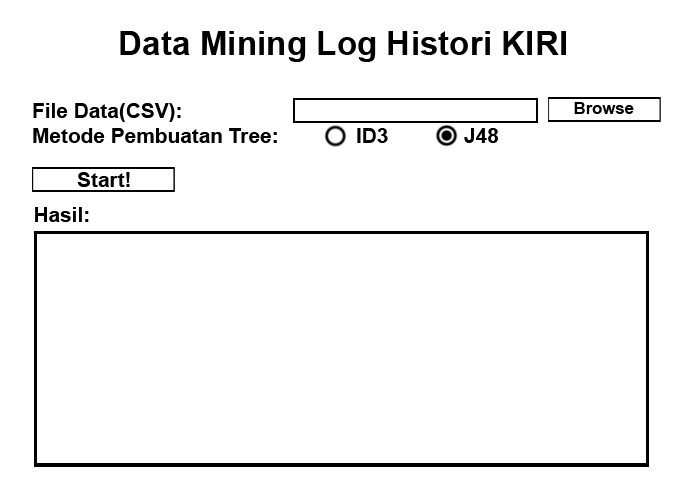
\includegraphics[scale=1.2]{Gambar/mockUp1.jpg}
\caption[Mock Up Form Pertama]{Mock Up Form Pertama} 
\label{fig:MU1}
\end{figure}

\begin{figure}[H]
\centering
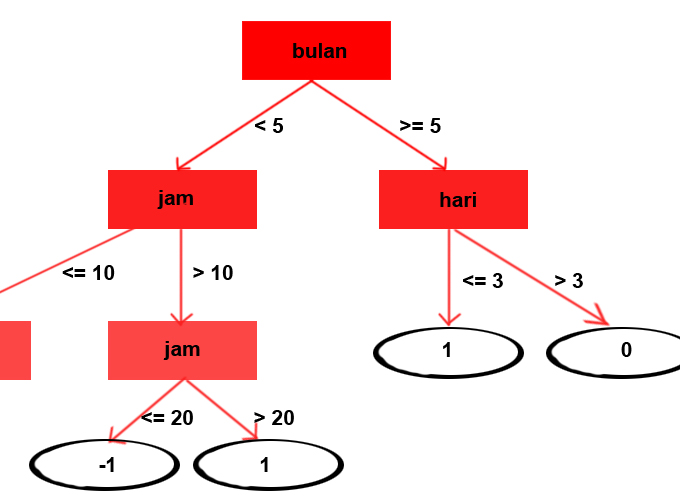
\includegraphics[scale=1.2]{Gambar/mockUp2.jpg}
\caption[Mock Up Form Kedua]{Mock Up Form Kedua} 
\label{fig:MU2}
\end{figure}}{}
\ifdefstring{\vbabe}{1}{\chapter{Implementasi Program dan Pengujian}

Pada bab ini, akan dijelaskan tentang lingkupan pembangunan, implementasi rancangan antarmuka, serta pengujian secara fungsional dan experimental pada aplikasi \textsl{data mining}.

\section{Lingkungan Pembangunan}
Lingkungan perangkat lunak dan perangkat keras yang digunakan untuk membangun dan menguji aplikasi \textsl{data mining} ini adalah:

\begin{enumerate}
	\item CPU
	\begin{itemize}
		\item Prosesor: Intel(R) Core(TM) i7, 1.60 GHz
		\item RAM: 6 GB
		\item VGA: NVDIA GeForce GT 330M
		\item Hardisk: 300 GB
	\end{itemize}
	\item Sistem operasi: Windows 7 Professional
	\item Platform: NetBeans: IDE 8.0
\end{enumerate}

\section{Hasil Tampilan Antarmuka}
Pada aplikasi \textsl{data mining} ini, terdapat dua form. Form pertama berfungsi untuk memilih file CSV yang akan dilakukan \textsl{data mining}, memilih metode pembuatan \textsl{decision tree}, serta menunjukkan hasil \textsl{decision tree} yang dihasilkan dalam bentuk String. Sedangkan untuk form kedua, berfungsi untuk memvisualisasikan \textsl{decision tree} yang sudah diperoleh dalam bentuk gambar.

TextField yang pertama berfungsi untuk mengisi alamat file CSV yang akan dilakukan \textsl{data mining}. RadioButton berfungsi untuk memilih metode manakah yang akan digunakan untuk membuat \textsl{decision tree}, sedangkan TextArea digunakan untuk memperlihatkan hasil \textsl{decision tree} dalam bentuk String. Tampilan awal aplikasi dapat dilihat di \ref{fig:GUI1}.

\begin{figure}[H]
\centering
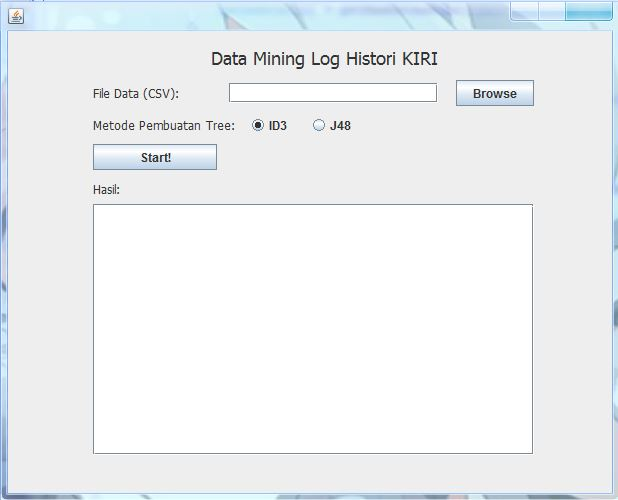
\includegraphics[scale=0.7]{Gambar/GUI1.jpg}
\caption[Tampilan Form Awal Aplikasi \textsl{Data Mining}]{Tampilan Form Awal Aplikasi \textsl{Data Mining}} 
\label{fig:GUI1}
\end{figure}

Terdapat dua cara untuk mengisi TextField, yaitu ditulis secara manual alamat file CSV atau dengan cara mengklik tombol button browse dan memilih file CSV pada FileSelector. Tampilan memilih file CSV dapat dilihat pada gambar \ref{fig:GUI2} dan tampilan setelah memilih file CSV dapat dilihat pada gambar \ref{fig:GUI3}.

\begin{figure}[H]
\centering
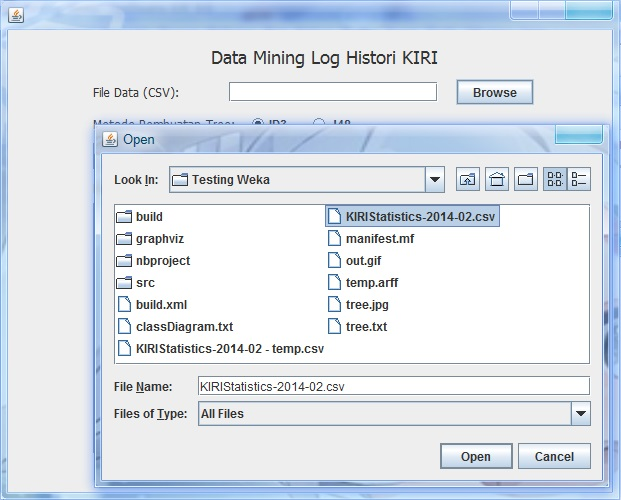
\includegraphics[scale=0.7]{Gambar/GUI2.jpg}
\caption[Tampilan FileSelector untuk Memilih File CSV]{Tampilan FileSelector untuk Memilih File CSV} 
\label{fig:GUI2}
\end{figure}

\begin{figure}[H]
\centering
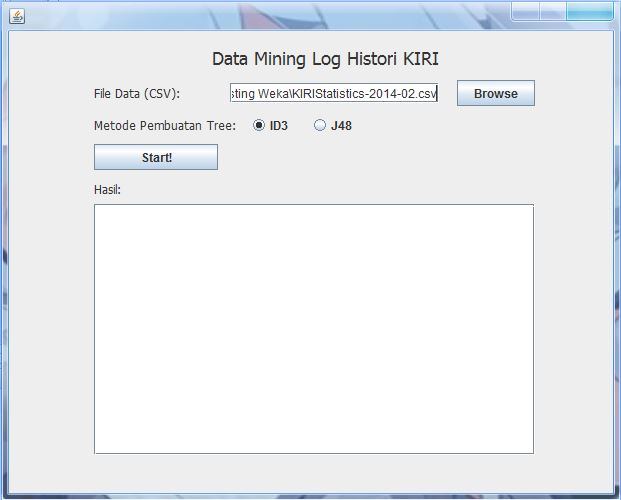
\includegraphics[scale=0.7]{Gambar/GUI3.jpg}
\caption[Tampilan Form setelah Memilih File CSV]{Tampilan Form setelah Memilih File CSV} 
\label{fig:GUI3}
\end{figure}

Setelah alamat file CSV diisi, hal selanjutnya yang dilakukan adalah memilih metode pembuatan \textsl{decision tree} pada RadioButton. RadioButton akan memilih metode ID3 jika \textsl{setting} ini tidak diubah. Tampilan tersebut dapat dilihat di gambar \ref{fig:GUI3and4}.

\begin{figure}[H]
\centering
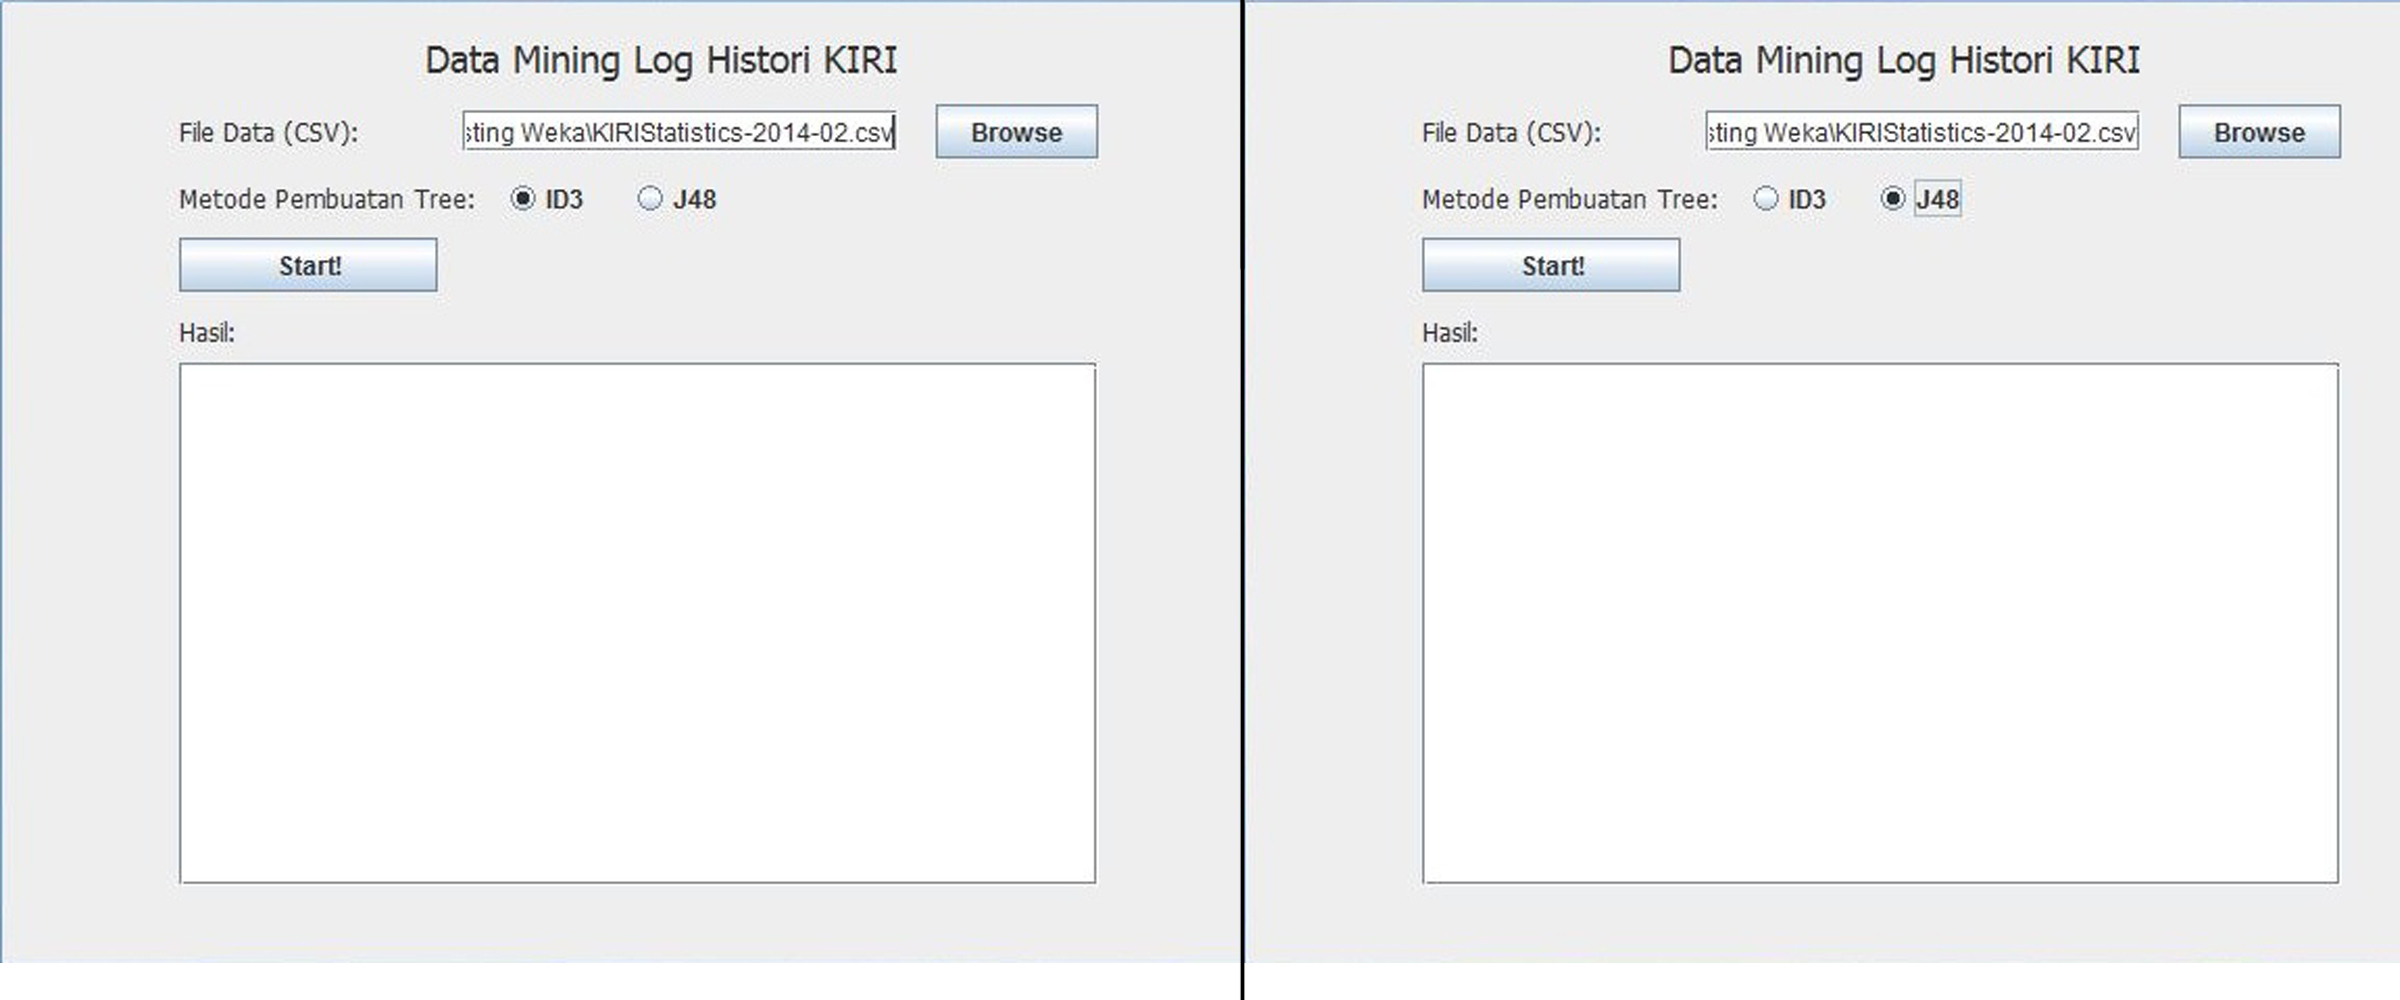
\includegraphics[scale=0.7]{Gambar/GUI3and4.jpg}
\caption[Tampilan Form Pemilihan Metode Pembuatan \textsl{Decision Tree}]{Tampilan Form Pemilihan Metode Pembuatan \textsl{Decision Tree}. Gambar a merupakan kondisi tampilan ketika metode ID3 dipilih sedangkan gambar b merupakan kondisi tampilan ketika metode J48 dipilih.} 
\label{fig:GUI3and4}
\end{figure}

Kemudian, tombol start diklik lalu program akan melakukan proses \textsl{data mining}. Setelah selesai, maka program akan menunjukkan hasil \textsl{data mining} dalam bentuk String pada TextArea dan dalam bentuk gambar pada form kedua. Tampilan akhir dari aplikasi serta form kedua dapat dilihat di gambar \ref{fig:GUI5}.

\begin{figure}[H]
\centering
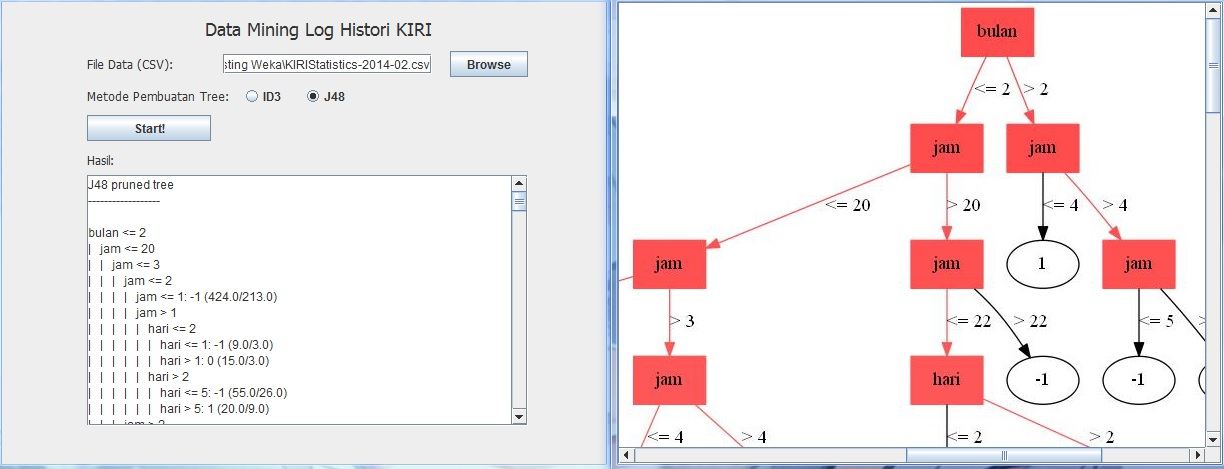
\includegraphics[scale=0.5]{Gambar/GUI5.jpg}
\caption[Tampilan Form Menampilkan Hasil \textsl{Data Mining}]{Tampilan Form Menampilkan Hasil \textsl{Data Mining}} 
\label{fig:GUI5}
\end{figure}

\section{Pengujian Aplikasi \textsl{Data Mining}}

\subsection{Rancangan Pengujian}

Dalam pengujian aplikasi \textsl{data mining} ini, akan digunakan teknik pengujian \textsl{black box}. Pengujian yang akan dilakukan:
\begin{enumerate}
	\item Pengujian \textsl{method} utama untuk mencapai tujuan dari aplikasi \textsl{data mining} ini. Terdapat beberapa \textsl{method} yang perlu diuji, yaitu
	\begin{enumerate}
		\item \textsl{method} untuk membaca file CSV
		\item \textsl{method} untuk melakukan \textsl{preprocessing data}
		\item \textsl{method} untuk membuat \textsl{decision tree}
		\item \textsl{method} untuk mengubah \textsl{decision tree} dalam bentuk String menjadi bahasa DOT
	\end{enumerate}
	\item Kebenaran perangkat lunak hanya dilihat pada hasil keluaran program atau kondisi masukan yang diberikan tanpa melihat bagaimana proses untuk mendapatkan keluaran tersebut.
	\item Dari keluaran yang dihasilkan, kemampuan program untuk memenuhi kebutuhan pemakai dapat diukur dan dapat diketahui kesalahan jika ada.
\end{enumerate}


\subsection{Hasil Pengujian}

Dibuat sebuah \textsl{test case} yang berisi 20 data \textsl{log} histori KIRI dengan data pada tabel \ref{table:dataTestCase}

\begin{table}[H]
\rotatebox{90}{
\begin{tabular}{|l|l|l|l|l|}
\hline
\textbf{logId} & \textbf{APIKey}  & \textbf{Timestamp (UTC)} & \textbf{Action} & \textbf{AdditionalData}                                        \\ \hline
114055         & E5D9904F0A8B4F99 & 2/1/2014 2:34            & FINDROUTE       & -6.88968,107.59632/-6.88461,107.61361/3                        \\ \hline
114056         & E5D9904F0A8B4F99 & 2/1/2014 2:34            & FINDROUTE       & -6.88968,107.59632/-6.88461,107.61361/3                        \\ \hline
114057         & E5D9904F0A8B4F99 & 2/1/2014 2:34            & FINDROUTE       & -6.88968,107.59632/-6.88461,107.61361/3                        \\ \hline
114058         & A44EB361A179A49E & 2/1/2014 2:35            & FINDROUTE       & -6.9112484,107.6275648/-6.875449306549391,107.60455314069986/1 \\ \hline
114059         & E5D9904F0A8B4F99 & 2/1/2014 2:37            & PAGELOAD        & /5.10.83.99/                                                   \\ \hline
114060         & A44EB361A179A49E & 2/1/2014 2:38            & SEARCHPLACE     & cimol\%2C+/10                                                  \\ \hline
114061         & A44EB361A179A49E & 2/1/2014 2:38            & FINDROUTE       & -6.8779112,107.612129/-6.92663,107.63644/1                     \\ \hline
114062         & A44EB361A179A49E & 2/1/2014 2:38            & SEARCHPLACE     & gedebage\%2C+/10                                               \\ \hline
114063         & A44EB361A179A49E & 2/1/2014 2:38            & SEARCHPLACE     & gedebage\%2C+cimol/10                                          \\ \hline
114064         & A44EB361A179A49E & 2/1/2014 2:39            & FINDROUTE       & -7.3275023,108.3614085/-6.93269,107.69734/1                    \\ \hline
114065         & A44EB361A179A49E & 2/1/2014 2:39            & WIDGETLOAD      & /66.249.77.219/                                                \\ \hline
114066         & A44EB361A179A49E & 2/1/2014 2:39            & FINDROUTE       & -6.863680050774415,107.5951399281621/-6.93269,107.69734/1      \\ \hline
114067         & A44EB361A179A49E & 2/1/2014 2:43            & FINDROUTE       & -6.9423325,107.7486968/-6.90112,107.60787/1                    \\ \hline
114068         & A44EB361A179A49E & 2/1/2014 2:43            & FINDROUTE       & -6.9423325,107.7486968/-6.88623,107.60821/1                    \\ \hline
114069         & A44EB361A179A49E & 2/1/2014 2:44            & FINDROUTE       & -6.9423062,107.7490084/-6.88623,107.60821/1                    \\ \hline
114070         & A44EB361A179A49E & 2/1/2014 2:45            & FINDROUTE       & -6.9072888,107.6143937/-6.90855,107.61082/1                    \\ \hline
114071         & A44EB361A179A49E & 2/1/2014 2:46            & FINDROUTE       & -6.9286306,107.6227444/-6.91708,107.60880/1                    \\ \hline
114072         & A44EB361A179A49E & 2/1/2014 2:46            & FINDROUTE       & -6.908639785445589,107.61091567575932/-6.90855,107.61082/1     \\ \hline
114073         & A44EB361A179A49E & 2/1/2014 2:47            & SEARCHPLACE     & hotel+harapan+i/10                                             \\ \hline
114074         & A44EB361A179A49E & 2/1/2014 2:47            & SEARCHPLACE     & hotel+harapan+ind/10                                           \\ \hline
\end{tabular}}
\caption{Data untuk \textsl{Test Case} Aplikasi \textsl{Data Mining}}
\label{table:dataTestCase}
\end{table}

Berikut hasil pengujian yang dilakukan dengan menggunakan data tersebut:
\begin{enumerate}
	\item Pengujian pertama: Membaca file CSV, data akan diambil oleh program dan dipilah, hanya record dengan \textsl{action} FINDROUTE yang akan diambil sedangkan yang lain akan dibuang. Berikut hasil dengan contoh data diatas dengan menggunakan sistem \textsl{debug} untuk melihat data yang diambil dari csv pada \ref{fig:Pengujian1} dan \ref{fig:Pengujian12}
	
	\begin{figure}[H]
	\centering
	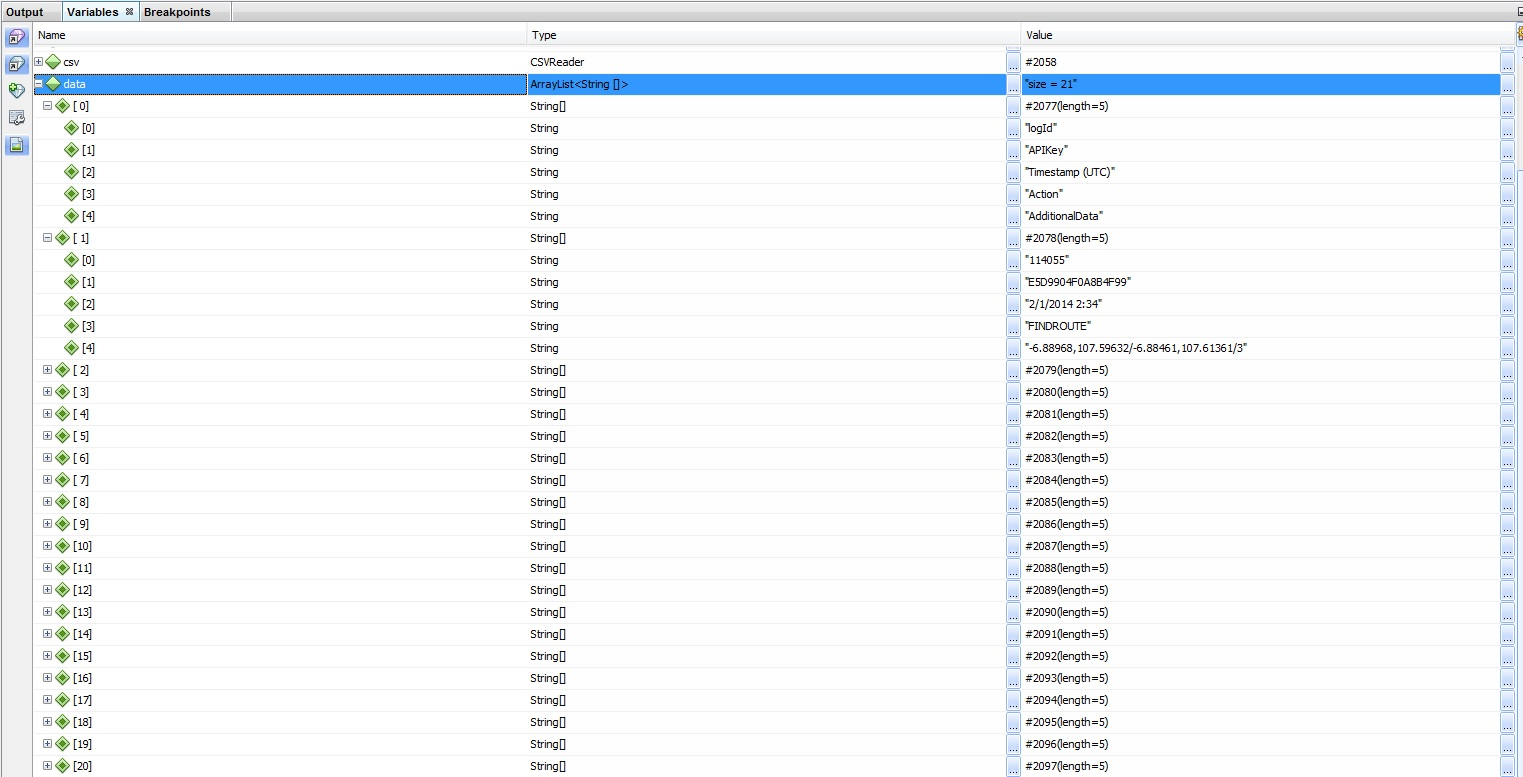
\includegraphics[scale=0.4]{Gambar/pengujian1.jpg}
	\caption[Pengujian Mengambil Data CSV]{Pengujian Mengambil Data CSV} 
	\label{fig:Pengujian1}
	\end{figure}

	\begin{figure}[H]
	\centering
	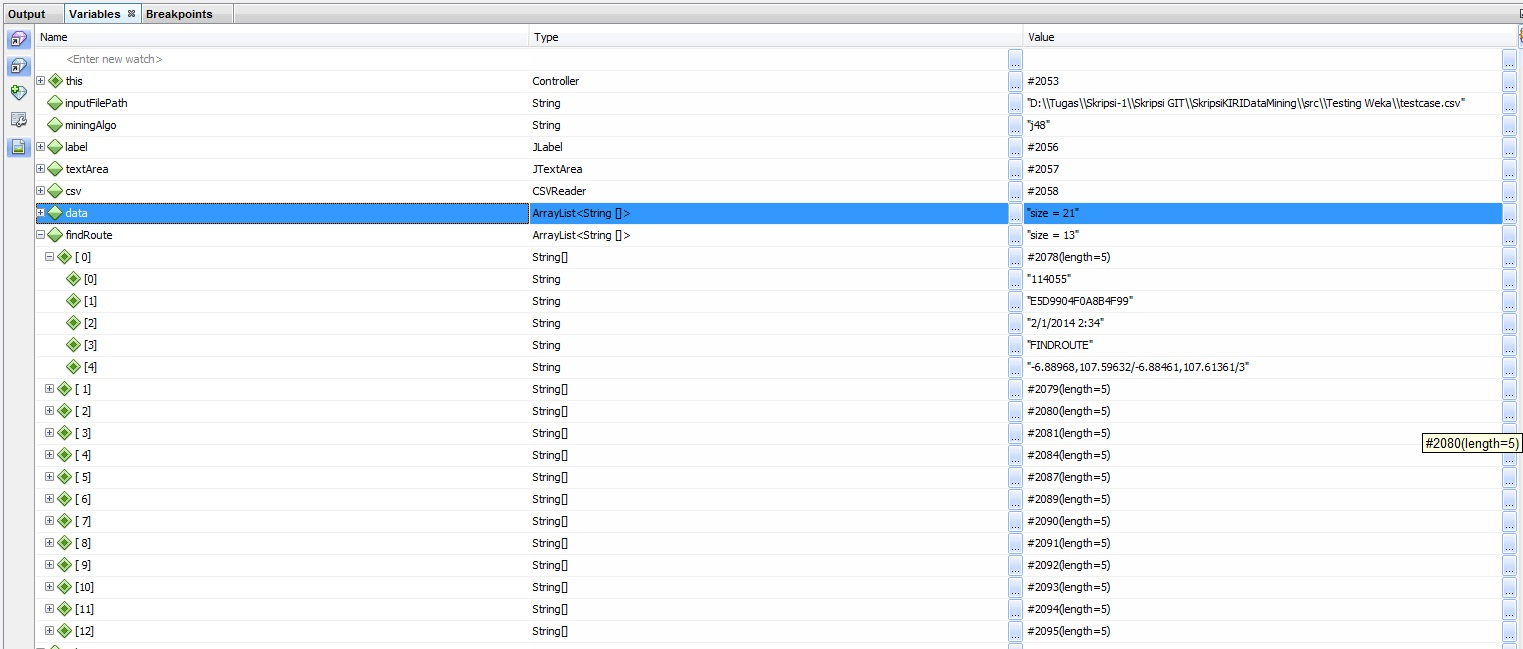
\includegraphics[scale=0.4]{Gambar/pengujian12.jpg}
	\caption[Pengujian Pemilahan Data CSV]{Pengujian Pemilahan Data CSV} 
	\label{fig:Pengujian12}
	\end{figure}

	Gambar pertama memperlihatkan bahwa data pertama yang diperoleh 21 array String dengan array pertama adalah atributnya sedangkan array selanjutnya adalah isi data yang diperoleh. Pada gambar kedua, terdapat 13 array String dimana semua array tersebut merupakan record dengan nilai \textsl{action} FINDROUTE. Dengan demikian, pengujian membaca CSV berhasil dilakukan.

	\item Pengujian kedua: Melakukan \textsl{preprocessing data}, data yang digunakan adalah 13 array String yang sudah diperoleh dari pengujian pertama. Pengujian dilakukan dengan melakukan pengecekan data dengan menggunakan weka untuk melihat data yang sudah dihasilkan, dapat dilihat pada \ref{fig:Pengujian214} dan \ref{fig:Pengujian25} 
	
	\begin{figure}[H]
	\centering
	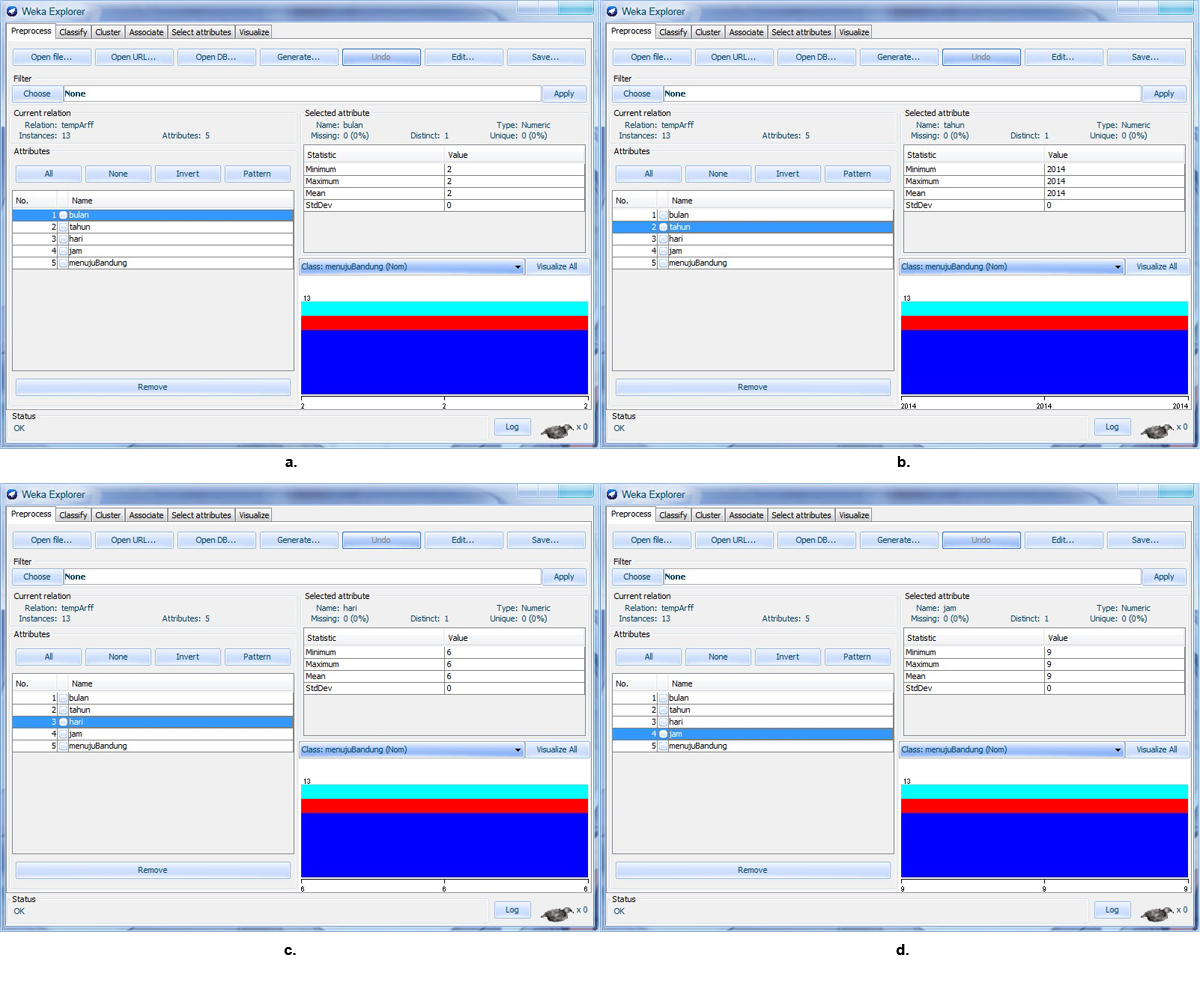
\includegraphics[scale=0.4]{Gambar/pengujian214.jpg}
	\caption[Pengujian \textsl{Preprocessing Data}]{Pengujian \textsl{Preprocessing Data}. Gambar a menunjukkan nilai pada atribut bulan. Gambar b menunjukkan nilai pada atribut tahun. Gambar c menunjukkan nilai pada atribut hari. Gambar d menunjukkan nilai pada atribut jam.} 
	\label{fig:Pengujian214}
	\end{figure}
	
	\begin{figure}[H]
	\centering
	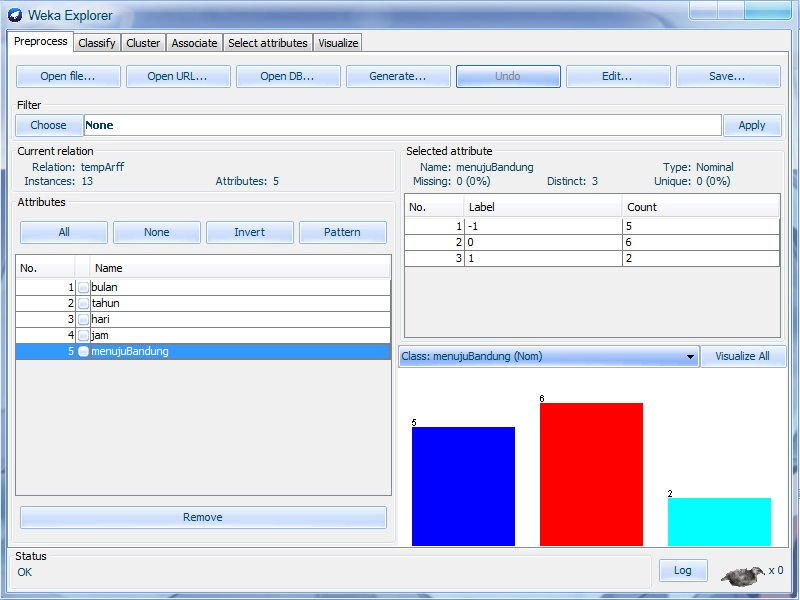
\includegraphics[scale=0.4]{Gambar/pengujian25.jpg}
	\caption[Pengujian \textsl{Preprocessing Data} untuk Klasifikasi Data]{Pengujian \textsl{Preprocessing Data} untuk Klasifikasi Data} 
	\label{fig:Pengujian25}
	\end{figure}

	Terdapat dua tahap penting pada \textsl{prerpocessing data}, yaitu pengubahan waktu dari UTC menjadi GMT+7 dan klasifikasi area. Pada tahap pengubahan waktu dari UTC menjadi GMT+7, pada gambar \ref{fig:Pengujian214} d, atribut jam yang dimiliki menjadi bernilai sembilan karena pada testcase, nilai atribut jam adalah dua. Pada tahap klasifikasi area, dapat dilihat pada tabel \ref{table:PenentuanAreaDanKlasifikasi}
	
	\begin{table}[H]
	\centering
	\begin{tabular}{|l|l|l|}
	\hline
	\multicolumn{1}{|c|}{\textbf{Region Keberangkatan}} & \multicolumn{1}{c|}{\textbf{Region Tujuan}} & \multicolumn{1}{c|}{\textbf{Hasil Klasifikasi}} \\ \hline
	3                                                   & 3                                           & 0                                               \\ \hline
	3                                                   & 3                                           & 0                                               \\ \hline
	3                                                   & 3                                           & 0                                               \\ \hline
	3                                                   & 4                                           & 1                                               \\ \hline
	4                                                   & 4                                           & 0                                               \\ \hline
	11                                                  & 10                                          & -1                                              \\ \hline
	5                                                   & 10                                          & 1                                               \\ \hline
	11                                                  & 1                                           & -1                                              \\ \hline
	11                                                  & 3                                           & -1                                              \\ \hline
	11                                                  & 3                                           & -1                                              \\ \hline
	1                                                   & 1                                           & 0                                               \\ \hline
	2                                                   & 0                                           & -1                                              \\ \hline
	1                                                   & 1                                           & 0                                               \\ \hline
	\end{tabular}
	\caption{Hasil Penentuan area dan Klasifikasi}
	\label{table:PenentuanAreaDanKlasifikasi}
	\end{table}
	
	Terdapat lima data dengan klasifikasi -1, enam data dengan klasifikasi 0, dan 2 data dengan klasifikasi 1. Dari kedua hasil tersebut, dapat disimpulkan bahwa tahap \textsl{preprocessing data} sudah berjalan dengan baik.
	
	\item Pengujian ketiga: Membuat \textsl{decision tree}, akan dilakukan perbandingan antara hasil dari program dengan hasil dari weka, dapat dilihat pada gambar \ref{fig:Pengujian31} dan 
	\ref{fig:Pengujian32}.
	
	\begin{figure}[H]
	\centering
	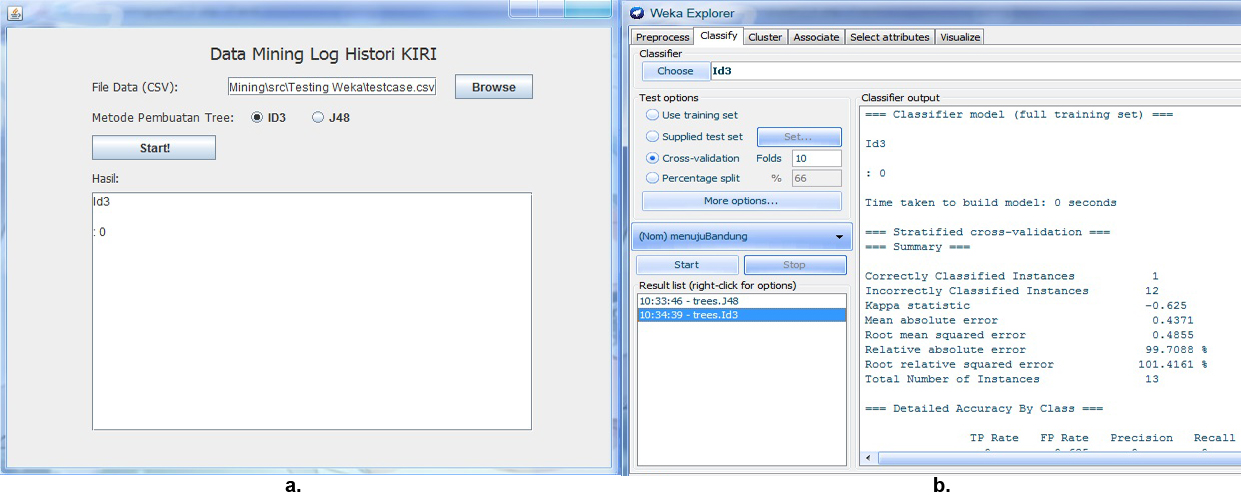
\includegraphics[scale=0.4]{Gambar/pengujian31.jpg}
	\caption[Pengujian Pembuatan \textsl{Decision Tree} ID3]{Pengujian Pembuatan \textsl{Decision Tree} ID3. Gambar a merupakan hasil dari aplikasi \textsl{data mining} sedangkan gambar b merupakan hasil dari weka.} 
	\label{fig:Pengujian31}
	\end{figure}

	\begin{figure}[H]
	\centering
	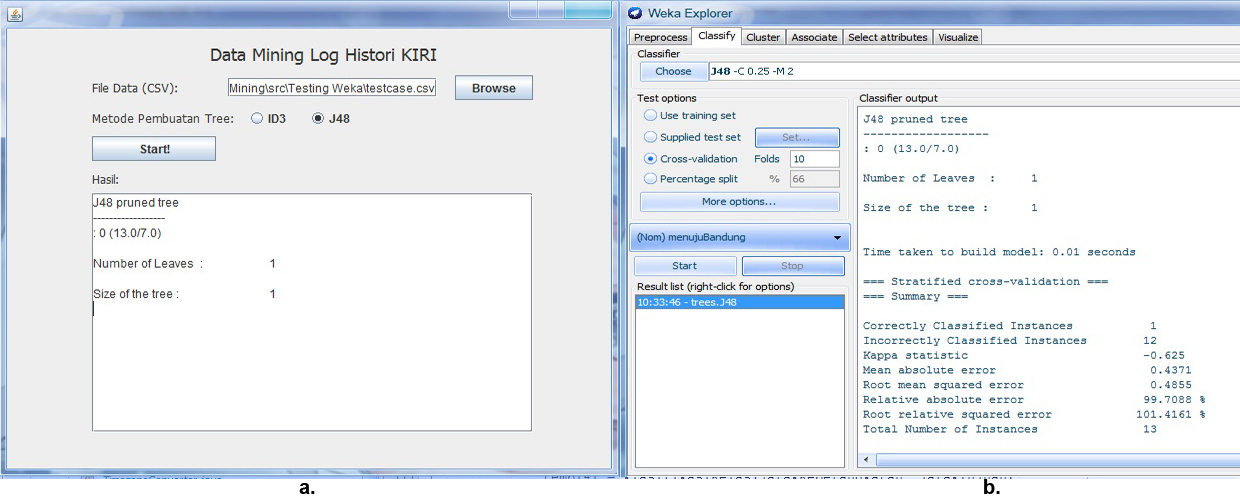
\includegraphics[scale=0.4]{Gambar/pengujian32.jpg}
	\caption[Pengujian Pembuatan \textsl{Decision Tree} J48]{Pengujian Pembuatan \textsl{Decision Tree} J48. Gambar a merupakan hasil dari aplikasi \textsl{data mining} sedangkan gambar b merupakan hasil dari weka.} 
	\label{fig:Pengujian32}
	\end{figure}

	Dari kedua gambar tersebut, dapat disimpulkan bahwa hasil \textsl{decision tree} yang dihasilkan sama dan benar.
	
	\item Pengujian keempat: Mengubah \textsl{decision tree} dalam bentuk String menjadi bahasa DOT, akan dilakukan visualisasi \textsl{decision tree} dengan membuat graph dalam bahasa DOT, dapat dilihat pada gambar \ref{fig:Pengujian4}.
	
	\begin{figure}[H]
	\centering
	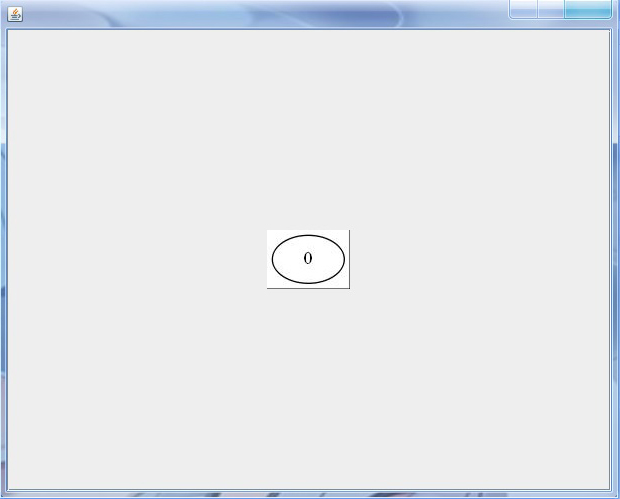
\includegraphics[scale=0.4]{Gambar/pengujian4.jpg}
	\caption[Pengujian Hasil Visualisasi dengan Menggunakan Bahasa DOT]{Pengujian Hasil Visualisasi dengan Menggunakan Bahasa DOT.} 
	\label{fig:Pengujian4}
	\end{figure}
	
	Dari gambar tersebut, dapat disimpulkan bahwa pengubahan \textsl{decision tree} menjadi bahasa DOT telah berhasil.

\end{enumerate}

\subsection{Pengujian Experimental}

Pengujian akan dilakukan pada data 1 bulan dari \textsl{log} histori KIRI pada bulan Febuari dan diperoleh hasil sebagai berikut

\begin{figure}[H]
\centering
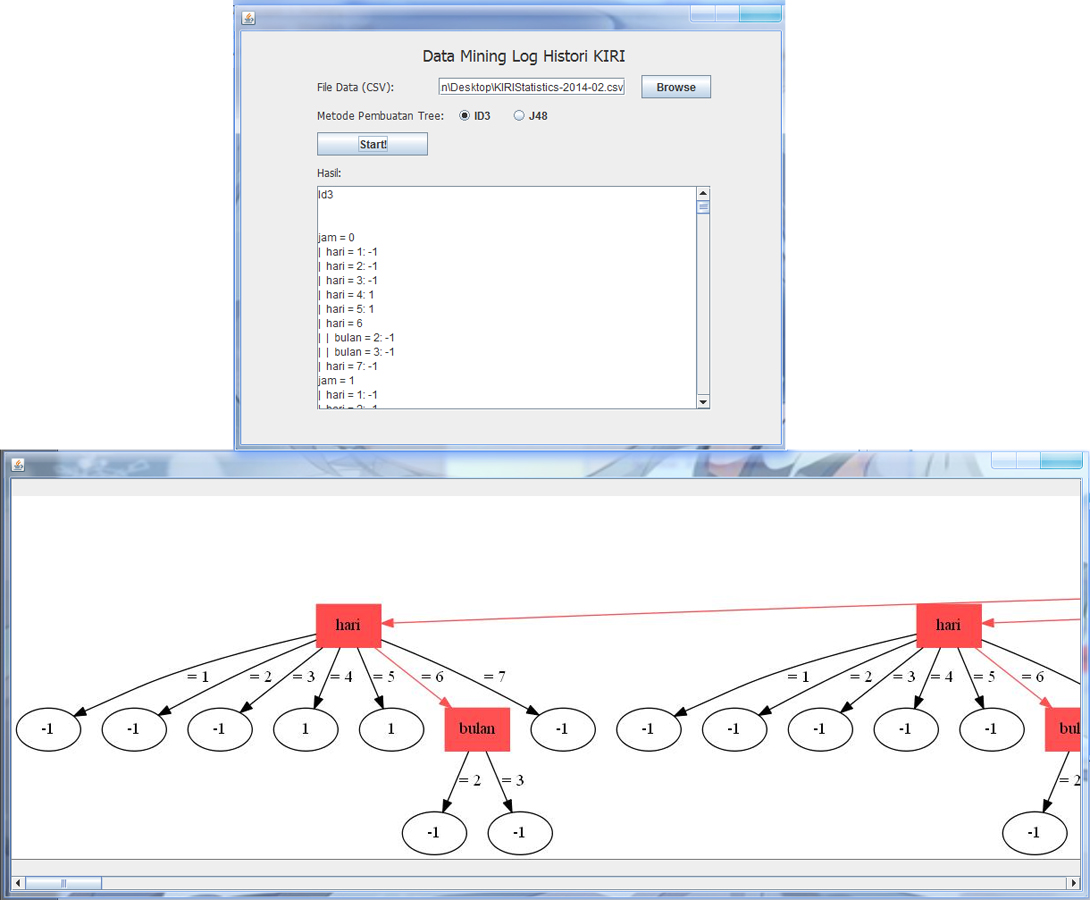
\includegraphics[scale=0.5]{Gambar/percobaan1.jpg}
\caption[Percobaan \textsl{Data Mining} dengan Menggunakan Metode ID3 pada \textsl{Log} Histori KIRI pada Bulan 2 Tahun 2014]{Percobaan \textsl{Data Mining} dengan Menggunakan Metode ID3 pada \textsl{Log} Histori KIRI pada Bulan 2 Tahun 2014.} 
\label{fig:percobaan1}
\end{figure}

\begin{figure}[H]
\centering
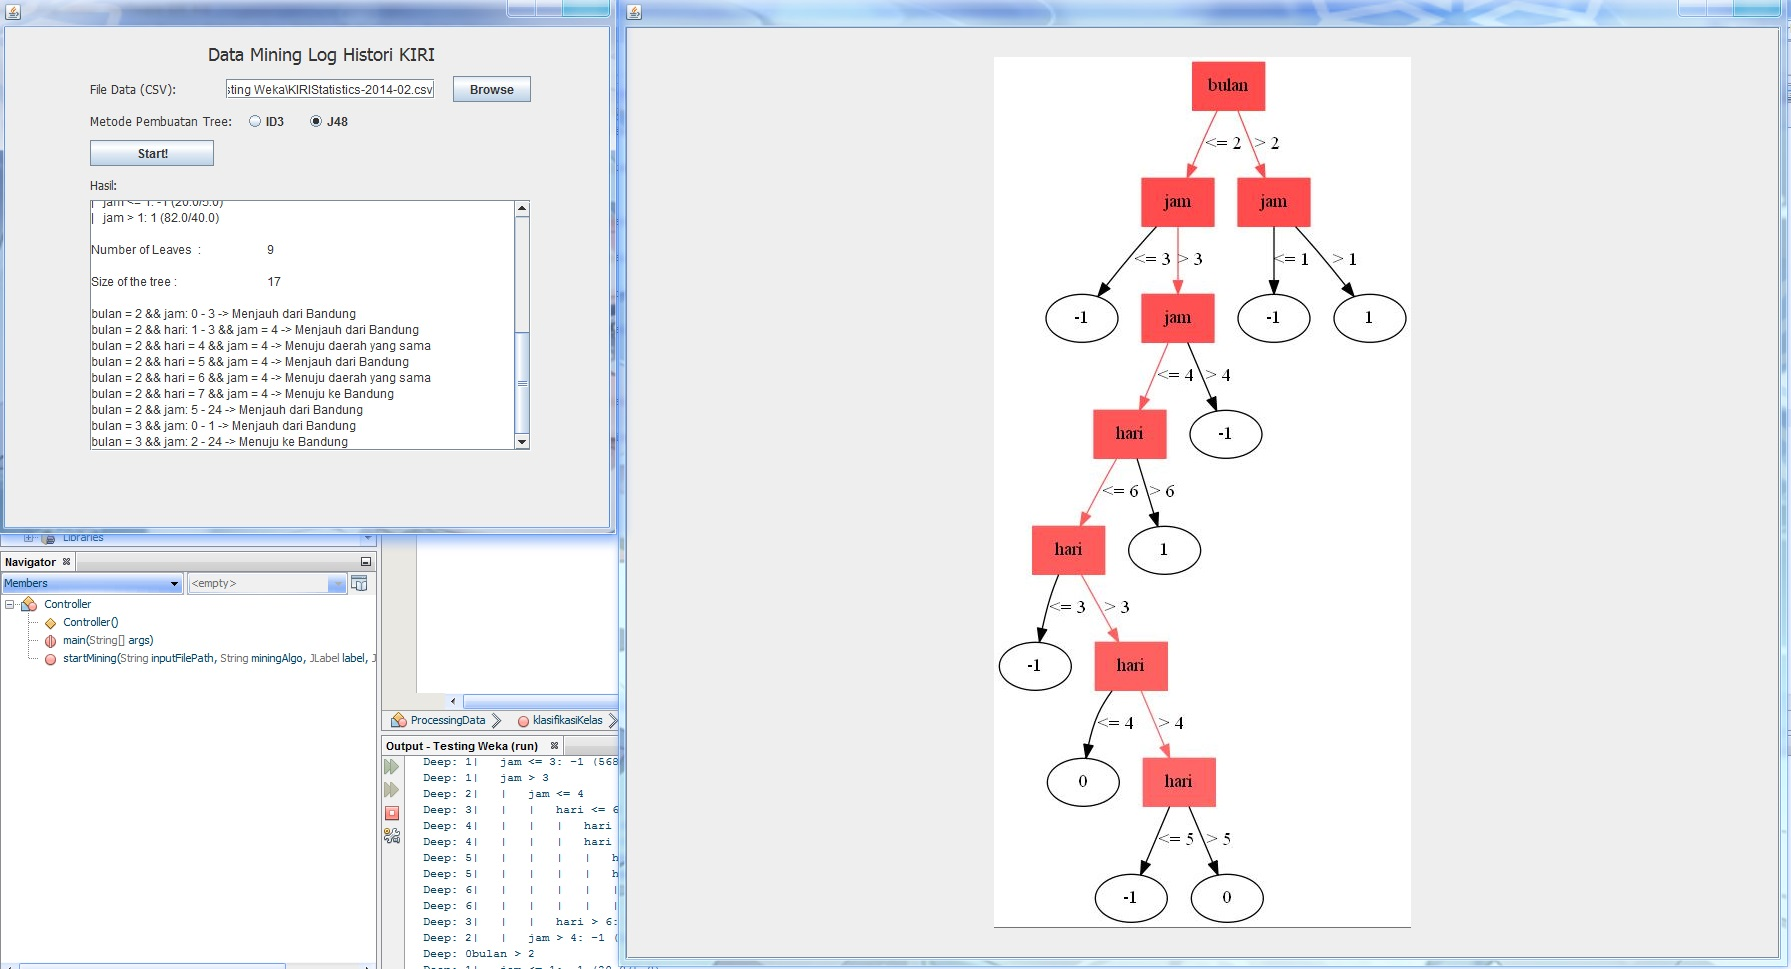
\includegraphics[scale=0.3]{Gambar/percobaan2.jpg}
\caption[Percobaan \textsl{Data Mining} dengan Menggunakan Metode J48 pada \textsl{Log} Histori KIRI pada Bulan 2 Tahun 2014]{Percobaan \textsl{Data Mining} dengan Menggunakan Metode J48 pada \textsl{Log} Histori KIRI pada Bulan 2 Tahun 2014.} 
\label{fig:percobaan2}
\end{figure}

Pada kedua percobaan, terdapat perbedaan bulan, hal ini dikarenakan perubahan waktu dari UTC menuju GMT+7 sehingga terdapat perubahan bulan atau tahun. Karena data pada bulan selanjutnya hanya tujuh jam, maka hasil pada bulan selanjutnya lebih baik tidak dianggap karena data tersebut tidak cukup untuk merepresentasikan waktu satu bulan.

Hasil percobaan pembuatan \textsl{decision tree} pada metode ID3 mengalami overfitting karena menghasilkan klasifikasi pada hampir setiap kemungkinan, dapat disimpulkan hasil \textsl{decision tree} pada percobaan di bulan ini cukup jelek. Namun pada percobaan metode J48, menghasilkan \textsl{decision tree} yang sangat menarik dimana dinyatakan bahwa jam 0-3 dan jam 5-24 user menjauhi Bandung.

Selain itu, dari kedua percobaan ini, diperoleh bahwa cukup sulit untuk membaca hasil \textsl{decision tree} terutama pada \textsl{node} dengan kedalaman lebih dari 4 tingkat. Oleh karena itu, akan ditambahkan fungsi agar \textsl{decision tree} lebih mudah dibaca. Program akan ditambah satu kelas baru yaitu SDForExtractData yang berfungsi untuk menyimpan data dan membuat kesimpulan dari setiap \textsl{leaf} yang dihasilkan. Diagram Kelas untuk kelas SDForExtractData dapat dilihat pada gambar \ref{fig:classDiagramSDForExtractData}. 

\begin{figure}[H]
\centering
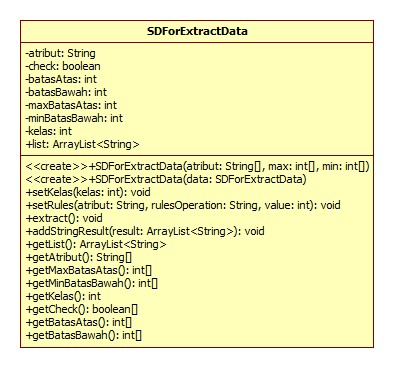
\includegraphics[scale=0.7]{Gambar/SDForExtractData.jpg}
\caption[Diagram Kelas untuk SDForExtractData]{Diagram Kelas untuk SDForExtractData} 
\label{fig:classDiagramSDForExtractData}
\end{figure}

Berikut hasil dari fungsi yang dibuat agar \textsl{decision tree} lebih mudah dibaca, dapat dilihat pada gambar \ref{fig:percobaan3}.

\begin{figure}[H]
\centering
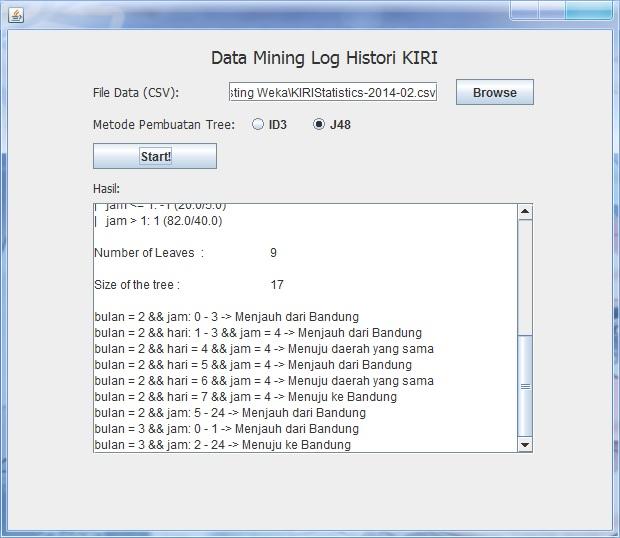
\includegraphics[scale=0.7]{Gambar/percobaan3.jpg}
\caption[Hasil dari SDForExtractData]{Hasil dari SDForExtractData} 
\label{fig:percobaan3}
\end{figure}

Dengan fungsi tersebut, diharapkan user dapat lebih mudah membaca \textsl{decision tree} yang dihasilkan.















}{}
\ifdefstring{\vbabf}{1}{\chapter{Penutup}

\section{Kesimpulan}

Kesimpulan yang dapat diambil dari penelitian \textsl{data mining log} histori KIRI ini adalah 

Salah satu cara untuk memperoleh pola yang menarik dan bermakna, diperlukan pengolahan data dengan cara membuat klasifikasi dari data yang dihasilkan sesuai dengan tujuan yang ingin dicari, pada penelitian ini dilakukan klasifikasi tujuan dari user apakah mereka ingin menuju Bandung atau keluar Bandung atau masih berada di area yang sama sehingga diperoleh pergerakan user KIRI di Bandung. Dari penelitian ini, diperoleh pola yang menarik bahwa user lebih sering menuju luar Bandung pada bulan Febuari 2014.

Cara membuat perangkat lunak untuk melakukan \textsl{data mining} pada \textsl{log} histori KIRI dengan cara 

\section{Saran}

Untuk pengembangan aplikasi \textsl{data mining log} histori KIRI lebih lanjut, dapat dilakukan dengan cara menggunakan klasifikasi yang lebih baik dan detail. Perbedaannya dengan manggunakan klasifikasi yang lebih detail adalah hasil dari \textsl{decision tree} mungkin akan lebih besar namun lebih memiliki makna dan dapat menghasilkan nilai \textsl{confident} yang lebih besar.}{}
\ifdefstring{\vbabg}{1}{\include{Bab/bab7}}{}
\ifdefstring{\vbabh}{1}{\include{Bab/bab8}}{}
\ifdefstring{\vbabi}{1}{\include{Bab/bab9}}{}

\bibliographystyle{ieeetr}
\bibliography{pustaka}

\appendix
\apptoc

\tampillmp{\vlmp}
\begin{landscape}
\ifdefstring{\vlmpa}{1}{\chapter{100 data pertama dari \textsl{log} histori KIRI}
%\label{app:A}

\begin{table}[h]
\begin{tabular}{|l|l|l|l|l|}
\hline
\textbf{LogId} & \textbf{APIKey}  & \textbf{Timestamp (UTC)} & \textbf{Action} & \textbf{AddionalData}                                                                                                                                                                                                 \\ \hline
113909         & E5D9904F0A8B4F99 & 2/1/2014 0:07            & PAGELOAD        & /5.10.83.30/                                                                                                                                                                                                          \\ \hline
113910         & E5D9904F0A8B4F99 & 2/1/2014/ 0:07           & PAGELOAD        & /5.5.83.49/                                                                                                                                                                                                           \\ \hline
113911         & E5D9904F0A8B4F99 & 2/1/2014/ 0:09           & PAGELOAD        & /5.10.83.30/                                                                                                                                                                                                          \\ \hline
113912         & E5D9904F0A8B4F99 & 2/1/2014 0:10            & PAGELOAD        & /5.10.83.88/                                                                                                                                                                                                          \\ \hline
113913         & E5D9904F0A8B4F99 & 2/1/2014 0:10            & PAGELOAD        & /5.10.83.58/                                                                                                                                                                                                          \\ \hline
113914         & A44EB361A179A49E & 2/1/2014 0:11            & SEARCHPLACE     & taman+fot/10                                                                                                                                                                                                          \\ \hline
113915         & A44EB361A179A49E & 2/1/2014 0:11            & FINDROUTE       & -6.8972513,107.6385574/-6.91358,107.62718/1                                                                                                                                                                           \\ \hline
113916         & E5D9904F0A8B4F99 & 2/1/2014 0:12            & PAGELOAD        & /5.10.83.24/                                                                                                                                                                                                          \\ \hline
113917         & 81CC9E4AD224357E & 2/1/2014 0:13            & WIDGETLOAD      & /192.95.25.92/                                                                                                                                                                                                        \\ \hline
11318          & A44EB361A179A49E & 2/1/2014 0:13            & SEARCHPLACE     & taman+f/10                                                                                                                                                                                                            \\ \hline
113919         & A44EB361A179A49E & 2/1/2014 0:13            & FINDROUTE       & -6.8972513,107.6385574/-6.91358,107.62718/1                                                                                                                                                                           \\ \hline
113920         & D0AB08D956A351E4 & 2/1/2014 0:15            & FINDROUTE       & -6.90598,107.59714/-6.90855,107.61082/1                                                                                                                                                                               \\ \hline
113921         & D0AB08D956A351E4 & 2/1/2014 0:16            & SEARCHPLACE     & istanta/0                                                                                                                                                                                                             \\ \hline
113922         & D0AB08D956A351E4 & 2.1.2014 0:16            & SEARCHPLACE     & istaba/0                                                                                                                                                                                                              \\ \hline
113923         & D0AB08D956A351E4 & 2/1/2014 0:16            & FINDROUTE       & -6.90598,107.59714/-6.90855,107.61082/1                                                                                                                                                                               \\ \hline
113924         & D0AB08D956A351E4 & 2/1/2014 0:17            & FINDROUTE       & -6.90598,107.59714/-6.90855,107.61082/1                                                                                                                                                                               \\ \hline
113925         & A44EB361A179A49E & 2/1/2014 0:18            & SEARCHPLACE     & kantor+po/10                                                                                                                                                                                                          \\ \hline
113926         & A44EB361A179A49E & 2/1/2014 0:18            & SEARCHPLACE     & kantor+pos/10                                                                                                                                                                                                         \\ \hline
113927         & A44EB361A179A49E & 2/1/2014 0:18            & SEARCHPLACE     & kantor+pos+ci/10                                                                                                                                                                                                      \\ \hline
113928         & A44EB361A179A49E & 2/1/2014 0:18            & SEARCHPLACE     & kantor+pos+cimahi/10                                                                                                                                                                                                  \\ \hline
113929         & A44EB361A179A49E & 2/1/2014 0:18            & FINDROUTE       & -6.7185828,107.0150728/-6.918881548242062,107.60667476803064/1                                                                                                                                                        \\ \hline
113930         & A44EB361A179A49E & 2/1/2014 0:18            & FINDROUTE       & -6.9015366,107.5414474/-6.88574,107.53816/1                                                                                                                                                                           \\ \hline
113931         & E5D9904F0A8B4F99 & 2/1/2014 0:22            & PAGELOAD        & /5.10.83.49/                                                                                                                                                                                                          \\ \hline
113932         & E5D9904F0A8B4F99 & 2/1/2014 0:22            & PAGELOAD        & /180.253.140.219/                                                                                                                                                                                                     \\ \hline
113933         & E5D9904F0A8B4F99 & 2/1/2014 0:24            & PAGELOAD        & /180.253.140.219/                                                                                                                                                                                                     \\ \hline
113934         & E5D9904F0A8B4F99 & 2/1/2014 0:25            & PAGELOAD        & /180.253.140.219/                                                                                                                                                                                                     \\ \hline
113935         & E5D9904F0A8B4F99 & 2/1/2014 0:25            & FINDROUTE       & -6.90608,107.61530/-6.89140,107.61060/2                                                                                                                                                                               \\ \hline
113936         & E5D9904F0A8B4F99 & 2/1/2014 0:26            & PAGELOAD        & /118.137.96.28/                                                                                                                                                                                                       \\ \hline
113937         & E5D9904F0A8B4F99 & 2/1/2014 0:26            & FINDROUTE       & -6.89459,107.58818/-6.89876,107.60886/2                                                                                                                                                                               \\ \hline
113938         & E5D9904F0A8B4F99 & 2/1/2014 0:27            & FINDROUTE       & -6.90608,107.61530/-6.89140,107.61060/2                                                                                                                                                                               \\ \hline
113939         & E5D9904F0A8B4F99 & 2/1/2014 0:28            & FINDROUTE       & -6.89977,107.62706/-6.89140,107.61060/2                                                                                                                                                                               \\ \hline
113940         & E5D9904F0A8B4F99 & 2/1/2014 0:28            & FINDROUTE       & -6.89459,107.58818/-6.86031,107.61287/2                                                                                                                                                                               \\ \hline
113941         & D0AB08D956A351E4 & 2/1/2014 0:28            & FINDROUTE       & -6.90598,107.59714/-6.90855,107.61082/1                                                                                                                                                                               \\ \hline
113942         & A44EB361A179A49E & 2/1/2014 0:29            & FINDROUTE       & -6.9172304,107.6042556/-6.92663,107.63644/1                                                                                                                                                                           \\ \hline
113943         & A44EB361A179A49E & 2/1/2014 0:29            & FINDROUTE       & -6.9172448,107.6042255/-6.92663,107.63644/1                                                                                                                                                                           \\ \hline
113944         & D0AB08D956A351E4 & 2/1/2014 0:30            & FINDROUTE       & -6.90598,107.59714/-6.90855,107.61082/1                                                                                                                                                                               \\ \hline
113945         & D0AB08D956A351E4 & 2/1/2014 0:32            & FINDROUTE       & -6.90598,107.59714/-6.90855,107.61082/1                                                                                                                                                                               \\ \hline
113946         & D0AB08D956A351E4 & 2/1/2014 0:33            & FINDROUTE       & -6.90598,107.59714/-6.90855,107.61082/1                                                                                                                                                                               \\ \hline
113947         & A44EB361A179A49E & 2/1/2014 0:35            & SEARCHPLACE     & jalan+asia+af/8                                                                                                                                                                                                       \\ \hline
113948         & A44EB361A179A49E & 2/1/2014 0:35            & FINDROUTE       & -6.9172448,107.6042255/-6.92163,107.61046/1                                                                                                                                                                           \\ \hline
113949         & A44EB361A179A49E & 2/1/2014 0:35            & SEARCHPLACE     & taman+fotog/10                                                                                                                                                                                                        \\ \hline
113950         & A44EB361A179A49E & 2/1/2014 0:36            & FINDROUTE       & -6.917321,107.6043132/-6.921568846707516,107.61015225201845/1                                                                                                                                                         \\ \hline
113951         & E5D9904F0A8B4F99 & 2/1/2014 0:38            & PAGELOAD        & /5.10.83.68/                                                                                                                                                                                                          \\ \hline
113952         & E5D9904F0A8B4F99 & 2/1/2014 0:38            & PAGELOAD        & /5.10.83.28/                                                                                                                                                                                                          \\ \hline
113953         & E5D9904F0A8B4F99 & 2/1/2014 0:40            & PAGELOAD        & /206.53.152.81/m                                                                                                                                                                                                      \\ \hline
113954         & E5D9904F0A8B4F99 & 2/1/2014 0:40            & FINDROUTE       & -6.90598,107.59714/-6.91728,107.60417/1                                                                                                                                                                               \\ \hline
113955         & E5D9904F0A8B4F99 & 2/1/2014 0:41            & PAGELOAD        & /5.10.83.30/                                                                                                                                                                                                          \\ \hline
113956         & E5D9904F0A8B4F99 & 2/1/2014 0:40            & PAGELOAD        & /5.10.83.28/                                                                                                                                                                                                          \\ \hline
113957         & E5D9904F0A8B4F99 & 2/1/2014 0:55            & PAGELOAD        & /5.10.83.99/                                                                                                                                                                                                          \\ \hline
113958         & D0AB08D956A351E4 & 2/1/2014 1:00            & SEARCHPLACE     & babd/1                                                                                                                                                                                                                \\ \hline
113959         & D0AB08D956A351E4 & 2/1/2014 1:00            & SEARCHPLACE     & babdu/1                                                                                                                                                                                                               \\ \hline
113960         & D0AB08D956A351E4 & 2/1/2014 1:00            & FINDROUTE       & -6.90598,107.59714/-6.90855,107.61082/1                                                                                                                                                                               \\ \hline
113961         & D0AB08D956A351E4 & 2/1/2014 1:09            & FINDROUTE       & -6.38355,106.919975/-6.85029,107.58496/1                                                                                                                                                                              \\ \hline
113962         & D0AB08D956A351E4 & 2/1/2014 1:10            & FINDROUTE       & -6.90598,107.59714/-6.85029,107.58496/1                                                                                                                                                                               \\ \hline
113963         & D0AB08D956A351E4 & 2/1/2014 1:10            & FINDROUTE       & -6.90598,107.59714/-6.90855,107.61082/1                                                                                                                                                                               \\ \hline
113964         & E5D9904F0A8B4F99 & 2/1/2014 1:10            & PAGELOAD        & /5.10.83.49/                                                                                                                                                                                                          \\ \hline
113965         & D0AB08D956A351E4 & 2/1/2014 1:12            & SEARCHPLACE     & tea/10                                                                                                                                                                                                                \\ \hline
113966         & A44EB361A179A49E & 2/1/2014 1:15            & SEARCHPLACE     & taman+pustaka/10                                                                                                                                                                                                      \\ \hline
113967         & A44EB361A179A49E & 2/1/2014 1:15            & SEARCHPLACE     & taman+pustaka+besarn/8                                                                                                                                                                                                \\ \hline
113968         & A44EB361A179A49E & 2/1/2014 1:15            & FINDROUTE       & -6.9135911,107.6272095/-6.90179,107.62301/1                                                                                                                                                                           \\ \hline
113969         & E5D9904F0A8B4F99 & 2/1/2014 1:16            & PAGELOAD        & /36.72.98.13/                                                                                                                                                                                                         \\ \hline
113970         & E5D9904F0A8B4F99 & 2/1/2014 1:17            & PAGELOAD        & /120.173.21.110/m                                                                                                                                                                                                     \\ \hline
113971         & E5D9904F0A8B4F99 & 2/1/2014 1:17            & SEARCHPLACE     & jalan+abdrrahman+saleh/10                                                                                                                                                                                             \\ \hline
113972         & E5D9904F0A8B4F99 & 2/1/2014 1:17            & FINDROUTE       & -6.90872,107.62253/-6.90774,107.60908/1                                                                                                                                                                               \\ \hline
113973         & A44EB361A179A49E & 2/1/2014 1:19            & FINDROUTE       & -6.9158359,107.6101751/-6.90691,107.62259/1                                                                                                                                                                           \\ \hline
113974         & E5D9904F0A8B4F99 & 2/1/2014 1:19            & FINDROUTE       & -6.91335,107.64827/-6.86198,107.59193/1                                                                                                                                                                               \\ \hline
113975         & E5D9904F0A8B4F99 & 2/1/2014 1:25            & PAGELOAD        & /114.79.13.124/                                                                                                                                                                                                       \\ \hline
113976         & E5D9904F0A8B4F99 & 2/1/2014 1:25            & PAGELOAD        & /5.10.83.24/                                                                                                                                                                                                          \\ \hline
113977         & E5D9904F0A8B4F99 & 2/1/2014 1:25            & FINDROUTE       & -6.91485,107.59123/-6.91593,107.65588/1                                                                                                                                                                               \\ \hline
113978         & E5D9904F0A8B4F99 & 2/1/2014 1:26            & PAGELOAD        & /5.10.83.82/                                                                                                                                                                                                          \\ \hline
113979         & E5D9904F0A8B4F99 & 2/1/2014 1:28            & FINDROUTE       & -6.91593,107.65588/-6.91485,107.59123/1                                                                                                                                                                               \\ \hline
113980         & A44EB361A179A49E & 2/1/2014 1:29            & FINDROUTE       & -6.9250709,107.6204635/-6.91728,107.60417/1                                                                                                                                                                           \\ \hline
113981         & A44EB361A179A49E & 2/1/2014 1:35            & FINDROUTE       & -6.9252132,107.6200288/-6.91728,107.60417/1                                                                                                                                                                           \\ \hline
113982         & A44EB361A179A49E & 2/1/2014 1:36            & FINDROUTE       & -6.922427886995373,107.61768691241741/-6.91728,107.60417/1                                                                                                                                                            \\ \hline
113983         & E5D9904F0A8B4F99 & 2/1/2014 1:36            & FINDROUTE       & -6.91431,107.63921/-6.94024,107.71550/1                                                                                                                                                                               \\ \hline
113984         & E5D9904F0A8B4F99 & 2/1/2014 1:37            & PAGELOAD        & /5.10.83.98/                                                                                                                                                                                                          \\ \hline
113985         & A44EB361A179A49E & 2/1/2014 1:37            & FINDROUTE       & -6.921635413232821,107.61909071356058/-6.91728,107.60417/1                                                                                                                                                            \\ \hline
113986         & E5D9904F0A8B4F99 & 2/1/2014 1:38            & FINDROUTE       & -6.88936,107.57533/-6.92600,107.63628/1                                                                                                                                                                               \\ \hline
113987         & E5D9904F0A8B4F99 & 2/1/2014 1:39            & PAGELOAD        & http://www.kiri.travel/m/r/?qs=trans+studio+mall\&qf=sukamekar\&ls=-6.92600\%2C107.63628\&lf=-6.88936\%2C107.57533\&s=Trans+Studio+Mall+\%28TSM\%29+-+Jalan+Gatot+Subroto+No.+289\&f=Sukamekar\&l=en/180.214.232.82/m \\ \hline
113988         & E5D9904F0A8B4F99 & 2/1/2014 1:39            & FINDROUTE       & -6.92600,107.63628/-6.88936,107.57533/1                                                                                                                                                                               \\ \hline
113989         & A44EB361A179A49E & 2/1/2014 1:41            & SEARCHPLACE     & terminal+ta/10                                                                                                                                                                                                        \\ \hline
113990         & A44EB361A179A49E & 2/1/2014 1:41            & FINDROUTE       & -6.9158359,107.6101751/-6.90658,107.61623/1                                                                                                                                                                           \\ \hline
113991         & A44EB361A179A49E & 2/1/2014 1:42            & FINDROUTE       & -6.9158359,107.6101751/-6.90658,107.61623/1                                                                                                                                                                           \\ \hline
113992         & D0AB08D956A351E4 & 2/1/2014 1:50            & FINDROUTE       & -6.38355,106.919975/-7.08933734335005,107.562576737255/1                                                                                                                                                              \\ \hline
113993         & A44EB361A179A49E & 2/1/2014 1:51            & SEARCHPLACE     & taman+ci/10                                                                                                                                                                                                           \\ \hline
113994         & A44EB361A179A49E & 2/1/2014 1:51            & SEARCHPLACE     & taman+cilaki/10                                                                                                                                                                                                       \\ \hline
113995         & E5D9904F0A8B4F99 & 2/1/2014 1:52            & PAGELOAD        & /206.53.152.33/m                                                                                                                                                                                                      \\ \hline
113996         & E5D9904F0A8B4F99 & 2/1/2014 1:52            & FINDROUTE       & -6.90598,107.59714/-6.91728,107.60417/1                                                                                                                                                                               \\ \hline
113997         & A44EB361A179A49E & 2/1/2014 1:54            & FINDROUTE       & -6.901306,107.6214169/-6.90336,107.62235/1                                                                                                                                                                            \\ \hline
113998         & A44EB361A179A49E & 2/1/2014 1:54            & FINDROUTE       & -6.901306,107.6214169/-6.90336,107.62235/1                                                                                                                                                                            \\ \hline
113999         & E5D9904F0A8B4F99 & 2/1/2014                 & PAGELOAD        & /5.10.83.27/                                                                                                                                                                                                          \\ \hline
114000         & 308201BB30820124 & 2/1/2014 1:15            & SEARCHPLACE     & riau+jucntion/10                                                                                                                                                                                                      \\ \hline
114001         & 308201BB30820124 & 2/1/2014 1:56            & FINDROUTE       & -6.90687,107.61239/-6.89032,107.57961/2                                                                                                                                                                               \\ \hline
114002         & E5D9904F0A8B4F99 & 2/1/2014 1:57            & PAGELOAD        & /118.99.112.66/                                                                                                                                                                                                       \\ \hline
114003         & 308201BB30820124 & 2/1/2014 1:57            & FINDROUTE       & -6.90687,107.61239/-6.90159,107.60442/1                                                                                                                                                                               \\ \hline
114004         & 308201BB30820124 & 2/1/2014 1:57            & FINDROUTE       & -6.90687,107.61239/-6.89032,107.57961/2                                                                                                                                                                               \\ \hline
114005         & E5D9904F0A8B4F99 & 2/1/2014 1:58            & FINDROUTE       & -6.88211,107.60378/-6.90774,107.60908/1                                                                                                                                                                               \\ \hline
114006         & A44EB361A179A49E & 2/1/2014 1:59            & FINDROUTE       & -6.9212516,107.6196466/-6.91728,107.60417/1                                                                                                                                                                           \\ \hline
114007         & 308201BB30820124 & 2/1/2014 1:59            & FINDROUTE       & -6.90687,107.61239/-6.91486,107.60824/1                                                                                                                                                                               \\ \hline
114008         & 687C44EB2424285D & 2/1/2014 1:59            & WIDGETLOAD      & http://www.cendekialeadershipschool.sch.id//112.215.36.143/                                                                                                                                                           \\ \hline
114009         & E5D9904F0A8B4F99 & 2/1/2014 2:00            & FINDROUTE       & -6.88166,107.61561/-6.90774,107.60908/1                                                                                                                                                                               \\ \hline
\end{tabular}
\end{table}}{}
\end{landscape}
\ifdefstring{\vlmpb}{1}{\chapter{The Source Code}
\label{app:B}

%selalu gunakan single spacing untuk source code !!!!!
\singlespacing 
% language: bahasa dari kode program
% terdapat beberapa pilihan : Java, C, C++, PHP, Matlab, R, dll
%
% basicstyle : ukuran font untuk kode program
% terdapat beberapa pilihan : tiny, scriptsize, footnotesize, dll
%
% caption : nama yang akan ditampilkan di dokumen akhir, lihat contoh
\begin{lstlisting}[language=Java,basicstyle=\tiny,caption=MyFurSet.java]

import java.util.ArrayList;
import java.util.Collections;
import java.util.HashSet;

/**
 *
 * @author Lionov
 */

//class for set of vertices close to furthest edge
public class MyFurSet {
    protected int id;                                  //id of the set
    protected MyEdge FurthestEdge;                     //the furthest edge
    protected HashSet<MyVertex> set;                   //set of vertices close to furthest edge
    protected ArrayList<ArrayList<Integer>> ordered;   //list of all vertices in the set for each trajectory
    protected ArrayList<Integer> closeID;              //store the ID of all vertices
    protected ArrayList<Double> closeDist;             //store the distance of all vertices
    protected int totaltrj;                            //total trajectories in the set

    /**
     * Constructor
     * @param id : id of the set
     * @param totaltrj : total number of trajectories in the set
     * @param FurthestEdge : the furthest edge
     */
    public MyFurSet(int id,int totaltrj,MyEdge FurthestEdge) {
        this.id = id;
        this.totaltrj = totaltrj;
        this.FurthestEdge = FurthestEdge;
        set = new HashSet<MyVertex>();
        ordered = new ArrayList<ArrayList<Integer>>();
        for (int i=0;i<totaltrj;i++) ordered.add(new ArrayList<Integer>());
        closeID = new ArrayList<Integer>(totaltrj);
        closeDist = new ArrayList<Double>(totaltrj);
        for (int i = 0;i <totaltrj;i++) {
            closeID.add(-1);
            closeDist.add(Double.MAX_VALUE);
        }
    }

    /**
     * set a vertex into the set
     * @param v : vertex to be added to the set
     */
    public void add(MyVertex v) {
        set.add(v);
    }

    /**
     * check whether vertex v is a member of the set
     * @param v : vertex to be checked
     * @return true if v is a member of the set, false otherwise
     */
    public boolean contains(MyVertex v) {
        return this.set.contains(v);
    }
}
\end{lstlisting}}{}
%\ifdefstring{\vlmpc}{1}{\chapter{The Source Code}
\label{app:C}

%selalu gunakan single spacing untuk source code !!!!!
\singlespacing 
% language: bahasa dari kode program
% terdapat beberapa pilihan : Java, C, C++, PHP, Matlab, R, dll
%
% basicstyle : ukuran font untuk kode program
% terdapat beberapa pilihan : tiny, scriptsize, footnotesize, dll
%
% caption : nama yang akan ditampilkan di dokumen akhir, lihat contoh
\begin{lstlisting}[language=Java,basicstyle=\tiny,caption=MyFurSet.java]

import java.util.ArrayList;
import java.util.Collections;
import java.util.HashSet;

/**
 *
 * @author Lionov
 */

//class for set of vertices close to furthest edge
public class MyFurSet {
    protected int id;                                  //id of the set
    protected MyEdge FurthestEdge;                     //the furthest edge
    protected HashSet<MyVertex> set;                   //set of vertices close to furthest edge
    protected ArrayList<ArrayList<Integer>> ordered;   //list of all vertices in the set for each trajectory
    protected ArrayList<Integer> closeID;              //store the ID of all vertices
    protected ArrayList<Double> closeDist;             //store the distance of all vertices
    protected int totaltrj;                            //total trajectories in the set

    /**
     * Constructor
     * @param id : id of the set
     * @param totaltrj : total number of trajectories in the set
     * @param FurthestEdge : the furthest edge
     */
    public MyFurSet(int id,int totaltrj,MyEdge FurthestEdge) {
        this.id = id;
        this.totaltrj = totaltrj;
        this.FurthestEdge = FurthestEdge;
        set = new HashSet<MyVertex>();
        ordered = new ArrayList<ArrayList<Integer>>();
        for (int i=0;i<totaltrj;i++) ordered.add(new ArrayList<Integer>());
        closeID = new ArrayList<Integer>(totaltrj);
        closeDist = new ArrayList<Double>(totaltrj);
        for (int i = 0;i <totaltrj;i++) {
            closeID.add(-1);
            closeDist.add(Double.MAX_VALUE);
        }
    }

    /**
     * set a vertex into the set
     * @param v : vertex to be added to the set
     */
    public void add(MyVertex v) {
        set.add(v);
    }

    /**
     * check whether vertex v is a member of the set
     * @param v : vertex to be checked
     * @return true if v is a member of the set, false otherwise
     */
    public boolean contains(MyVertex v) {
        return this.set.contains(v);
    }

    /**
     *  create a column for table Gamma, sorted for each row
     */
    public void createColumn() {
        for (MyVertex v : set) {
            for (Integer key : v.vertexnum.keySet()) {
                for (Integer values : v.vertexnum.get(key)) {
                    ordered.get(key).add(values);
                }
            }
        }
        for (ArrayList<Integer> al : ordered) Collections.sort(al);
    }


}
\end{lstlisting}}{}
%\ifdefstring{\vlmpd}{1}{\include{Lampiran/lampD}}{}
%\ifdefstring{\vlmpe}{1}{\include{Lampiran/lampE}}{}
%\ifdefstring{\vlmpf}{1}{\include{Lampiran/lampF}}{}
%\ifdefstring{\vlmpg}{1}{\include{Lampiran/lampG}}{}
%\ifdefstring{\vlmph}{1}{\include{Lampiran/lampH}}{}
%\ifdefstring{\vlmpi}{1}{\include{Lampiran/lampI}}{}

\end{document}
